%%%%%%%%%%%%%%%%%%%%%%%%%%%%%%%%%%%%%%%%%%%%%%%%%%%%%%%%%%%%%%%%%%%%%%%%%%
%% This template was created by Nathan Rountree 9/2/98
%% Updates have since been made by others in the department.
%%
%%%%%%%%%%%%%%%%%%%%%%%%%%%%%%%%%%%%%%%%%%%%%%%%%%%%%%%%%%%%%%%%%%%%%%%%%%%

%%
%% In the style of a technical report, in 12pt and one sided.
%% Start chapters on right hand side pages only.
%%
\documentclass[12pt]{report}    
%%\documentclass[12pt,twoside,openright]{report} %% Use this for twosided.

%%
%% Load packages.
%%
\usepackage[phd]{otagothesis}     %% Use Otago page layout

\usepackage[round,sectionbib,comma,sort&compress]{natbib}
\usepackage{chapterbib}%% Use Natural Sciences bibliography

\usepackage[T1]{fontenc} %% assist clipboard copy from PDF; allow < | > etc.
\usepackage[utf8x]{inputenc}  %% allow UTF-8 conent in source files
\usepackage{mathpazo}
%%\usepackage[sfdefault]{cabin} %% Use nicer fonts
\usepackage{times}              %% Times PostScript font. Don't use
				  %% if thesis contains lots of math.
\usepackage{flexisym} % for weird symbols
\usepackage{textgreek}
\usepackage{numprint}
\usepackage[rightcaption]{sidecap}
\usepackage{float}
\usepackage{booktabs}
\usepackage{longtable}
\usepackage{graphicx}             %% jpg, gif, tiff, and pdf graphics
\usepackage{moreverb}             %% Verbatim Code Listings
\usepackage{wrapfig}
\usepackage{caption, subcaption}
\captionsetup{font=footnotesize, labelfont=bf}
\usepackage{floatrow}
\usepackage[final]{pdfpages}
%%
%% Set title, author and date.
%%
\title{Pathogen Genomics}
\author{Bethany R. Jose}
\date{6\textsuperscript{th} of December, 2019}

%%
%% The library want to know all sorts of personal stuff!
%% Can be left out if you don't use the \frontstuff command
%%
\fullname{Bethany Rebecca Jose}
\department{Department of Biochemistry}
\dob{22 December 1990} %% date-of-birth
\address{710 Cumberland Street, North Dunedin, Dunedin, NZ}

%%
%% Uncomment to just print up a few chapters.
%%
%%\includeonly{literature,conclusion}


\begin{document}

%%
%% Put in titlepage and contents, etc...
%%
%\frontstuff
\linespread{1.3}
\normalsize

%%
%% Include each chapter as a separate file.
%% These lines assume there are files called intro.tex, literature.tex etc.
%%
\setlength\parindent{0pt}
\setlength{\parskip}{6pt}

\chapter{An introduction to RNA bioinformatics and pathogen genomics}
\label{chap:intro}
\section{Preface}
Bacteria are the most diverse and abundant type of organism on the planet \citep{Hug2016-nr}. Among the multitude of possible evolutionary niches, only a small subset of bacteria occupy pathogenic roles \citep{noauthor_2011-sb,Balloux2017}. Bacterial pathogens exhibit a remarkable range of adaptions to survive stresses encountered both in the environment and within the host. These include the acquisition of new genes \textit{via} horizontal transfer \citep{Kado2009-eh,Groisman1996-fv}, as well as changes in both gene function \citep{Moxon1994-oe} and gene expression \citep{Thomas2014-ln}.
Despite having far fewer genes than eukaryotes, sophisticated regulatory networks allow bacteria to sense and respond to their environment \citep{Dorman2018-dv}. The regulatory function and evolution of many non-coding RNAs (ncRNAs) have been identified as major contributors to the virulence and survival of many bacterial pathogens \citep{Gottesman2005-cp,Gripenland2010-rm}. Of particular interest are the small non-coding RNAs (sRNAs) that participate in regulatory networks \textit{via} interactions with mRNA and proteins \citep{Gottesman2011-vx}.\par

This thesis will primarily focus on the technicalities of identifying and studying non-coding RNA sequences in bacterial pathogens. Specifically, within the genus \textit{Salmonella} and other pathogens of the Enterobacteriaceae that infect animals and plants, and the kiwifruit pathogen \textit{Pseudomonas syringae} pv. \textit{actinidiae}, also known as \textit{Psa}.\par

\section{A brief introduction to genomics}
Pathogen genomics is largely the analysis of biological sequences to identify features which directly or indirectly influence the virulence and fitness of pathogens. This may involve the identification of antibiotic resistance genes, virulence factors such as toxins, or track the evolution and horizontal gene transfer of such elements. The large scale study of such information has been facilitated by the introduction of next-generation sequencing (NGS) technologies, which are both increasingly affordable and capable of producing vast quantities of sequence data \citep{Goodwin2016-on}. As a result, the number of bacterial genome sequences available for comparison has increased exponentially (Figure \ref{fig:path_graph}).
\begin{figure}[H]
  \includegraphics[scale=0.65]{intro/path_graph.png}
  \centering
  \caption[Total prokaryotic genome submissions to NCBI over time]{Total prokaryotic genome submissions to NCBI over time, showing the exponential growth in prokaryotic genome submissions. Data taken from the NCBI prokaryote genome assembly summary  (ftp://ftp.ncbi.nlm.nih.gov/genomes/GENOME_REPORTS/prokaryotes.txt, date range 1995-2018). Relative proportions of pathogenic species and strains identified as pathogenic by \cite{Ecker2005} are shown as coloured stacks grouped by genera, showing that the majority of prokaryotic genomes in NCBI are from pathogenic species. The top 6 genera are ordered by proportion from smallest to largest (\textit{Pseudomonas}, \textit{Klebsiella}, \textit{Mycobacterium}, \textit{Staphylococcus}, \textit{Escherichia} and \textit{Streptococcus}), with "Other" representing the combined sum of remaining pathogen genomes.}
  \label{fig:path_graph}
\end{figure}
Despite representing a tiny fraction of microbial diversity \citep{Balloux2017}, prokaryotic pathogens are over-represented within genome databases (Figure \ref{fig:path_graph}). Genera such as \textit{Streptococcus}, \textit{Escherichia}, and \textit{Salmonella} that contain multiple pathogenic species have been densely sampled, facilitating increasingly detailed and granular genomic studies of pathogenic bacteria.\par

Genomics, the study of genome sequences, is intertwined with the field of bioinformatics, which is tasked with both managing and interpreting these increasingly large amounts of sequence data. Early bioinformatics tools for biological sequence analysis were designed to assemble \citep{Dayhoff:1962:CCP:1461518.1461546,Staden1979} and compare \citep{NEEDLEMAN1970443,Smith_Waterman_1981,Thompson_Higgins_Gibson_1994,Felsenstein_1981} amino acid and nucleotide sequences, which may be simply represented as character strings in a computing context \citep{Gauthier2018-bk}.\par
Much of modern bioinformatics remains focused on these same problems; studying both the information content within, and comparisons between biological sequences. Detailed introductions to these methods can be found in numerous textbooks covering bioinformatics methods and algorithms, e.g \cite{Eddy_BSA_1998,Mount_2004} and \cite{Waterman_1995}.

\subsection{Next Generation Sequencing technologies}
The introduction of NGS technologies with massively increased capacity in the mid-2000’s has revolutionised the field of genomics. Current sequencing methods can be broadly split into ‘short’ and ‘long’ read technologies, depending on the size of fragments that can be sequenced. Most modern sequencing platforms use a ‘sequencing-by-synthesis’ approach, using nucleotides modified with dye molecules (dNTPs) which fluoresce at wavelengths specific to each nucleotide base \citep{Eid2009-gt,Bentley2008-xb}.\par
Short read sequencing technologies typically utilise dNTPs with reversible dye termination chemistry \citep{Bentley2008-xb,Croucher2009-iw}, which terminate strand extension upon incorporation. In Illumina short-read sequencing, individual fragments are first ligated and amplified on a substrate, generating clonal clusters of forward and reverse strands from the same sequence. During sequencing-by-synthesis, single dNTPs are incorporated, and the base is determined by excitation of the dNTP's fluorophore over a cluster of fragments, which is then cleaved prior the next cycle. This method of sequencing has a low error rate during base calling, but is limited to smaller fragments (50--500 nt). \par
Long-read technologies have no upper limit on molecule size and excel at resolving repetitive sequence regions, but require large amounts of DNA to produce enough data to compensate for high error rates. The SMRT\textsuperscript{TM} sequencing approach used by Pacific Biosciences uses a specialised DNA polymerase fixed to a substrate, and dNTPs with a fluorophore linked to the terminal phosphate that are cleaved during synthesis. This approach enables reactions to proceed rapidly, and produces a natural double-stranded DNA product \citep{Korlach2010-dj}. The dNTPs fluoresce as they approach the illuminated substrate and are incorporated into the new strand, enabling bases to be called \citep{Eid2009-gt}.\par
Another emerging class of long-read sequencing technologies detects nucleotides by measuring changes in electrical current as samples pass through protein nanopores embedded in a polymer membrane. Voltage is applied to the membrane, causing a current to pass through the nanopore \citep{Jain2016-hk,Feng2015-ut}. An affixed \textphi 29 DNA polymerase acts as a processive enzyme, ratcheting nucleotides through the pore one base at a time in a controllable reaction \citep{Cherf2012-jh}. Bases are determined by characteristic fluctuations in membrane potential with the passing of each nucleotide \citep{Stoddart2009-bo}. Each nanopore is part of a single circuit, allowing the current across individual nanopores to be controlled and measured.\par
Nanopore technologies such as the MinION sequencer have been an exciting development due to the small size and portability of the instrument, and its ability to produce extremely long (>140 kb) sequencing reads \citep{Jain2016-hk}. Improvements in both nanopore technology and assembly programs are generating high quality bacterial \citep{Quick2014-qr}, human \citep{Jain2018-xk} and even native RNA viral genomes \citep{Keller2018-sb}.\par

\subsection{Standard Bioinformatic analysis of NGS sequencing data}
Genomics is a rapidly changing field, both in terms of sequencing technologies and the bioinformatics tools used to analyse sequence data. While there are numerous tools and  workflows for processing sequencing data, bioinformatics pipelines generally include quality control of raw data, an alignment step for assembling reads or mapping reads to a reference sequence, and downstream quantitative or qualitative analysis.\par
Quality control of data using tools such as FastQC \citep{Andrews_2010} provide summary statistics that can identify problems with the data-set that originate from library composition or from the sequencing process. Typically some correction must be performed on the sequencing reads to remove any remaining sequencing adapters, or remove reads that are too short or that have missing sequencing pairs. For short-read sequencing data, trimming tools such as trimmomatic \citep{Bolger_Lohse_Usadel_2014} or cutAdapt \citep{Martin_2011} can remove regions of sequence below a certain quality score threshold. For long-read sequencing data, which contain randomly introduced errors, reads must be corrected by alignment of sequencing reads. This may be achieved by consensus overlay correction if there is sufficient read depth, or using additional short-read sequencing data, which have lower error rates.\par
Many sequencing projects involve an assembly step, which aims to reconstruct genomes or transcripts from sequencing reads. Assembly tools are a particularly active area within bioinformatics, as new software is rapidly developed, aiming to both reduce computational time and improve assembly quality \citep{Sohn_Nam_2018,Simpson_Pop_2015}. Common algorithmic approaches for assembly include de Bruijn graph-based methods for short read data, and alignment-based methods for long-read data \citep{Simpson_Pop_2015}.\par
For transcriptome analysis, reads must be assigned to their originating genome sequence by a process called mapping. The number of reads originating from a particular gene or genomic feature is then used to give a quantitative estimate of gene expression. Alignment tools such as BWA \citep{Li2009-cw} and Bowtie \citep{Langmead2012-xq} can align sequence reads to a reference genome. Downstream quantification tools can then be used to provide ‘counts’ of reads mapped for individual genes \citep{Li_Dewey_2011,Anders_Pyl_Huber_2015,Trapnell_Roberts_Goff_Pertea_Kim_Kelley_Pimentel_Salzberg_Rinn_Pachter_2012}. Alternatively, recent tools such as Kallisto \citep{Bray2016-oi} and Salmon \citep{Patro_Duggal_Love_Irizarry_Kingsford_2017} use k-mer based methods to rapidly align and quantify reads, using reference transcripts. A variety of statistical analysis  packages can then be used to interpret gene expression data, including DESeq2 \citep{Love2014-dv}, EdgeR \citep{Robinson_McCarthy_Smyth_2010} and Limma \citep{Ritchie_Phipson_Wu_Hu_Law_Shi_Smyth_2015}.\par
High-throughput pipelines for assembly and annotation are commonly used in bacterial genome sequencing projects \citep{Seemann_2014,Aziz_2008,Tatusova_DiCuccio_Badretdin_Chetvernin_Nawrocki_Zaslavsky_Lomsadze_Pruitt_Borodovsky_Ostell_2016}. These workflows implement a variety of tools to identify open reading frames \citep{Delcher_Bratke_Powers_Salzberg_2007,Hyatt_Chen_Locascio_Land_Larimer_Hauser_2010} and annotate genes based on homology to reference proteins or non-coding RNAs \citep{Punta_2012,Huerta_2017,Altschul1990-kr,Nawrocki_Infernal_2013,Nawrocki_Rfam_2015}.\par

\subsection{RNA-seq}
A revolutionary application of NGS technologies is the sequencing of RNA transcripts (RNA-seq). RNA-seq allows the transcription rate of a gene to be estimated by providing a snapshot of the population of transcribed RNAs present in a sample (transcriptome). Protocols for RNA-seq employ similar methods as short-read DNA sequencing, with an additional step where complementary DNA (cDNA) is synthesised from RNA transcripts prior to sequencing \citep{Wang2009-ao}.\par
As with DNA sequencing, RNA-seq technologies are rapidly developing, producing increasingly high-resolution transcriptomes \citep{Creecy2015-is}. Increases in sequencing capacity and depth allows low abundance transcripts to be detected, and stranded sequencing methods have been developed to determine the originating strand and orientation of a sequencing read \citep{Parkhomchuk2009-xj,Fullwood2009-wu}. Almost all current RNA-seq protocols are based on Illumina short-read sequencing, however, nanopore-based high-throughput RNA-seq technology is emerging \citep{Workman2018-bo}.\par 
In the past decade, a variety of novel technologies have emerged built on RNA-seq methods \citep{Saliba2017-ax,Hrdlickova2017-ty}. Improvements in library preparation can determine the transcriptomes of single cells (single-cell RNA-seq, or scRNASeq) \citep{Islam2014-rx}, enabling transcriptomic studies across whole tissues or populations of bacteria.\par 
Other technologies can shed light on the functional roles and fate of RNA molecules. Interactions between transcripts (RNA-RNA interactions) can be identified by cross-linking, ligating and sequencing RNA molecules participating in RNA duplexes \citep{Kudla2011-xi}. Alternatively, RNA duplexes can be purified by immunoprecipitation of enzymes which preferentially bind double-stranded RNA \citep{Lioliou2013-if}.\par
RNAs participating in complexes with RNA-binding proteins can be studied by gradient separation (GRAD-seq) \citep{Rederstorff2010-dr,Smirnov2016-yt} or UV-RNA-protein crosslinking \citep{Licatalosi2008-cm}, which can be combined with immunoprecipitation of specific RNPs of interest \citep{Zhao2010-nu,Lu2014-cg,Melamed2016-xv}. The dynamics of transcription initiation and termination can also be studied by selectively sequencing the 5$\textprime$  \citep{Sharma2010-lv} and 3$\textprime$  end of transcripts \citep{Dar2016-vm}, called TSS-seq and Term-seq respectively. \par
Increased depth of sequencing and improved mapping software has also enabled simultaneous studies of gene expression in bacterial pathogens and their host without the prior separation of samples \citep{Westermann2012-pr}. As the rapid pace of development of such technologies continues, we can expect RNA-seq to provide an increasingly nuanced and comprehensive view of gene expression.\par

\section{Bacterial ncRNAs in pathogens} 
Much of the focus of early molecular biology concerned proteins and their functions. It has since been found, however, that some RNA molecules directly enact specific biological functions both as functional components and regulators of transcription and translation \citep{Eddy2001-jv,Morris2014-mm} (Figure \ref{fig:central_dogma}). These RNA molecules, termed ‘non-coding RNAs’ or ncRNAs, are a heterogeneous class of genes which enact their function as RNA transcripts, and are found in all domains of life (Figure \ref{fig:central_dogma}). 
\begin{figure}[H]
    \centering
    \begin{minipage}[b]{0.47\linewidth}
  \includegraphics[scale=0.45]{intro/basepairing.png}
  \centering
  \caption[Nucleotide base pairs found in RNA secondary structures]{Nucleotide base pairs found in RNA secondary structures. \textbf{Top:} Watson-crick base pairs between Adenosine (A) and Uracil (U), and Guanine (G) and Cytosine (C). \textbf{Bottom:} Wobble base pair formed between Guanine and Uracil. Hydrogen bonds shown as dashed lines.}
  \label{fig:basepairs}
    \end{minipage}
\quad
    \begin{minipage}[b]{0.47\linewidth}
        \centering
          \includegraphics[scale=1.4]{intro/central_dogma.png}
  \caption[Roles of ncRNA regulation in different processes within the central dogma of molecular biology]{Roles of ncRNA regulation in different processes within the central dogma of molecular biology. Based on Figure 1, \cite{Wahlestedt2013-so}. }
  \label{fig:central_dogma}
        \par

          \includegraphics[scale=0.15]{intro/tRNA.png}
  \centering
  \caption[Example of an RNA secondary structure]{Example of an RNA secondary structure: Representation of base-pairing secondary structure of a tRNA. Taken from Figure 2, \cite{Rich1976-hs}.}
  \label{fig:tRNA}
    \end{minipage}
\end{figure}

Much like proteins, ncRNAs possess a diverse array of sizes, structure, function and modes of action. Many ncRNA transcripts form complex secondary and tertiary structures \textit{via} intramolecular base pairing (see Figure \ref{fig:basepairs} and Figure \ref{fig:tRNA}), which is the functional determinant of many ncRNAs. \par

Non-coding RNAs can be broadly grouped into three functional categories: catalytic RNA (ribozymes), RNAs which participate in ribonucleoprotein complexes (RNPs), and regulatory ncRNA \citep{Cech2014-pe}. Famous examples of ncRNAs include ubiquitously conserved elements of the translation machinery, such as the ribosome, tRNAs (Figure \ref{fig:tRNA}), and the RNase P ribonuclease involved in tRNA processing. Other ribozymes found in bacteria include Group I and II introns \citep{Lambowitz2011-oq,Hausner2014-ud}, which are self-splicing ribozymes that self-propagate in many lineages.

Aside from ribosomes, few RNPs are known in bacteria. Notable examples include the highly conserved 6S RNA, which binds with \textsigma70-RNA polymerase with widespread effects on transcriptional regulation \citep{Wassarman2007-de}, the transfer-messenger RNA (tmRNA) that recycles stalled ribosomes and their associated mRNAs and protein products \citep{Moore_Sauer_2007}, the signal recognition particle (SRP) RNA involved in protein transport and localisation \citep{Akopian_Shen_Zhang_Shan_2013}, and the CRISPR-Cas protein-RNA complex which recognises and guides endonucleases to foreign DNA \citep{Barrangou2015-sf}.\par

\subsection{Gene regulation in pathogens}

As single-celled organisms, bacteria must dynamically control internal concentrations of macromolecules in order to respond to changes in the local environment \citep{Dorman2018-dv}. While a handful of genes involved in processes essential to life are constitutively expressed, bacterial genomes also contain cohorts of genes that contribute most to fitness when expressed under specific growth conditions \citep{Price2016-gi}. Effective gene regulation increases fitness by preventing detrimental epistasis, and by allocating resources appropriately. \par

Bacterial pathogens face additional stresses during infection as they must traverse through radically different environments both outside and inside the host, each with its own set of stressors \citep{Cotter2000-it}. Virulence genes, such as those involved in toxin secretion or adhesion to host cells, must also be tightly controlled for maximum effect. Gene regulation therefore directly influences pathogenicity. \par 
In addition to gene regulation by transcription factors and changes in DNA and RNA conformation or topology, advances in RNA biology have revealed complex and sophisticated regulatory roles of ncRNA in gene regulation in bacteria \citep{Hor2018-ns}.

\subsection{Regulatory ncRNA}

Regulatory RNAs are a diverse class of ncRNA whose roles as regulators at transcription, translation and at the protein level are being increasingly appreciated \citep{Cech2014-pe}. Regulatory RNAs were initially discovered in the 1980’s, mostly as antisense regulators of plasmid replication proteins in \textit{Escherichia coli} \citep{Conrad1979-xe,Stougaard1981-np,Inouye1988-rv}. Although the 6S RNA was technically the first regulatory ncRNA discovered \citep{Brownlee1971-lh}, its exact function remained unknown until decades later \citep{Barrick2005-if}. Few regulatory ncRNAs were discovered until the early 2000’s, but since then a wide variety of bacterial ncRNAs have been found that contribute to pathogenicity through versatile mechanisms \citep{Papenfort2010-cj}.\par

Interesting examples of bacterial ncRNAs include \textit{cis}-regulatory elements such as riboswitches, which are structured elements that change conformation to allow or deny the translation of the downstream coding sequence. Most known examples of riboswitches act as sensors, detecting metabolite ligands to self-regulate biosynthetic pathways \citep{Serganov2013-fz}. A particularly elegant example of a riboswitch involved in pathogenicity is the \textit{prfA} thermoswitch of \textit{Listeria monocytogenes}, which unfolds at 37°C to allow the translation of Prfa, a transcriptional activator of virulence genes \citep{Johansson2002-ar}.\par

\subsubsection{Bacterial small RNAs} 

Bacterial sRNAs are a broad and heterogeneous class of ncRNAs that regulate gene expression by interacting with both mRNA and proteins (Figure \ref{fig:sRNA_cis_trans}). These small (\textasciitilde50--500 nt) transcripts are often expressed only in specific growth conditions, which gives bacteria an effective toolkit to fine-tune protein expression to their needs.\par
The majority of characterised sRNAs act by an antisense binding mechanism. These transcripts can base-pair with their targets to various extents in order to degrade, stabilise or enhance transcription of mRNAs, or sequester or inhibit proteins by targeting RNA-binding sites \citep{Storz2011-tb,Barquist2015-pa} (Figure \ref{fig:lars_fig.png}). Antisense sRNAs may be broadly classified into two categories: firstly, ‘\textit{cis}-acting’ or ‘\textit{cis}-antisense’ sRNAs, that are expressed from the opposite strand overlapping with their target protein, giving extensive complementarity for mRNA-sRNA interactions. Few \textit{cis}-antisense sRNAs have been extensively characterised, in part due to technical difficulties in discerning antisense transcription \citep{Georg2011-ee}. Many have been discovered as part of Type I toxin-antitoxin addiction modules, where they are transcribed opposite to toxin protein and prevent host death by sRNA-toxin mRNA inhibition \citep{Brantl2012-ad}. \par

A second type of antisense sRNAs, the ‘\textit{trans}-acting’ or ‘intergenic antisense’ sRNAs, are transcribed from intergenic sequences and tend to have smaller regions of complementarity (6--25 nt) with their targets. Many \textit{trans}-acting sRNAs interact with RNA chaperones to facilitate or stabilise sRNA-mRNA base-pairing interactions which would otherwise be weak or transient. The most well studied sRNA chaperone is the Hfq protein found in many gram-negative bacteria, but similar regulatory roles have recently been discovered in ProQ and FinO \citep{Attaiech2017-ip}. A handful of sRNAs have also been found to interact directly with proteins, either by competitive inhibition \citep{Babitzke2007-bb} or by encouraging dimerisation \citep{Duss2014-rs}.\par
\vspace{4mm}
\begin{figure}[H]
  \includegraphics[scale=0.8]{intro/lars_fig.png}
  \centering
  \caption[Mechanisms of antisense sRNA regulation of mRNA]{Mechanisms of antisense sRNA regulation of mRNA. Antisense sRNAs may decrease protein expression by \textbf{(A)} binding to the Shine-dalgarno (SD) region of the target mRNA, preventing the mRNA from being loaded into the ribosome, or \textbf{(B)} inducing mRNA decay by recruiting RNase E. Conversely, sRNA binding may increase protein expression by \textbf{(C)} causing a conformational change in the mRNA that exposes a ribosome binding site or \textbf{(D)} increasing mRNA stability by preventing degradation. These interactions may be stabilised by the RNA chaperone protein Hfq. Adapted from \cite{Barquist2015-pa}.}
  \label{fig:lars_fig.png}
\end{figure}

Bacterial sRNAs may contribute to virulence by regulating the timing of virulence gene expression; either by direct activation/repression, as part of a larger regulatory circuit, or through multiple routes, such as the \textit{Salmonella} sRNA IsrM which attenuates an effector and \begin{wrapfigure}{r}{0.45\textwidth}
\includegraphics[scale=1.5]{intro/sRNA_cis_trans.png}
  \centering
  \caption[Examples of antisense sRNA types and functions]{Examples of antisense sRNA types and functions. \textbf{A.} A \textit{cis}-acting sRNA is expressed antisense to a protein coding sequence. The transcribed sRNA then base-pairs extensively with the mRNA of the target gene. \textbf{B.} A \textit{trans}-acting sRNA gene is transcribed from a region distal to its target. The transcribed sRNA then interacts with the target mRNA, utilising a chaperone protein to stabilise the small antisense binding region. \textbf{C.} A \textit{trans}-acting sRNA interacts with the RNA-binding site of an RNA-binding protein to inhibit or sequester the protein. Figure loosely based on Figure 1 from \cite{Pernitzsch2012-xo}.}
  \label{fig:sRNA_cis_trans}
\end{wrapfigure} its corresponding virulence regulator \citep{Gong2011-vs}.\par
Small RNAs involved in virulence have been found in diverse roles such as adhesion, motility \citep{Vannini2016-mn}, toxin secretion and biofilm formation \citep{Bradley2011-rh}. Many sRNAs involved in virulence are found in horizontally acquired mobile elements and pathogenicity islands \citep{Papenfort2010-cj}.  
These sRNAs may control genes within the same element, or interact with the core genome. An example of the latter is \textit{Salmonella} pathogenicity island sRNA InvR, which controls membrane protein expression during cell invasion \citep{Pfeiffer2007-yb}. \par

Many sRNAs are also involved in the regulation of stress responses and cell survival either through a global stress response or interactions with individual genes \citep{Bhatt2016-dk,Hoe2013-kh}. Some sRNAs involved in stress responses also contribute to virulence. An example of this can be seen with the \textit{Salmonella} RaoN and \textit{Pseudomonas aeruginosa} PesA sRNAs. Both of these transcripts function generally within the oxidative stress response, that also benefit the bacterium’s survival within the host. RaoN is required for replication within macrophages  \citep{Lee2013-un}; PesA is induced in low oxygen conditions and temperatures that may be encountered in the host \citep{Ferrara2017-su}.\par

The small binding sites of many sRNAs adds flexibility to regulatory networks, as relatively few changes are required to alter the sRNA target range (regulon). An example of regulon reshaping in virulence can be seen in the conserved paralogues \textit{glmY} and \textit{glmZ}. In \textit{E. coli} these sRNAs are part of the core genome in both pathogenic and non-pathogenic strains, however, the GlmY/Z regulon includes virulence genes when these sRNAs are present \citep{Bhatt2016-dk,Gruber2015-rb}. \par

Finally, an example has been found of an sRNA which affects host cells. The \textit{Salmonella} Typhimurium sRNA PinT is expressed within the host cell and both controls the expression of \textit{Salmonella} virulence factors and affects JAK-STAT signalling in the host transcriptome \citep{Westermann2016-mr}.


\section{ncRNA discovery and annotation}
The rate of discovery of ncRNAs has lagged behind that of proteins for several reasons. Most ncRNAs are small molecules, typically shorter than the mRNAs of protein-coding genes. Early ncRNA discovery was a laborious process, where ncRNAs were isolated by size-separation of RNA fractions using sucrose gradients, gels and radioactive labelling \citep{Andersen1987-tn}. Many ncRNAs are also difficult targets for classical mutagenesis due to their size and tolerance of mutations \citep{Gottesman2004-ke}, the presence of paralogues, and functional redundancy within complex regulatory networks. Bioinformatics approaches are also used to identify and study ncRNA genes. However, unlike proteins, several properties of ncRNAs make them difficult to identify from genome sequence alone. Firstly, ncRNA genes lack shared, recognisable sequence motifs, such as stop/start codons or long open-reading frames found in protein-coding genes. Secondly, many ncRNAs exhibit poor conservation, and instead tend to preserve base-pairs that contribute to structure \citep{Rivas2001-lk}.

\subsection{Experimental techniques}
Historically, regulatory ncRNAs were discovered by chance \citep{Thomason2010-ax}. Large numbers of ncRNAs were not discovered until the development of tiling microarrays that could screen for expressed intergenic regions \citep{Gottesman2004-ke}. Phenotype assays of sRNA deletion mutants have also been used to identify the importance of sRNAs to organismal fitness in different growth conditions \citep{Hobbs2010-lj,Santiviago2009-hn}. Most of these techniques have now been largely superseded by RNA-seq. Multi-condition transcriptomics are becoming standard for identifying sRNAs. The most notable of these to date have used over a dozen separate growth conditions to comprehensively screen for sRNAs in \textit{E. coli} \citep{Rau2015-gt} and \textit{Salmonella} Typhimurium \citep{Kroger2013-pg}.\par
Several RNA-seq based methods for studying gene fitness and RNA interactions have been applied to bacterial sRNAs. Some sRNA-specific methods have also recently been developed which utilise Hfq-based assays to detect Hfq-sRNA interactions \citep{Holmqvist2016-xhj}, or to enrich sRNAs ligated to target mRNA \citep{Melamed2016-xv}. Others can identify novel sRNA chaperones by crosslinking known sRNAs attached to proteins \citep{Smirnov2016-yt}. Transposon insertion sequencing (Tn-Seq or TraDIS), which probes the genome for genes that are essential for growth, is also a useful way to determine functional intergenic regions and validate the contribution of sRNAs to fitness in a specific growth condition \citep{Van_Opijnen2009-ns,Barquist2013-ili}. \par  
RNA structure determination is another important step in understanding transcript stability and function. Several methods use structure-dependent covalent modifications of nucleotides. An example of this is SHAPE-seq, which modifies bases that are structurally flexible (and hence less likely to participate in secondary structure) which are then detected by RT-PCR as the modified base inhibits primer extension \citep{Tyrrell2013-ww,Watters2016-dm}. PARIS, another technique, can globally determine RNA-RNA interactions and local regions of secondary structure by cross-linking double-stranded RNA, which is then purified and sequenced \citep{Lu2016-qk}. INTERFACE provides an alternative approach, by surveying regions of ncRNAs that are not participating in secondary structure. This technique uses a reporter system that attenuates transcript elongation when RNA probes are not hybridised \citep{Mihailovic2018-kv}.

\subsection{Prediction from genomic sequence}
Although ncRNAs have few distinguishable features at the sequence level, several approaches have been attempted to predict ncRNAs \textit{de-novo} by comparative genomics. Several ncRNAs were discovered by early comparative genomics studies, which looked for conserved intergenic regions with signals of transcription, such as promoters and terminators \citep{Argaman2001-oc,Wassarman2001-ht}. Subsequent tools analysed nucleotide substitution patterns within alignments to predict protein-coding potential and look for signals of RNA secondary structure conservation, or the maintenance of thermodynamic stability \citep{Gruber_2010,Pedersen_2006,Rivas2001-lk}.

Conversely, comparative genomics has focused on identifying ncRNA-like sequences in intergenic regions within poorly conserved genomic islands, which are often sources of species or genus-specific genes involved in pathogenicity \citep{Padalon-Brauch2008-bp}. Promoter and terminator predictions within individual genomes can be used to predict candidate intergenic ncRNAs, where confident promoter models are available \citep{Sridhar_2010,Herbig_Nieselt_2011}. A study by \cite{Klein2002-fm} used sequence composition to identify structured ncRNAs, which often have GC-rich sequence compositions, against a background genomic AT bias in thermophilic bacteria.

\subsection{ncRNA homology search}

Non-coding RNAs are generally much more poorly conserved than proteins at the sequence level \citep{Lindgreen2014-dk}. As homology search relies on sequence alignment, homology search techniques for ncRNA are generally less effective than for proteins \citep{Sun2012-ef,Rivas2001-lk,McGimpsey2019-ys}.

BLAST is the most widely used tool for nucleotide homology search, and one of the most highly cited scientific papers \citep{Altschul1990-kr}. BLAST is based on a modified Smith-Waterman heuristic pairwise alignment algorithm --- homology is determined by finding the optimal alignment of pairs of sequences, factoring in penalties for substitutions, gaps and indels.

More recently developed homology search tools incorporate multiple sequence alignments, and are more effective at determining homologous but divergent sequences \citep{Park1998-lu,Lindahl2000-ra}. One such approach is profile hidden Markov model (profile HMM) homology search. Profile HMMs are built from a trusted multiple sequence alignment, and are statistical models that incorporate at each point in a sequence the probability that there is a specific residue, a deletion, or an insertion. By aligning sequences against profile HMMs, more divergent sequences can be detected. Profile HMMs have been shown to be effective for investigating deeply conserved protein \citep{Madera2002-mk} and nucleotide sequences across large phylogenetic distances \citep{Freyhult2007-gz}, and tools like the HMMER \citep{Eddy2009-hmmer} suite of programs can utilise profile HMMs for effective protein and nucleotide homology search \citep{Eddy2011-hi}.\par

RNA structure is important for the function of many ncRNAs, and base-pairs which contribute to functional components of secondary structure may be more conserved than the underlying nucleotide sequence. Multiple sequence alignment tools have low efficacy for structured RNAs with low sequence similarity (50--60\%) \citep{Gardner2005-la}, which is a limiting factor for homology search. 

The incorporation of structural predictions by RNA-folding software can be used to improve homology search. Early tools to predict RNA secondary structure aimed to maximise the number of base pairs from single primary sequences, and hence identify the most thermodynamically stable secondary structure \citep{tinoco1971,tinoco1973,Nussinov1980-ka}. This approach was subsequently modified to use a nearest-neighbour energy model that captures additional information from stacked base-pairs \citep{Zuker1981-er}. Modern RNA folding tools use multiple sequence alignments to incorporate nucleotide or base-pair conservation as a predictor of structure \citep{Bujnicki_2013}. This may be done by two approaches: folding a multiple sequence alignment, or folding individual sequences and aligning secondary structures \citep{Gardner2004-uo}. 

Covarying base pairs, where complementary mutations occur to maintain structurally important base pairs, can be incorporated into covariance models as a measure of conserved secondary structure. Covariance models can compensate for large differences in sequences that may occur over large divergence times or due to loose constraints on sequence. While covariance models are the most effective method for ncRNA homology search \citep{Freyhult2007-gz}, they require the query ncRNA to have a conserved secondary structure, excluding ncRNAs with weak associations between structure and function \citep{Peterman2014-cs,Rivas2017-lg}.\par 

\section{Thesis Outline}

Recent studies have shown that sRNA sequence evolution is likely to be rapid, with many genes appearing to be species or even strain specific. However, it is difficult to ascertain whether this is due to rapid generation and loss of sRNA genes or due to the limitations of nucleotide homology search. Chapter Two presents a published review discussing the potential evolutionary origins of bacterial sRNAs, and the mechanisms by which new sRNA genes may arise \textit{via} the capture of transcriptional noise. Chapter 3 describes an approach to measure the conservation of \textit{Salmonella} sRNAs across the Enterobacteriaceae, and compares the phylogenetic distribution of sRNAs with their predicted evolutionary origins, which are estimated by conservation patterns and flanking proteins. This work demonstrates that many poorly conserved sRNAs are ‘new’ to the \textit{Salmonella} lineage, and have been introduced by mobile genetic elements. \par

Many sRNAs are only expressed under specific growth conditions, enabling careful timing of environmental responses in bacteria. \textit{Pseudomonas syringae} pv. \textit{actinidiae} (\textit{Psa}) is a plant pathogen which causes kiwifruit canker disease, and has had a significant impact on kiwifruit agriculture worldwide. Transcriptomes of \textit{Psa} grown \textit{in vitro} in multiple growth mediums were generated for this thesis by collaborators at Plant and Food Research, Auckland, NZ. In Chapter 4, these transcriptomes are used to study changes in gene expression relevant to pathogenicity between \textit{in vitro} samples, and also compared to another data-set of \textit{Psa} grown \textit{in planta}. In Chapter 5, this \textit{in vitro} and \textit{in planta} transcriptomes are also used to annotate potential ncRNAs in \textit{Psa}. Methods developed for sRNA homology search in Chapter 3 are used to measure candidate ncRNA conservation across \textit{Pseudomonas} genomes. Conservation, structural predictions and expression patterns are used to rank candidate ncRNAs, aiming to find genes that function in virulence. Finally, other work on two bacterial genome assembly and comparison projects is briefly described. 
\bibliographystyle{otago}
\bibliography{intro}

%\centering
%    \includegraphics[scale=1.4]{in%tro/central_dogma.png}
%  \caption[Roles of ncRNA %regulation in different processes within the central dogma of molecular biology]{Roles of ncRNA regulation in different processes within the central dogma of molecular biology (Based on Figure 1, \cite{Wahlestedt2013-so}). }
 % \label{fig:central_dogma}
%\end{wrapfigure}In the original central dogma of molecular biology, 
%  \centering

%RNA structure is important for the function of many ncRNAs, and base-pairs which contribute to functional components of secondary structure may be more conserved than the underlying nucleotide sequence.
\cleardoublepage
\label{chap:lit_review}
\chapter{Literature review}
\section{Preface}

This chapter consists of a literature review which discusses the evolutionary dynamics of bacterial small non-coding RNAs (sRNAs). In this review we discuss possible explanations for observed gain and loss of sRNAs over short evolutionary timescales, focusing on the mechanisms and rates by which these genes might originate and diversify. We consider the potential for bacterial genomes to generate and remove \textit{de novo} genes by insertion and deletion events, recombination, or by the capture of a pool of stochastically-arising transcripts, termed "transcriptional noise". Examples of sRNA acquisition \textit{via} exaptation, duplication and diversification, and horizontal gene transfer are also reviewed. We outline the selection pressures expected to act on each of these routes, the evidence supporting such events and their relative probabilities.

This chapter is published as follows:
Bethany R. Jose, Paul P. Gardner, Lars Barquist; Transcriptional noise and exaptation as sources for bacterial sRNAs. Biochem Soc Trans 30 April 2019; 47 (2): 527–539. doi: https://doi.org/10.1042/BST20180171

\subsection{Contributions}
Lars Barquist and I produced the final version of the manuscript. I wrote the initial drafts of the manuscript, and generated all figures.  Lars Barquist and Paul Gardner developed the drake equation shown in Figure 4A.
\newpage
\begin{figure}
    \centering
    \includegraphics[width=\linewidth]{lit_review/page1.png}
\end{figure}
\begin{figure}
    \centering
    \includegraphics[width=\linewidth]{lit_review/page2.png}
\end{figure}
\begin{figure}
    \centering
    \includegraphics[width=\linewidth]{lit_review/page3.png}
\end{figure}
\begin{figure}
    \centering
    \includegraphics[width=\linewidth]{lit_review/page4.png}
\end{figure}
\begin{figure}
    \centering
    \includegraphics[width=\linewidth]{lit_review/page5.png}
\end{figure}
\begin{figure}
    \centering
    \includegraphics[width=\linewidth]{lit_review/page6.png}
\end{figure}
\begin{figure}
    \centering
    \includegraphics[width=\linewidth]{lit_review/page7.png}
\end{figure}
\begin{figure}
    \centering
    \includegraphics[width=\linewidth]{lit_review/page8.png}
\end{figure}
\begin{figure}
    \centering
    \includegraphics[width=\linewidth]{lit_review/page9.png}
\end{figure}
\begin{figure}
    \centering
    \includegraphics[width=\linewidth]{lit_review/page10.png}
\end{figure}
\begin{figure}
    \centering
    \includegraphics[width=\linewidth]{lit_review/page11.png}
\end{figure}
\begin{figure}
    \centering
    \includegraphics[width=\linewidth]{lit_review/page12.png}
\end{figure}
\begin{figure}
    \centering
    \includegraphics[width=\linewidth]{lit_review/page13.png}
\end{figure}
\cleardoublepage
\chapter{Horizontal-gene transfer as a source of novel sRNAs in \textit{Salmonella} Typhimurium}
\label{chap:sal_sRNA}
\section{Preface}

Despite their important role in gene regulation, studies of the evolutionary dynamics and origins of bacterial sRNA genes have been hindered by their poor sequence conservation, which makes annotation \textit{via} sequence homology challenging. We implemented a profile HMM-based homology search pipeline to explore the conservation of \textit{Salmonella} Typhimurium sRNA sequences, which supports previous observations of high sequence turnover and rapid gain and loss of genes across lineages. Synteny and genomic context were used to infer the evolutionary origins of these sRNAs, which shows that many \textit{Salmonella}-specific sRNAs have been recently acquired through horizontal gene transfer. Examples of potential exaptation from mobile genetic element and toxin-antitoxin system sRNAs are described, and potential pitfalls when performing sRNA homology search are highlighted.

\subsection{Contributions}
Paul Gardner and Lars Barquist developed the idea for the project and provided supervision and feedback. I implemented all data analysis pipelines and developed methods to predict gene origins.

\newpage
\section{Introduction}

Bacterial sRNAs are a heterogeneous class of ncRNAs that can regulate gene expression \textit{via} interactions with mRNAs and RNA-binding proteins, granting bacteria extensive transcriptional flexibility. These short (< \textasciitilde200 nt), often highly structured molecules can base-pair with mRNA targets in order to reduce, stabilise, or enhance transcriptional output, or to sequester, inhibit, or guide protein targets through interactions with RNA-binding sites \citep{Storz2011-tb,Barquist2015-pa}.

The majority of characterised sRNAs act through antisense base-pairing, similar to eukaryotic miRNAs. These are further classified into \textit{cis}-encoded antisense sRNAs, transcribed opposite their target gene, and \textit{trans}-encoded sRNAs, transcribed distal to their targets. \textit{Trans}-encoded sRNAs generally have short regions of complementarity to their targets, as small as 5--8 nt, that seed RNA:RNA interactions, which are often stabilised by association with the RNA chaperone Hfq \citep{Santiago-Frangos2018-ccc}. These sRNAs tend to be expressed under specific growth conditions, allowing bacteria to adapt and react to different environmental stimuli \citep{Gottesman2011-vx}. A small number of sRNAs also regulate RNA-binding proteins, such as the global regulator CsrA, by competitive inhibition \citep{Weilbacher2003-zu,Babitzke2007-bb,Valverde2004-tu}.

While the vast majority of sRNAs have unknown functions, those which have been functionally characterised act as regulators in a wide range of biological processes. Examples of recently characterised sRNA functions include responses to physiological \citep{Guo2014-lq,Chao2016-df} and nutritional stress \citep{Yin2018-zh}, quorum sensing \citep{Zhao2018-qxe} and biofilm formation \citep{Papenfort2015-tx,Papenfort2017-tw}. 

Difficulties in identifying sRNAs by experimental and computational approaches has limited comprehensive studies to model organisms such as \textit{E. coli} and \textit{Salmonella enterica} serovar Typhimurium. These studies indicate that bacterial genomes may harbour several hundred sRNAs, many of which appear to be unique to a genus or species \citep{Barquist2015-pa}. Previous studies by \cite{Kroger2013-pg} identified 281 sRNAs in \textit{S.} Typhimurium from RNA-seq data generated in 27 infection-relevant growth conditions, and estimated that as many as 60\% of these may be genus-specific \citep{Kroger2012-cr,Kroger2013-pg}.

Studies of sRNA evolution remain limited: aside from a handful of well-conserved sRNAs involved in essential biological processes, most sRNAs studied to date appear to have a limited phylogenetic distribution, and undergo rapid sequence turnover \citep{Skippington2012-iv,Gottesman2011-vx,Gomez-Lozano2012-xe}. This poor conservation frustrates annotation by homology search and leaves many questions about their evolutionary origins unanswered \citep{Jose2019-wi,Dutcher2018-ku,Updegrove2015-vu,Lindgreen2014-dk}.

The discovery of poorly conserved sRNAs with niche-specific functions, such as the \textit{Salmonella} PinT sRNA that acts to regulate genes during macrophage infection \citep{Westermann2016-mr}, suggests that sRNAs may be gained and rapidly acquire a beneficial function. However, it is difficult to establish whether many sRNAs are ‘new’ genes unique to a lineage, or vertically inherited and rapidly diversifying.

Profile hidden Markov model-based tools such as HMMER \citep{Eddy2009-xhmmer}, which build probabilistic models of sequence variation from a trusted multiple sequence alignment, are becoming increasingly popular approaches to study genes that are deeply conserved but have diverged significantly at the sequence level \citep{Eddy2011-xhi}. Other tools such as Infernal \citep{Nawrocki2013-jjjjq} can incorporate annotations of structural conservation into covariance models, but are only applicable to ncRNAs with conserved secondary structure. When alignments of trusted orthologues are not available, an iterative approach to building HMMs has been effective for studying highly divergent ncRNA \citep{Barquist2016-qt} and protein \citep{Johnson2010-rs} sequences.

We studied the sequence conservation of 200 intergenic \textit{Salmonella enterica} serovar Typhimurium sRNAs by using an iterative profile HMM-based homology search pipeline, and used functional annotations of nearby proteins to infer their evolutionary origins. Our results show that many sRNAs are new to the \textit{Salmonella} lineage, and exhibit rapid sequence turnover. We found that horizontal gene transfer is the main driver of sRNA acquisition in \textit{Salmonella}, and identified \textit{Salmonella}-specific sRNAs that appear to be derived from phage control systems, and other mobile genetic elements, as well as type I toxin-antitoxin systems.

\section{Methods}

\subsection{Starting data-set}

A set of 200 experimentally verified intergenic sRNA genes from \textit{Salmonella enterica} Typhimurium str. ST4/74 (NCBI accession: CP002487) identified by \cite{Kroger2013-pg} (http://bioinf.gen.tcd.ie/cgi-bin/salcom.pl) were used as starting sequences for homology search. Locus ID names from this dataset were used as gene names in this study (gene name synonyms can be found in Table \ref{tab:sRNA_alternative_names}). A set of 3284 complete bacterial genomes from EMBL, including a subset of 128 \textit{Salmonella} genomes, were used as reference databases for the homology search.
\subsection{Initial models and quality control}

For each sRNA, \texttt{hmmbuild} \citep{Wheeler2013-qxxw} was used to build three separate single-sequence HMMs, consisting of the sRNA sequence and two 150 nt adjacent flanking sequences. These HMMs were used to identify homologous sequences in \textit{Salmonella} genomes from the bacterial genome database with nhmmer (E-value threshold = 0.001). A custom Perl script was used to perform two filtering functions. First, flanking sequences were used as synteny anchors to improve annotation accuracy for sRNAs with palindromic sequences, and to separate duplicate genes and recent paralogues. Annotation overlaps and multi-copy results were then resolved by selecting annotations with the highest combined bit-score of the sRNA and correctly orientated synteny anchors within 150 nt (Figure \ref{fig:pipeline_flowchart}).

Homologous \textit{Salmonella} sequences from both the sRNA and flanking sequences were then aligned using the ncRNA sequence alignment tool \texttt{mafft-qinsi} \citep{Katoh2013-wd}, and new HMMs were built from each alignment. These HMMs were then used in a second \texttt{nhmmer} \citep{Wheeler2013-qxxw} homology search over the entire bacterial genome database (E-value threshold = 0.01). Sequences from this step were filtered and used to generate final multiple sequence alignments for each sRNA. 

Final alignments were analysed to look for coding potential (\texttt{RNAcode}, \cite{Washietl2011-oz}), presence of covariation to maintain secondary structure (\texttt{RNAz}, \cite{Gruber2010-ny} and \texttt{R-scape}, \cite{Rivas2017-xxx}). Consensus secondary structure predictions were generated using \texttt{RNAalifold} and visualised using \texttt{RALEE} \citep{Griffiths2005-jojo}.
\subsection{Estimating conservation}

Two measurements of conservation were performed for each sRNA to generate a heatmap (Figures \ref{fig:sal_heatmap} and \ref{fig:sal_heatmap2}). Pairwise sequence identity was calculated by aligning each sequence annotated from the homology search against the single-sequence model for that sRNA with \texttt{hmmalign}. Overall conservation across the Enterobacteriaceae was also measured by counting the presence or absence of an annotation in each genome. For each genus, the proportion of the genomes annotated was also used as an estimate of conservation. 


%mafft-linsi for flanking in future?
\begin{figure}[H]
\begin{subfigure}{0.49\textwidth}
\includegraphics[scale=0.5]{sal/alternative_flowchart.png} 
\end{subfigure}
\begin{subfigure}{0.49\textwidth}
\includegraphics[scale=1.1]{sal/filter_flowchart.png}
\end{subfigure}
\caption[Flow-charts outlining the sRNA homology search pipeline, and the filtering strategy used to select homology search results]{\textbf{Left:} Flow-chart describing the homology search pipeline used. Single-sequence HMMs are used to search for homologous sequences within a genus restricted database (128 \textit{Salmonella} genomes) using \texttt{nhmmer} \citep{Wheeler2013-qxxw}. A stringent E-value threshold of 0.001 is used for this step to improve annotation accuracy and generate a trusted multiple sequence alignment. A filtering script is then used to resolve multi-copy and overlapping annotations. Multiple sequence alignments for both the sRNA and flanking sequences are generated using \texttt{mafft-qinsi} \citep{Katoh2013-wd}. New HMMs were built from each alignment and used in a second \texttt{nhmmer} homology search over the entire bacterial genome database. For this search, the E-value threshold is increased to 0.01 for sRNA genes to capture more divergent sequences. Results are filtered and used to generate final alignments. Alignments are ranked by conservation, structural stability (\texttt{RNAalifold} minimum free energy prediction), and covarying base pairs. \textbf{Right:} Filtering strategy for resolving multi-copy and overlapping ncRNA annotations. \textbf{(1)} Partial overlapping annotations of the same gene are combined. An example shows an sRNA with partial annotations around repeat regions. \textbf{(2)} For \textbf{(a)} multi-copy and \textbf{(b)} overlapping annotations, the bit-scores of each annotation and any correctly oriented synteny anchors within 150 nt are summed. The annotation with the highest bit-score is then chosen.}
\label{fig:pipeline_flowchart}
\end{figure}
\newpage
\subsection{Predicting sRNA evolutionary origins}

To predict the evolutionary origin of the genes, a database of 317,498 proteins was created from three upstream and three downstream proteins for each sRNA annotation, based on EMBL gene annotations. These proteins were functionally annotated with \texttt{eggnog-mapper} \citep{Huerta-Cepas2017-mp} using the eggNOG bactNOG HMMs \citep{Powell2012-of}. The resulting 1,444 eggNOG functional descriptions were used to estimate if proteins were part of a mobile genetic element (MGE), such as transposons (e.g transposases and integrases) or phages (e.g integrases, capsid and tail proteins). Protein descriptions from the eggnog annotations were manually binned into ‘MGE’ (n=55, list provided in Table \ref{tab:manual_MGE_terms}) and ‘non-MGE’ (n=1089).

Individual sRNAs were manually classified as "horizontally" or "vertically" inherited based on several lines of evidence. First, sRNAs were classed as candidate horizontally-acquired genes based on their proximity to annotated pathogenicity islands and prophages (annotations by \cite{Kroger2013-pg,Kroger2012-cr}). EggNOG protein descriptions were also used to indicate whether an sRNA was near, or within, a cryptic or undiscovered mobile genetic element. If any protein annotations flanking an sRNA were consistently annotated as an MGE, this was taken as a signal of horizontal gene transfer.

A sub-set of vertically-inherited sRNAs were classed as "divergence". Vertically-inherited sRNAs with inconsistent annotation across a lineage, for example otherwise conserved genes missing in a specific genus, were investigated to identify if the sRNA was missing or not annotated due to sequence divergence. The presence of closely-spaced sRNA flanking sequences was used to identify if an intergenic region known to contain an sRNA was present but not annotated due to sequence divergence.

Conservation was then used to resolve ambiguities. For example, if an sRNA was inconsistently annotated and conserved at the sequence level across the Enterobacteriaceae, this was taken as a signal of horizontal gene transfer (Figure  \ref{fig:hgt_detection}A). Unfiltered homology search results were also used to identify sRNAs with highly multi-copy annotations or partial matches to MGEs (Figure \ref{fig:hgt_detection}B). The combination of these factors was used to predict whether sRNAs were part of mobile genetic elements, or merely frequent insertion sites for MGEs. 
\begin{figure}[H]
    \centering
    \includegraphics[scale=0.9]{sal/hgt_detection.png}
    \caption[Diagram illustrating how homology search results were used to identify sRNAs associated with MGEs]{Diagram illustrating how homology search results were used to identify sRNAs associated with MGEs. Two examples (A and B) illustrate how context can be used to identify if an sRNA associated with MGE proteins is horizontally acquired or vertically inherited. In this example, Genus A and Genus D are in the same family, but have diverged significantly. \textbf{(A)} A horizontally-acquired sRNA is present only in two distantly-related genera, and associated with an MGE protein. The sRNA also shows high sequence conservation over a large phylogenetic distance. \textbf{(B)} A vertically-inherited sRNA is consistently annotated throughout the phylogeny, and shows high sequence turnover. An MGE protein is often found near the sRNA, but is due to independent insertions within Genus A and Genus D. \textbf{(C)} An illustration showing how multi-copy homology search results can be used to identify sRNAs with homology to an sRNA contained within an MGE. An example is shown of an sRNA deposited by a previous MGE in the ancestor of Genome A and Genome B, that has been maintained after the rest of the MGE has been deleted or pseudogenised. Genome B contains both the exapted MGE sRNA locus, which is annotated by homology search, as well as an intact MGE containing a homologous sequence. Homology with this MGE can be used to infer a horizontally-acquired origin for this sRNA.}
    \label{fig:hgt_detection}
\end{figure}
\newpage
\section{Results and Discussion}
\subsection{Filtering is required to reduce false positives}

Prior to filtering many sRNAs were annotated as multi-copy (Figure \ref{fig:copy_number}), due to shared sequence features with each other, and with existing genomic elements. Some HMMs built from short sRNA sequences generated highly multi-copy homology search results, producing hundreds of annotations per genome. An extreme example of this was \textit{c0664}, which was annotated at the end of almost all coding sequences in each \textit{Salmonella} genome prior to filtering. 

\begin{figure}[H]
    \centering
        \includegraphics{sal/copy_number.png}
    \caption[Copy number per genome for multi-copy sRNAs.]{Copy number per genome for highly multi-copy sRNAs. Number of homology search results per genome prior to filtering are plotted for genes with >10 copies per genome. \textbf{*} denotes genes that were found to overlap with annotated repetitive extragenic palindromes (REPs) in \textit{E. coli} str. K12 substr. MG1655 (genome accession U00096.3) (shown in Figure \ref{fig:REP_motifs}). }
    \label{fig:copy_number}
\end{figure}
\newpage
Many of the most highly multi-copy sRNAs (\textit{c0664}, \textit{STnc1560}, \textit{STnc1820}, \textit{STnc1860}, \textit{STnc3130}, \textit{STnc3240} and \textit{STnc4180}) had annotations that overlapped with repetitive extragenic palindromic (REP) elements in \textit{E. coli} str. K12 substr. MG1655 (genome accession U00096.3). REP elements are 30-40 nt short intergenic repeats found downstream of stop codons in gammaproteobacteria, which make up \textasciitilde0.5-1\% of the \textit{E. coli} genome \citep{Stern1984-eq,Dimri1992-uf}. 

REPs can help form and stabilise hairpin loops within transcripts, and can function to regulate mRNA transcription \citep{Espeli2001-bk}, polycistronic transcript stability and decay \citep{Khemici2004-ch}, and translation \citep{Liang2015-yy}. \textit{c0664} is known to contain an REP element \citep{Hershberg2003-qxi}, and other sRNAs which overlapped with REPs had conserved REP-like imperfect palindromic sequences in predicted stem-loop secondary structures (Figure \ref{fig:copy_number}).

Short sRNAs with sequence similarity to REP elements are likely to produce false positive annotations where the REP element forms a substantial proportion of the sRNA gene. For example, \textit{c0664} has previously been reported at over 40 copies per genome in a BLAST-based analysis \citep{Skippington2012-iv}. Further work is needed to confirm if these sRNAs are REP elements, and if highly multi-copy sRNAs that are annotated at the 3$\textprime$ end of protein-coding sequences may contain novel REP motifs. 

Other structured sRNAs containing palindromic sequences produced multiple partial intra-gene annotations on each strand, and models for recent paralogues such as \textit{glmZ} and \textit{glmY} converged on each other prior to the implementation of synteny anchor-based filtering. Filtered annotations generated in this project closely matched those from the original \textit{Salmonella} Typhimurium ST4/74 sRNAs, and closely overlapped (0-64 nt difference in gene boundaries) with known homologues annotated in \textit{E. coli} K12, and a set of sRNA annotations collected from literature by \cite{Richter2012-uuuuiu} (Figure \ref{fig:start_finish}), indicating that filtering with synteny anchors removed the majority of false positives for intergenic sRNAs.


\begin{figure}[H]
\centering
        \includegraphics[scale=0.75]{sal/REP_motifs.png}
    \caption[Predicted consensus secondary structures for sRNAs with sequence similarity to REPs]{Predicted consensus secondary structures for sRNAs with sequence similarity to annotated REPs in  \textit{E. coli} str. K12 substr. MG1655 (based on annotation overlap with REP annotations for U00096.3 on NCBI). A total of 65,871 annotations of these seven genes were generated during homology search, the proportions of which are shown for each sRNA. A representative \textit{E. coli} REP motif \citep{Tobes2006-kd} within a stem-loop structure is shown. REP-like motifs are highlighted on the structures in yellow.}
    \label{fig:REP_motifs}
\end{figure}
\newpage

\begin{figure}[H]
    \includegraphics[scale=0.6]{sal/start_finish.png}    
    \caption[Comparison of sRNA annotations by \cite{Richter2012-uuuuiu} and from this study]{Comparison of sRNA annotations by \cite{Richter2012-uuuuiu} and from this study (n=243). Gene boundary differences (distance from start and stop) in genomes and genes present in both data-sets are plotted as a histogram, showing that these annotations closely overlap. The annotations had no differences in orientation.}
    \label{fig:start_finish}
\end{figure}

\subsection{Recent acquisition and sequence divergence of \textit{Salmonella} sRNAs }

The sequence conservation of homology search results across the Enterobacteriaceae, visualised as a heatmap in Figures \ref{fig:sal_heatmap}B and \ref{fig:sal_heatmap2}B, broadly mirrors previous observations that the majority of sRNAs both evolve rapidly and are restricted to a genus or species \citep{Gomez-Lozano2015-yx,Gottesman2011-vx,Skippington2012-iv}. 
The conservation of sequences flanking sRNAs, most of which overlapped with coding sequences, were used to estimate if sRNAs were limited to a lineage and not approaching the lower bound of sequence alignment due to sequence variation. The majority of vertically-inherited sRNAs had similar phylogenetic distributions to at least one flanking sequences, which were limited to a sub-lineage of the Enterobacteriaceae. 

The rate of sequence turnover, defined here as observable change in nucleotide sequence over time, appears to be proportional to the age of sRNA genes investigated in this study. High rates of sequence divergence (a change from 100\% to \textasciitilde50\% sequence identity) could be seen between sRNAs limited to the  \textit{Salmonella}-\textit{Escherichia} lineage, as between larger phylogenetic distances such as between \textit{Salmonella} and \textit{Yersinia} sequences (Figure \ref{fig:PID_plots}). 

Only 9 intergenic \textit{Salmonella} sRNAs were found to be conserved across the Enterobacteriaceae, all of which except \textit{sdsR}, \textit{spf}, \textit{sroG} and \textit{STnc700} were family-specific. Several other sRNAs were highly conserved in all genera except in the obligate plant pathogens \textit{Edwardsiella}, \textit{Xehnorhabdus} and \textit{Pectobacterium}. With the exception of \textit{spf}, all highly conserved sRNA genes exhibited high sequence divergence, with homologous sequences in the genera most distantly related to \textit{Salmonella} having only \textasciitilde40\% sequence similarity to their \textit{Salmonella} counterparts. \textit{spf} was found to be highly conserved throughout the Enterobacteriaceae, and had the least amount of sequence variation, with the lowest average percentage sequence identity of 93\% in \textit{Dickeya}. 

\begin{figure}[H]
\includegraphics[scale=1.7]{sal/genus_PID_with_tree.png} 
\caption[Boxplots showing sRNA sequence variation within different genera]{Boxplots showing sRNA sequence variation within different genera. PID (percentage sequence identity) relative to the \textit{S.} Typhimurium ST4/74 sequence measurements for vertically-inherited sRNA annotations from the homology search are shown, separated by genus. Genera are ordered by phylogenetic distance from \textit{Salmonella}, and approximate phylogenetic relationships are shown above the plot.}
    \label{fig:PID_plots}
\end{figure}

In total 74/200 sRNAs were only found within \textit{Salmonella} (shown in Figure \ref{fig:sal_heatmap}), and overall the majority of sRNAs were restricted to the \textit{Salmonella}-\textit{Escherichia} lineage, and showed rapid within-lineage divergence. Although many sRNAs in this data-set have yet to be functionally characterised, there does appear to be a correlation between the specificity of function and conservation of an sRNA gene. 

Highly conserved sRNAs are known to be involved in essential cellular processes, such as the 6S RNA, which is involved in the regulation of transcription \citep{Wassarman2007-dxx}, or well integrated into large regulons, such as the CsrB sRNA, which sequesters the highly conserved carbon storage regulator CsrA \citep{Babitzke2007-bb}. Conversely, sequence and gene conservation was reduced in \textit{Erwinia, Pectobacterium, Pantoea, Dickeya}, and \textit{Xenorhabdus}, which are obligate plant pathogens that have substantial genomic and phenotypic differences other genera in the family, which are animal gut pathogens and commensals \citep{Toth2006-xt}. 
%structure conservation - HGT-acquired and poorly conserved sRNAs have lower MFE secondary structure prodictions. Few vertically inherited Salmonella-specific genes show signs of secondary structure

The variation of function and sequence diversity decreases for sRNA genes are more widely conserved throughout the Enterobacteriaceae. Genus or lineage-specific sRNAs often contribute to niche adaption, and show more sequence variation across small phylogenetic distances, indicating that selection pressures and essentiality of the sRNA regulon restricts sequence diversity. 

\textit{S.} Typhimurium sRNAs conserved in the \textit{Salmonella}-\textit{Escherichia} lineage are often involved in niche-specific stress responses that promote survival \textit{in vivo}. Two characterised examples are RydC, which suppresses biofilm formation and cell adhesion during nutrient availability \citep{Bordeau2014-ul}, and MgrR, which is expressed in response to low Mg\textsuperscript{2+} concentrations conditions found \textit{in vivo}, and regulates the formation of external lipopolysaccharides as part of a strategy to avoid recognition by the host immune system \citep{Moon2009-dd,Moon2013-uu}. Both of these sRNAs show sequence divergence (\textasciitilde80-85\% sequence identity in \textit{E. coli} relative to \textit{Salmonella}) and have been observed to have additional specific functions unique to \textit{Salmonella} or \textit{Escherichia}. Similarly, many \textit{Salmonella enterica}-specific sRNAs have been found to function in survival and virulence in highly specific infection conditions \citep{Colgan2016-hk,Barquist2013-ii}. Two \textit{Salmonella}-specific sRNAs, \textit{STnc2050} and \textit{STnc3750}, also have varied expression across different strains of \textit{S.} Typhimurium \citep{Canals2019-yv}.
\begin{figure}[H]
    \centering
    \includegraphics{sal/heatmap_split_2.png}
    \caption{Full figure caption is provided in Figure \ref{fig:sal_heatmap}}
    \label{fig:sal_heatmap2}
\end{figure}
\newpage
\newpage
\begin{figure}[H]
    \centering
    \includegraphics{sal/heatmap_part1.png}
    \caption[Conservation, expression and predicted evolutionary origins of \textit{Salmonella} sRNA genes]{Conservation, expression and predicted evolutionary origins of \textit{Salmonella} sRNA genes. \textbf{(A)} Predicted inheritance type. \textbf{Horizontal}$:$ Acquired through horizontal gene transfer. \textbf{Divergence}$:$ The locus containing an sRNA is conserved, but sRNA sequence similarity is too low for it to be annotated \textit{via} homology search. \textbf{Vertical}$:$ No signals of horizontal gene transfer. \textbf{(B)} Heatmap showing the annotation range and sequence conservation of intergenic \textit{Salmonella} sRNA genes in Enterobacteriaceae genomes. Sequence conservation is shown as a colour gradient from blue (100\%) to red (40\%), representing genus average percent sequence identity based on alignment of homology search results to the corresponding \textit{Salmonella} Typhimurium ST4/74 sequence. Gene conservation is shown as a change in opacity, represented by the percentage of genomes with an annotation within that genus. Genes are ordered based on overall conservation. Additional panels show information for the same genes from different data-sets. \textbf{(C)} RNA-seq counts (Transcripts per million) across 22 infection-relevant growth conditions (capped at 1000 TPM) from \cite{Kroger2013-pg}. \textbf{(D)} sRNA binds to Hfq \citep{Holmqvist2016-hj} or ProQ \citep{Smirnov2016-yt}.}
    \label{fig:sal_heatmap}
\end{figure}
\newpage

\subsection{Sequence composition and turnover can hamper annotation}

Thirty-six sRNAs were undetectable by homology search due to sequence divergence, large insertions or deletions. An example of this is the \textit{tp2} gene located within a pyruvate metabolic locus, which is highly conserved across the Enterobacteriaceae. The \textit{tp2} synteny anchors, consisting of the 3$\textprime$ and 5$\textprime$ ends of the proteins adjacent to \textit{tp2} (a pyruvate dehydrogenase sub-unit, and a pyruvate dehydrogenase regulator) were found in same orientation and approximate distance apart throughout the family. Alignment of the intergenic region between the \textit{tp2} synteny anchors in \textit{Klebsiella pneumoniae} (NCBI accession: CP008929) to the \textit{Salmonella} Typhimurium ST4/74 \textit{tp2} sequence identified an 18 nt insertion in \textit{Klebsiella pneumoniae}, accounting for a large proportion of the sequence (Figure \ref{fig:tp2_sroc_alignment}).

Large changes in sequence length have been previously observed in Enterobacteriaceae sRNAs. The MicF RNA, which is also in a conserved locus, has been previously annotated in \textit{Yersinia} using synteny information and BLAST searches for \textit{micF} flanking sequences from \textit{E. coli}. \citep{Delihas2003-bp}. Comparison of the \textit{micF} sequences from \textit{E. coli}, \textit{Yersinia} and \textit{Serratia} sp. found indels of 6--12 nt across the RNA and promoter region, in addition to high sequence variation, despite the MicF RNAs from these species having conserved functions. 

Synteny has also been used to annotate SgrS, an sRNA containing a protein-coding region, which can vary from in length by over 300 nt, by using the presence of a conserved flanking gene \textit{sgrR} to identify the correct intergenic region \citep{Horler2009-va}.  

The sequence composition of certain sRNAs made annotation with HMMs difficult. The RseX sRNA, which has been experimentally confirmed in \textit{E. coli} \citep{Douchin2006-dv}, was not found outside of \textit{Salmonella} in this study. Although the \textit{Salmonella} and \textit{E. coli} \textit{rseX} sequences share 70\% sequence identity, the short length and biased composition of single-nucleotide repeats in both sequences led to the results being filtered by the composition bias filter in \texttt{nhmmer}. Results returned for \textit{E. coli} \textit{rseX} with and without (\texttt{--nobias}) this filter generated annotations with bit-scores below the detection threshold of the pipeline.

\begin{figure}[H]
\includegraphics[scale=1.48]{sal/sroc_and_tp2.png}
    \caption[Examples of difficult to annotate ncRNAs]{Examples of difficult to annotate ncRNAs. These sequences contain large indels which make sequence alignment challenging. "Missing" intergenic sequences, consisting of the sequence located between flanking region annotations, and sequences annotated by the homology search were aligned using \texttt{mafft-qinsi}, and consensus secondary structure predictions generated with \texttt{RNAalifold}. \textbf{Top:} Alignment of \textit{tp2} from \textit{Salmonella} Typhimurium and intergenic sequence from the same locus in \textit{Klebsiella pneumoniae}. \textit{Bottom:} Alignment of \textit{SroC} from \textit{S.} Typhimurium and intergenic sequence from same locus in \textit{Yersinia pestis}. Bases are coloured by consensus structure using \texttt{RALEE} \citep{Griffiths2005-jojo}.}
     \label{fig:tp2_sroc_alignment}
\end{figure}

\subsection{Poorly conserved sRNAs are associated with horizontal gene transfer within \textit{Salmonella}}

Homology search results show that a large proportion of \textit{S.} Typhimurium ST4/74 sRNAs are \textit{Salmonella}-specific. Sixty sRNAs were found only in \textit{Salmonella}, 39 of which were annotated and highly conserved across all \textit{Salmonella} genomes. Twenty-one sRNAs were limited to \textit{S. enterica} subsp. \textit{enterica}, with \textit{STnc3800} being the only sRNA that was specific to \textit{S.} Typhimurium. 

Eighteen sRNAs were present only in \textit{S. enterica} subsp. \textit{enterica} within \textit{Salmonella}, but were also annotated in other genera. Annotations of surrounding proteins and genome comparisons found these sRNAs are associated with horizontal gene transfer events into \textit{Salmonella}, or are homologous to mobile genetic elements (Figures \ref{fig:inheritance_boxplot} and \ref{fig:hgt_detection} ). These include sRNAs found in large horizontally-acquired regions, such as prophages and pathogenicity islands, and sRNAs associated with transposons, insertion elements, and cryptic phages.

\begin{figure}[H]
    \centering
    \includegraphics[scale=0.69]{sal/conservation_vs_inheritance_2.png}
    \caption[Conservation of sRNA sequences for different inheritance types]{Box-plot showing annotation density for sRNAs for horizontally-acquired and vertically inherited sRNAs. The y axis shows a ratio of annotated vs non-annotated genomes for an sRNA (all genomes for the genera containing at least one sRNA annotation). This shows that the proportion of genomes annotated is lower for horizontally-acquired sRNAs, as the mobile genetic elements are not consistently present in any lineage.}
    \label{fig:inheritance_boxplot}
\end{figure}

Many \textit{Salmonella} pathogenicity islands are horizontally transferred between strains or closely related species within \textit{Salmonella}. These islands are thought to be unique to the \textit{Salmonella} lineage, acquired after the \textit{Salmonella/E. coli} split several million years ago \citep{Baumler1997-xe}. Many pathogenicity islands appear to have a bacteriophage origin, and may have formed from phage sequence, or sequence laterally transferred by phage machinery \citep{Schmidt2004-js}. Several sRNAs located in pathogenicity islands appear to also have a phage origin, as they had homologous sequences in annotated prophages across the Enterobacteriaceae. 

Other \textit{Salmonella}-specific sRNAs did not have high sequence identity to MGE ncRNAs in other genera, but context such as surrounding protein-coding genes and analogous secondary structure \citep{Hershko-Shalev2016-kv} are indicative of a MGE origin. Many horizontally-acquired sRNAs were located within intact and cryptic transposons, such as  \textit{isrF}, which is located next to a frame-shifted transposase in \textit{S.} Typhimurium. The \textit{isrN} gene is located in between putative transposases; BLAST and Pfam annotations of the region encompassing \textit{isrN} and both flanking ORFs indicate that this is a frame-shifted IS3 transposase. The \textit{STnc490} sRNA (renamed \textit{tnpA}, previously \textit{art200}), which is located in the 5$\textprime$ UTR of IS200 transposons, has recently been identified as an important regulator of of pathogenicity in \textit{Salmonella} \citep{Ellis2018-zu,Ellis2017-uvv}. Transposon-derived sRNAs have also been introduced by \textit{Tn10/IS10} and \textit{Tn5/IS50} in \textit{E. coli} \citep{Ross2013-ee,Ross2014-ux,Ellis2015-we} suggesting that transposons may be a frequent source of ncRNA genes in these genera.

\subsection{Expression of conserved and horizontally-acquired sRNAs}

%https://www.ncbi.nlm.nih.gov/pmc/articles/PMC3677282/
%https://www.ncbi.nlm.nih.gov/pmc/articles/PMC4265352/
%https://www.ncbi.nlm.nih.gov/pmc/articles/PMC5006887/

Highly conserved sRNAs were also both highly and constitutively expressed across multiple growth conditions in experiments by \cite{Kroger2012-cr} and \cite{Kroger2013-pg}. Almost all of these sRNAs have verified interactions with the RNA-binding chaperones Hfq and ProQ \citep{Smirnov2016-yt,Holmqvist2016-hj} (shown in Figures \ref{fig:sal_heatmap}D and \ref{fig:sal_heatmap2}D), and are known to participate in complex regulons which influence essential stress responses and metabolic processes \citep{Updegrove2015-vu}.

The less well conserved vertically inherited \textit{Salmonella}-specific sRNAs were often poorly expressed, and often expressed in specific conditions. Few of these sRNAs have been experimentally verified or functionally characterised, however those exhibiting condition-specific expression presumably participate in or are linked to specific responses to the environment. 

Horizontally-acquired \textit{Salmonella}-specific sRNAs were generally highly and constitutively expressed, and few are predicted to bind to Hfq or ProQ. Non-coding RNAs contained within MGEs are often constitutively expressed. This may be to ensure dosage is sufficient when interacting with highly-expressed elements of the core genome, such as the Hfq-interacting sRNAs in \textit{E. coli} prophages \citep{Tree2014-xz}, and the \textit{Salmonella} SPI-1 sRNA InvR \citep{Pfeiffer2007-yb}. These sRNAs promote maintenance of the element by providing a beneficial phenotype to the host, which is best achieved by targeting genes which are themselves highly or constitutively expressed, allowing them to integrate into or form regulons essential for growth and survival \citep{Frohlich2016-pr,Pfeiffer2007-yb}. More well-known examples of MGE-encoded bacterial sRNAs are ncRNA repressors, which are highly expressed to suppress toxic effects of MGE genes, such as the phage-encoded IsrK \citep{Hershko-Shalev2016-kv}, or to act as antitoxins in addiction modules \citep{Lobato-Marquez2015-ah}. 

Genomic island sRNAs are generally expressed in specific growth conditions. While these sRNAs appear to have an MGE-origin, their relatively ancient association with \textit{Salmonella} may have allowed them to integrate with regulatory circuitry and take on more specific functions \citep{Frohlich2016-pr}.

\subsection{Vertically-inherited sRNAs are associated with integration}

The adjacent proteins for many highly conserved sRNAs (\textit{micA}, \textit{micC}, \textit{omrA}, \textit{omrB}, \textit{rybA}, \textit{rydC}, \textit{ryeC}, \textit{fnrS}) were sometimes annotated as MGE-like (i.e a transposase or integrase), which was infrequent and typically lineage-specific. The frequency of these annotations made it difficult to confidently assign inheritance type from functional annotations of nearby proteins alone (Figures \ref{fig:function_vs_inheritance} and \ref{fig:hgt_detection}).

Several vertically-inherited sRNAs were highly enriched for MGE insertion. The \textit{sdsR} gene has been identified as a phage insertion hot-spot in \textit{Salmonella} and \textit{E. coli} \citep{Balbontin2008-vv}, had 12.9\% of flanking protein annotations classified as MGE-like. MGE-like proteins were found near \textit{sdsR} in all enteric genera, indicating that \textit{sdsR} is also a preferred MGE insertion site outside of the \textit{Salmonella-Escherichia} lineage. Pathogenicity island sRNAs had varying proportions of nearby MGE-like protein annotations (\textit{STnc1710, STnc3870} in Figure \ref{fig:function_vs_inheritance}), due to the large size of these elements. 

The frequency and distribution of these annotations across the phylogeny suggest frequent insertion of transposable elements near sRNAs. An interesting example of a transposase insertion can be seen in \textit{spf}, which is located in a highly conserved ribosomal protein locus. In all \textit{Yersinia pestis} genomes in this study, \textit{spf} was next to an IS1541a transposase insertion. Some signals of past insertions can also be seen, for example the highly conserved iron-storage regulator \textit{fnrS} was located near a cryptic phage integrase in all \textit{Salmonella} and some \textit{E. coli} genomes in the data-set.


Some sRNAs are also located next to tRNAs, which are common insertion sites for phages and MGEs \citep{Reiter1989-nr,Williams2002-kj}. The \textit{glmZ} sRNA is located next to a tRNA locus, and is associated with integrases in strains from \textit{Salmonella}, \textit{Shigella} and \textit{Yersinia}. A recent example of this can be seen in \textit{S. enterica} sv. \textit{Montevideo}, where \textit{glmZ} appears to have been an insertion site for IS200. Poorly conserved sRNAs were also associated with insertions: the \textit{Salmonella}-specific \textit{isrO} sRNA, which is located next to a tRNA gene, is next to integrase annotations in \textit{Salmonella} Typhi, which is a recently diverged strain (\textasciitilde50,000 years old) \citep{Kidgell2002-hs}. 

\begin{figure}[H]
    \centering
        \includegraphics{sal/function_vs_inheritance_2.png}
    \caption[Association between flanking protein function and conservation]{Plot showing the association between sRNA flanking protein function and number of total number of annotations. Total annotations are for 6 proteins (+/-3 either side of the sRNA) per genome. Points for each gene are coloured by inheritance type. Most vertically inherited sRNAs have less than 0-5\% of flanking proteins annotated as MGE-like, and no vertically-inherited sRNAs have more than 20\% MGE-like flanking proteins. Horizontally-acquired sRNAs range from 0\% of proteins annotated as MGE-like, for sRNAs that are part of larger MGEs such as pathogenicity islands, to 70\% for sRNAs within transposition machinery. Several outliers from each inheritance type are highlighted, and are discussed in the text.}
    \label{fig:function_vs_inheritance}
\end{figure}
%L - Could be worth a figure showing the different contexts of some of these sRNAs, maybe as a companion panel to 1.11?
%CLIP-seq data set for ProQ published, this might be cleaner than the ProQ RIP in Smirnov et al. The paper’s here: https://www.sciencedirect.com/science/article/pii/S1097276518303137 let me know if you have any issues accessing the data. Some kind of enrichment or association testing on figs 1.7 and 1.8 might make the the association between conservation and expression / protein binding a bit more convincing


Many mobile genetic elements recognise specific sequence motifs as insertion sites, such as inverted repeats or tRNAs, which share similarities with structural components of sRNAs \citep{Darmon2014-dxjx, Siguier2014-jm,Williams2002-kj}. This has been proposed as the reason for phage insertion hotspots near \textit{cyaR}, which is an insertion site for phage P2 in \textit{E. coli} \citep{De_Lay2009-ye}. The frequent association between sRNAs and mobile genetic elements makes it difficult to untangle if these sRNAs are exapted from sequence motifs that permit MGE insertion, or are formed from remnants of previous HGT events \citep{Jose2019-wi}, as inverted repeats are both common within transposable elements and can be deposited within genomes by transposition \citep{Delihas2011-ra,Vandecraen2017-dh,Siguier2014-jm}.  

\subsection{Exaptation of sRNAs from type I toxin-antitoxin systems}

Type I toxin-antitoxin (TA) systems utilise sRNAs as antitoxins, which bind to toxin mRNAs to suppress toxin translation \citep{Brantl2012-ad}. Many of these are chromosomally encoded, and do not show classic signatures of horizontal gene transfer \citep{Fozo2010-xl,Coray2017-sb}. Several \textit{Salmonella} sRNAs are derived from Type I TA antitoxins, such as the \textit{rygC} and \textit{rygD} sRNAs (now renamed \textit{sibA} and \textit{sibC}), which are known homologues of the Sib RNA from Ibs-Sib TA systems in \textit{E. coli} K12 \citep{Hebrard2012-iy,Han2010-hn}. Homology search results found that \textit{STnc1420} also shares sequence similarity with annotated Sib RNAs in \textit{E. coli}. 

While the primary function of these sRNAs is to protect the host from the toxin, these regulons may also provide a fitness advantage. The \textit{Salmonella} IstR sRNA \citep{Vogel2004-ke}, which inhibits translation of its cognate TisB toxin, but IstR expression decreases during stationary phase, slowing growth as the toxin accumulates, which is thought to assist DNA repair. Recently, the SraC (aka RyeA) and SdsR sRNAs, which are transcribed from overlapping genes located on opposite strands, have been found to act as a novel type of entirely sRNA-based TA system in \textit{E. coli}, in which SdsR acts as a toxin by suppressing the translation of an inner membrane protein essential for growth \citep{Choi2018-sl}. Interestingly, this role does not appear to be conserved, as SdsR has different target ranges in \textit{E. coli} and \textit{Salmonella} \citep{Frohlich2016-pr}, and is also more highly conserved than its purported antitoxin SraC \citep{Frohlich2012-bf}.

The \textit{Salmonella} pathogenicity island sRNA \textit{isrA} was also found to share sequence similarity with the \textit{symE}-\textit{symR} TA system found in \textit{E. coli}. A previous BLAST-based study of sRNA turnover \citep{Skippington2012-iv} predicted \textit{isrA} homologues in \textit{E. coli} genomes, however \textit{isrA} was not found outside \textit{Salmonella} in this study after filtering. Examination of unfiltered homology search results showed multiple lower-scoring \textit{isrA} annotations in \textit{S. bongori} and \textit{S. arizonae} genomes.

Of the 6 candidate \textit{isrA} annotations in \textit{S. bongori} (NCBI accession CP006693), the majority were located opposite small hypothetical proteins in a Type VI secretion system. A BLAST search for these proteins returned results with \textasciitilde85\% sequence similarity to the \textit{E. coli} \textit{symE} toxin. A homology search of the \textit{S}. Typhimurium ST4/74 genome with HMMs of TA toxin proteins from \cite{Coray2017-sb} annotated the hypothetical proteins adjacent to \textit{isrA} as \textit{symE}, suggesting that \textit{isrA} may be derived from the sRNA antitoxin \textit{symR}. Previous annotation of TAs in \textit{Salmonella} Typhimurium \citep{Lobato-Marquez2015-ah} did not identify this \textit{symE} homologue with PSI-BLAST, however as with other sRNAs, the study and detection of Type I TA families is difficult due to the short and diverse RNA and protein-coding components \citep{Coray2017-sb}. 

\subsection{Conclusions and Future Directions}

We aimed to examine the rates of turnover of \textit{Salmonella} sRNAs using a sensitive iterative profile-HMM approach, which is effective at re-annotating known sRNAs from single starting sequences over large phylogenetic distances. These results confirm previous observations that sRNAs are both rapidly acquired and exhibit rapid sequence turnover. The incorporation of synteny anchors in this pipeline allowed us to resolve annotation conflicts, and predict that the limited phylogenetic distribution of many sRNAs is primarily due to gene gain and loss rather than sequence divergence. 

Many sRNAs contain secondary structure motifs in common with each other \citep{Gardner2015-cxxo}, and with other structured RNAs. This highlighted an additional challenge for sRNA homology search: reducing specificity is required to detect more distant homologues, but this can generate high rates of false positives, requiring careful filtering. This is further compounded by the short length of many sequences, making it easy for individual structural elements to return highly scoring results during homology search. 

With any nucleotide-based sRNA homology search, consideration of structural similarities to existing ncRNAs and evolutionary context, such as the presence of paralogues, is essential for studying rapidly evolving genes. Signals other than nucleotide sequence can be incorporated into homology search, for example 2D and 3D structure motifs for sRNAs containing conserved secondary structure \citep{Gardner2015-cxxo,Barquist2016-qt}. Genomic or syntenic context, such as the presence of conserved promoters or nearby proteins, is also useful in identifying highly divergent homologous sequences, however methods to incorporate this information are likely to be bespoke and difficult to scale \citep{Menzel2009-nxxs}, particularly for heterogenous genes such as bacterial sRNAs.

This study indicates that a large proportion of \textit{Salmonella enterica}-specific sRNAs (19/51) have been acquired \textit{via} horizontal gene transfer. While the classification of sRNAs into horizontally and vertically inherited is limited by our ability to detect signals of horizontal gene transfer over large periods of evolutionary time, it appears to horizontal gene transfer is the main driver of sRNA acquisition in \textit{Salmonella}. As we discussed previously \citep{Jose2019-wi}, exaptation of sRNA sequences introduced by horizontal gene transfer provides an easy way to integrate host and foreign DNA into regulons which benefit the host. Many sRNAs acquired by horizontal gene transfer interact with the core genome, as well as sRNAs which act to regulate HGT-acquired/derived elements \citep{Frohlich2016-mj} where sRNA regulation `tames' HGT-acquired genes \citep{Papenfort2010-cj}. 

The prevalence of `new' sRNAs that derive from toxin-antitoxin systems indicate another interesting route for acquiring new sRNAs through exaptation. It is thought that chromosomal Type I TA families spread by duplication; having multiple redundant TA systems may free an sRNA from strictly performing an antitoxin role, allowing it to be easily exapted \citep{Jose2019-wi}. The maintenance of orphan antitoxins sequences in the absence of its toxin counterpart may also be a useful defence against further TA integration, or provide redundancy for existing TAs.

We have also previously considered the likelihood of \textit{de novo} sRNA formation \citep{Jose2019-wi}. This study highlights many \textit{Salmonella} and some \textit{S.} Typhimurium-specific sRNAs that are vertically inherited, raising the question as to how these genes arose. Exploring the function and expression of these genes across \textit{Salmonella} sp. may clarify if these transcripts are conserved \textit{de novo} genes, or transcriptional noise in intergenic regions. 

Recent developments in methods for discovery and characterisation of bacterial sRNAs outside of the \textit{Escherichia-Salmonella} clade are rapidly increasing the number of sequences available for comparison. Experiments to identify and functionally characterise sRNAs in Yersinia sp. \citep{Yan2013-ga,Martinez-Chavarria2015-bh,Han2019-bg}, and more recently in \textit{Erwinia} \citep{Schachterle2019-rccq} and \textit{Edwardsiella} \citep{Gao2019-gh} are providing insight into sRNA sequence and functional conservation across phylogenetic distances that are poorly served by ncRNA homology search. Fine-grained studies of sRNA evolution remain lacking in other families, however recent efforts to characterise sRNAs in \textit{Pseudomonas} \citep{Pita2018-bxxi,Gomez-Lozano2012-xe,Gomez-Lozano2015-yx,Filiatrault2010-jmc} are likely to make between-family comparisons of sRNA turnover and evolution feasible in the near future. 

%\citep{Madera2008-gz} - profile comparer
%https://www.ncbi.nlm.nih.gov/pmc/articles/PMC3472101/
\bibliographystyle{otago}
\bibliography{sal_sRNA}
\cleardoublepage
\chapter{Comparative transcriptomics of \textit{Pseudomonas syringae} pv. \textit{actinidiae}}
\label{chap:psa_RNAseq}
\section{Preface}
\textit{Pseudomonas syringae} pv. \textit{actinidiae} (\textit{Psa}), a plant pathogen causing kiwifruit canker disease, has emerged as a major threat to kiwifruit agriculture during pandemic outbreaks in the past decade. This pathogen has had major impacts on the New Zealand kiwifruit industry, which is a large contributor to the export economy. This project is funded by Bio-Protection Research Centre, NZ, aiming to explore how this pathogen adapts to its environment, and identify novel ncRNAs that may contribute to virulence.

The next two chapters describe the analysis of multi-condition RNA-seq experiments in \textit{Psa} grown \textit{in vitro}. In this chapter, \textit{in vitro} transcriptomes are compared to look for gene expression changes relevant to pathogenicity. These data are also compared to a recent \textit{in planta} study, in which \textit{Psa} transcriptomes were generated over an infection time course of kiwifruit plantlets. 


\subsection{Contributions}
Peter McAtee provided \textit{in planta} transcriptome data and R scripts for Pathview analysis. Matt Templeton provided feedback and guidance on this project, and additional genome annotations and expertise. I performed all RNA-seq data analysis. 
\newpage

\section{Introduction}

\textit{Pseudomonas syringae} pv. \textit{actinidiae} (\textit{Psa}) is a gram-negative bacterial pathogen, which has emerged as a major threat to the kiwifruit industry during a pandemic outbreak in the past decade \citep{Scortichini2012-al,Tanner2015-fe}. \textit{Psa} has been the focus of much study both due to its economic impact on the kiwifruit industry, and as an example of an emergent pathogen. It was first identified in Japan during the 1980s as the cause of kiwifruit canker disease, which is characterised by the development of necrotic lesions (Figure \ref{fig:psa_infection}) and red exudate, leading to vine death or loss of fruit production \citep{Takikawa1989-fw,Serizawa1989-wj}.

\textit{Pseudomonas syringae} is a species complex characterised by the rapid emergence and spread of pathogenic strains which cause disease in plants, most isolates of which tend to have highly specific host ranges \citep{Mazzaglia2012-et}. Significant genomic diversity has been found within \textit{P. syringae} due to large amounts of homologous recombination between strains, as well as the circulation of mobile genetic elements within the population. These factors appear to be major contributors to the rapid development and evolution of virulence in \textit{P. syringae} plant pathogens \citep{Monteil2016-jx}.

Pandemic strains of \textit{Psa} also share this genomic volatility, which has enabled the pathogen to increase in virulence and develop copper resistance \citep{Colombi2017-yfs}. Comparative genomics studies of the structure of the \textit{Psa} population identified several clades (also called biovars) that are independent clonal lineages with substantial between-clade diversity \citep{McCann2013-jz,Mazzaglia2012-et,Chapman2012-cw}. Recent studies have determined that the New Zealand pandemic strain \textit{Psa}-V (biovar 3) appears to have emerged from China \citep{McCann2017-hy,Butler_Stockwell_Black_Day_Lamont_Poulter_2013}, and found that a significant proportion of genome can be attributed to homologous recombination both within \textit{Psa} clades \citep{McCann2013-jz}, as well as the acquisition of virulence factors from other \textit{P. syringae} pathovars.

\subsection{Pathogenesis of \textit{Psa} infection}
\textit{Psa} is a gram-negative rod-shaped bacteria, that produces fluorescent siderophore compounds characteristic to many pseudomonads. Host plants may be inoculated with \textit{Psa} \textit{via} the environment, either by rainfall or splashing, or by plant material such as infected exudate or pollen. Bacteria can then enter the host plant through stomata, lenticels, wounds or flowers \citep{Donati2018-fe,Spinelli2011-uk,Donati2014-wy}.\par Within the host plant \textit{Psa} multiplies in the apoplastic space and can cause chlorotic lesions and necrosis by secreting phytotoxic compounds such as syringomycin, coronatine and phaseolotoxin (Figure \ref{fig:psa_infection}). During systemic infections, \textit{Psa} enters the xylem in the plant vasculature, forming alginate-containing biofilms which block water transport, causing wilting \citep{Bae2015-zq}. Infiltration of the xylem then allows \textit{Psa} to travel throughout the plant, eventually leading to host death.
\begin{figure}[H]
  \includegraphics[scale=0.8]{psa/psa_infection.png}
  \centering
  \caption[Diagram showing \textit{Psa} infection of a kiwifruit leaf]{Diagram showing \textit{Psa} infection of a kiwifruit leaf. \textbf{Left:} Kiwifruit leaf infected by \textit{Psa}. Symptoms of the infection can be seen as brown patches of dead tissue caused by necrosis, as well as yellowing due to a loss of chlorophyll production in affected regions (chlorosis). \textbf{Right:} Potential avenue of \textit{Psa} infection of a leaf. \textit{Psa} enters through the stomata, and can reside in the apoplastic space where it triggers the plant necrotic response. \textit{Psa} may also make its way to a vascular bundle and enter the xylem to cause systemic infection.}
  \label{fig:psa_infection}
\end{figure}
Pathogenic strains of \textit{Pseudomonas syringae} utilise a type III secretion system (T3SS) to inject virulence factors into plant cells. These include effectors, proteins which interact and module host cells to promote pathogen survival. Like other plant pathogens, the T3SS locus of \textit{P. syringae} includes \textit{hrp} genes, a set of regulators, effectors and T3SS components that are activated in response to environmental stimuli \citep{Lindgren2003-ch}.

\textit{Hrp} genes are named after the ability of some \textit{hrp}-gene products to produce a hypersensitive response (HR) in the host plant. The HR is basal plant immune response which is characterised by ion flux and the generation of destructive free radicals, that cause local necrosis which helps to restrict the growth or spread of pathogens \citep{He_1996}. Virulence products produced by pathogens, such as effectors encoded by \textit{hrp} genes in \textit{P. syringae} \citep{He1993-zp,He_1996}, can trigger the HR response when these products are recognised by a cognate resistance (R) gene in the plant \citep{Keen_1990x}. These gene-for-gene responses can be unique to specific interactions between pathogens and hosts \citep{Heath_2000x}. Certain T3SS proteins and secreted compounds such as coronatine secreted by plant pathogenic bacteria can also act to suppress the plant HR by interfering with recognition pathways \citep{Nomura2005-dn}.

\subsection{Aims of this study}

Like other bacterial pathogens, \textit{Psa} experiences various levels of nutrient stress during infection and transmission. \textit{Pseudomonas syringae} pathogens famously can participate in the water cycle, enabling their spread to a wide range of aqueous environments and plant hosts by precipitation or splash contamination \citep{Morris_Monteil_Berge_2013x,Morris2008-szx,Hirano1990-sc}. 

Interestingly, \textit{P. syringae} appears to have evolved complementary adaptions to nutrient stress that optimise its survival and spread both in the environment and within plant hosts. Factors that enable \textit{P. syringae} to grow and spread in oligotrophic freshwater environments, such as metabolic versatility and the ability to sequester nutrients, are also associated with strain virulence and host range \citep{Morris_Monteil_Berge_2013x}.
For \textit{Psa} growing \textit{in planta}, the epiphytic stage of infection is likely to be nutrient poor with the exception of nectar \citep{Donati2018-fe}. Systemic infection within the xylem also requires adaption to a nutrient poor environment \citep{Vinatzer2012-nr} -- the uptake and utilisation of sucrose as a carbon source reported in \textit{Psa} may be an adaption to this. Bacteria in these environments are likely to face osmotic changes within different plant tissues, as well as oxidative stress from plant defence mechanisms \citep{Jones_Lindow_Wildermuth_2007,Nomura2005-dn}

For this study, \textit{Psa} was grown \textit{in vitro} in three culture mediums with different levels of nutrient availability, and transcriptomes generated for these mediums at different parts of the growth cycle. Comparisons of these transcriptomes highlights how \textit{Psa} adapts to nutrient stress, and identifies gene expression changes that may be relevant to survival and pathogenicity. These \textit{in vitro} transcriptomes were also compared with a recent \textit{in planta} study by \cite{McAtee2018-sl}, in which \textit{Psa} transcriptomes were generated over an infection time course of kiwifruit plantlets. 

%\textit{Questions} - What transcriptional changes occur between different growth medias and conditions - How does the \textit{in vitro} reflect the infection time-course? Are these these \textit{in vitro} growth conditions analagous to environments \textit{in planta}?
\section{Methods}
\subsection{\textit{In vitro} RNA-seq}

Cultures of \textit{Pseudomonas syringae} pv. \textit{actinidiae} isolate ICMP 18884 were grown in three different growth mediums at 20°C. Samples were grown in complete rich media (LB), with four replicates in log phase, and two in log/late log phase. In minimal media (M9 media supplemented with glucose), two samples were generated in log/late log phase, and four samples were generated under starvation conditions (0.1 M9 salts)
%Matt: unsure may have been AGRF
\begin{table}[H]
    \centering
    \footnotesize
    \begin{tabular}{cccccc}\toprule
Library & Name & Growth medium & Growth phase & OD A\textsubscript{600} & Ave. fragment size (bp) \\\midrule
2428_01 & M9-1 & Minimal & log/late log & 1.6 & 306 \\
2428_02 & M9-2 & Minimal & log/late log & 1.6 & 308 \\
2428_03 & LB-3 & Rich & late log & 4.6 & 306 \\
2428_04 & LB-4 & Rich & late log & 4.6 & 309 \\
2428_05 & ST-5 & Starved & NA & NA & 309 \\
2428_06 & ST-6 & Starved & NA & NA & 315 \\
2428_07 & LB-7 & Rich & log & 1.1 & 314 \\ 
2428_08 & LB-8 & Rich & log & 1.1 & 315 \\
2428_09 & LB-9 & Rich & log & 1.6 & 319 \\ 
2428_10 & LBA-10 & Rich & log & 1.6 & 311 \\
2428_11 & ST-11 & Starved & NA & NA & 326 \\
2428_12 & ST-12 & Starved & NA & NA & 318 \\
        \bottomrule
    \end{tabular}
    \caption[Summary of \textit{in vitro} RNA-seq libraries]{Summary of sequencing libraries and growth conditions of the twelve \textit{in vitro} \textit{Psa} RNA-seq samples. Three growth mediums were used: Rich (LB media), Minimal (M9 media supplemented with glucose) and Starved (0.1 M9 salts). Growth phase was determined by measuring optical density/absorbance at 600 nm (OD A\textsubscript{600}). Growth phase could not could not be reliably determined for starved samples due to a lack of bacterial growth in this medium. Average fragment size of RNA libraries ranged from 306--326 nt across the samples. }
        \label{table:in_vitro_sequencing_summary}
\end{table}

RNA was extracted using an Ambion Pure kit. Ribosomal rRNA depletion was performed by New Zealand Genomics Limited (NZGL) using an Illumina Ribo-Zero rRNA Removal Kit. All libraries for the project were stranded and sequenced on a single Hi-Seq cell.

\subsection{Differential gene expression}
Raw reads were processed with \texttt{trimmomatic} \citep{Bolger2014-ob} to remove adaptors and regions of poor quality sequence. Transcripts for all \textit{Psa} genes
%nb all IYOs, which includes ncRNAs such as RNAseP
were quantified using \texttt{Kallisto} \citep{Bray2016-oi} and count data analysed using \texttt{DESeq2} \citep{Love2014-dv}. The full data analysis pipeline is provided as a jupyter notebook in the supplemental materials (Appendix X).

\subsection{Pathway analysis}
\texttt{Pathview} \citep{Luo_Brouwer_2013} was used to visualise the overall effect of growth condition on gene expression. KEGG annotations for orthologous genes from \textit{Pseudomonas syringae} pv. \textit{tomato} DC3000 (\textit{PSPTO}) were used for pathway analysis. Orthologous genes were annotated using a \texttt{blastp} \citep{Altschul1990-dkr} search of \textit{Psa} proteins against \textit{PSPTO} proteins, and taking the highest-scoring significant result for each \textit{Psa} protein (E-value threshold 0.05). Pathways containing more than nine highly differentially expressed genes were visualised with \texttt{Pathview} (Appendix X). 

For pathways with multiple genes mapping at the same node, the gene with the largest total change in gene expression across all media comparisons was used. Mapped \textit{Psa} genes were renamed by their IYO gene number on the plots generated by \texttt{Pathview} using a custom Perl script. Log\textsubscript{2} fold-change for each comparison (rich vs starved, rich vs minimal, minimal vs starved) were plotted on each node as a heatmap, ranging from -8 (dark blue) to 8 (deep red).

\subsection{Functional annotation}

A set of comprehensive functional annotations was created for predicted protein-coding genes in the \textit{Psa} genome and plasmid (NCBI accessions$:$ CP011792.2 and CP011793.1) \citep{Templeton2015-ma}. Proteins were functionally annotated using the EggNOG web server \citep{Huerta-Cepas2017-xmpx}. Secondary metabolites were predicted using the antiSMASH web server\citep{Medema2011-ub}. RAST \citep{Aziz2008-eh} annotations, and a set of custom annotations were also provided by Matt Templeton.

\subsection{Comparison to \textit{in planta} data}
RNA-seq data from \cite{McAtee2018-sl} was obtained from the NCBI Sequence Read Archive (SRA) project SRP148711 (Table \ref{table:1}). Raw reads from samples infected with \textit{Psa} at different time-points were downloaded and processed using the same analysis pipeline as the \textit{in vitro} RNA-seq.
\begin{table}[H]
\footnotesize
    \centering
    \begin{tabular}{ccccc}\toprule
Time-point & SRA Accession \\\midrule
1.5hrs & SRR7204724 & SRR7204725 & SRR7204726 \\
3hrs & SRR7204727 & SRR7204728 & SRR7204729 \\
6hrs & SRR7204688 & SRR7204694 & SRR7204707 \\
12hr & SRR7204687 & SRR7204689 & SRR7204708 \\
24hrs & SRR7204690 & SRR7204691 & SRR7204693 \\
48hrs & SRR7204692 & SRR7204695 & SRR7204706 \\
72hrs & SRR7204685 & SRR7204686 & SRR7204711 \\
96hrs & SRR7204709 & SRR7204710 & SRR7204712 \\
120hrs & SRR7204713 & SRR7204714 & SRR7204715 \\
        \bottomrule
    \end{tabular}
    \caption[\textit{In planta} RNA-seq samples]{Time-points and SRA accessions for \textit{in planta} RNA-seq samples}
    \label{table:1}
\end{table}

\section{Results and Discussion}

\subsection{RNA-seq quality control}

\subsubsection{\textit{In vitro} samples}

Approximately 60\% of all \textit{in vitro} sequencing reads (approximately 10 million counts per sample) were successfully mapped to protein coding genes (Table \ref{tab:in_vitro_mapping}). During initial quality control, it was found that ribosomal RNA depletion for Sample 10 had failed. This sample was not included in further analyses.

Principal component analysis (Figure \ref{fig:PCA_plot}) showed that \textit{in vitro} samples clustered by media and growth phase, with the majority of variance in PC1 due to growth medium, with some variance between the two distinct growth phases in the rich media samples in PC2. Starved samples showed some within-group variance, which may be due to differences in growth phase.

Hierarchical clustering of sample-to-sample distances (Figure \ref{fig:hierarchical_clustering}) showed strong within-group similarity for media type and growth phase, with starved samples showing the same within-group variation observed in the principal component analysis (Figure \ref{fig:PCA_plot}. Samples grouped primarily by growth phase instead of media type. Rich media samples formed two separate clusters based on growth phase. Starved samples were closest to rich media samples in log/late log phase, which may be due to similarities in growth limitation in these samples. Minimal media samples were most similar to the rich media samples in log phase. 
\begin{table}[H]
\footnotesize
    \centering
    \begin{minipage}{0.75\textwidth}
    \begin{tabular}{ccccc}\toprule
    Sample & Sample name & Total counts & \% Reads mapped to genes\\\midrule
Sample_1 & M9-1 & 10560672 & 60.3 \\
Sample_2 & M9-2 & 10248103 & 58.9 \\
Sample_3 & LB-3 & 8416904 & 49.1 \\
Sample_4 & LB-4 & 8707835 & 49.8 \\ 
Sample_5 & ST-5 & 9370257 & 52.8 \\
Sample_6 & ST-6 & 9965784 & 58.7 \\
Sample_7 & LB-7 & 10435416 & 64.0 \\
Sample_8 & LB-8 & 10886018 & 66.8 \\
Sample_9 & LB-9 & 11590564 & 67.4 \\
Sample_10 & LBA-10 & 8703562 & 51.6 \\ 
Sample_11 & ST-11 & 10249949 & 57.7 \\
Sample_12 & ST-12 & 9256567 & 58.6 \\
\bottomrule
    \end{tabular}
    \end{minipage}
    \begin{minipage}{0.24\textwidth}
        \caption[\textit{In vitro} read mapping statistics]{Number of RNA-seq transcripts for \textit{in vitro} samples. Growth medium and phase associated with sample names are detailed in Table \ref{table:in_vitro_sequencing_summary}). The overall proportion of reads mapping to \textit{Psa} transcripts for each sample range from 49.1--67.4\%}
    \label{tab:in_vitro_mapping}
    \end{minipage}
\end{table}
\hfill
\begin{figure}[H]
  \includegraphics[scale=0.85]{psa/PCA_final_samples.png}
  \centering
  \caption[PCA plot of \textit{in vitro} samples]{Principal component analysis of gene expression data (log\textsubscript{2} normalised counts) from \textit{in vitro} samples. Sample-sample distances are plotted along the first two principal components (PC1 and PC2). Points represent individual samples, which are coloured by experiment group (growth medium and growth phase). Samples clustered by experiment type along PC1 and PC2, showing similarity between replicates. Sample groups were distinct and well separated across both principal components.}
  \label{fig:PCA_plot}
\end{figure}


\begin{figure}[H]
  \centering
    \includegraphics[width=\textwidth]{psa/sample_distances_combo_final.png}
  \caption[Hierarchical clustering of \textit{in vitro} RNA-seq samples]{Heatmap showing sample-sample distances between \textit{in vitro} samples after hierarchical clustering, based on DESeq2 normalised counts. Replicate samples are clustered into groups showing high similarity to each other. Sample groups are then clustered by growth phase and media type.}
  \label{fig:hierarchical_clustering}
\end{figure}

An MA-plot visualising the log\textsubscript{2} fold change (l\textsubscript{2}FC) compared to the mean of normalised counts for all genes in the \textit{in vitro} samples showed that that few genes had low expression overall, and that the majority of genes were differentially expressed across the data-set. Overall, 2592/5809 genes had a l\textsubscript{2}FC with p < 0.01, and 2649/5809 genes had a l\textsubscript{2}FC with p < 0.0001 (Figure \ref{fig:in_vitro_MA_plot}).

Histograms showing the frequency distribution of Benjamini-Hochberg adjusted P values (P\textsubscript{adj}) for log\textsubscript{2} fold changes for pairwise comparisons of sample types showed 500-1000 differentially expressed genes (DEGs) with a P\textsubscript{adj} < 0.01 for each comparison (Figure \ref{fig:hist_growth}, Figure \ref{fig:hist_media}). Comparisons between growth phases showed many genes were highly differentially expressed between rich media samples -- rich media samples were also more different to each other than to the minimal media sample. Rich media log phase samples were most similar to minimal media log/late log phase samples.

Comparisons between media types showed rich media samples overall were most similar to minimal media samples, with only 522 DEGs P\textsubscript{adj} < 0.01. Approximately 1500 genes were highly differentially expressed (P\textsubscript{adj} < 0.0001) in comparisons between the starved samples and the other media types, whereas only 257 genes were differentially expressed between rich and minimal media samples (Table \ref{tab:sig_DEGs}).

\begin{figure}[H]
    \centering
    \includegraphics[scale=0.8]{psa/MA_plot_final_samples.png}
    \caption[MA-plot of gene expression changes for \textit{in vitro} experiments]{MA-plot showing the log\textsubscript{2} fold changes (l\textsubscript{2}FC) compared to the mean of normalised counts for all genes in the \textit{in vitro} samples. Genes with a highly significant l\textsubscript{2}FC (p < 0.0001) are highlighted in red. Plot generated using \texttt{DESeq2}.}
    \label{fig:in_vitro_MA_plot}

\end{figure}


\begin{table}[H]
\begin{minipage}{0.7\textwidth}
    \centering
    \begin{tabular}{cccc}\toprule
Sample type & Starved & Minimal & Rich (log) \\\midrule
Starved  & - & - & - \\
Minimal & 1561 & - & - \\
Rich (all) & 1572 & 257 & - \\
Rich (log) & 2694 & 651 & - \\
Rich (log/late log) & 1878 & 1368 & 1590 \\\bottomrule
    \end{tabular}
    \end{minipage}
    \begin{minipage}{0.29\textwidth}
    \caption[Numbers of significantly expressed genes for in vitro sample comparisons]{Numbers of highly differentially expressed genes for pairwise comparisons of \textit{in vitro} experiment factors (P\textsubscript{adj} < 0.0001)	}
    \label{tab:sig_DEGs}
        \end{minipage}
\end{table}


\begin{figure}[H]
\begin{subfigure}{0.49\textwidth}
\includegraphics[width=0.9\linewidth]{psa/hist_richlog_richloglate.png} 
\end{subfigure}
\begin{subfigure}{0.49\textwidth}
\includegraphics[width=0.9\linewidth]{psa/hist_richlog_minimal.png}
\end{subfigure}
\begin{subfigure}{0.49\textwidth}
\includegraphics[width=0.9\linewidth]{psa/hist_richloglate_minimal.png}
\end{subfigure}
\begin{subfigure}{0.49\textwidth}
\includegraphics[width=0.9\linewidth]{psa/hist_richlog_starved.png}
\end{subfigure}
\begin{subfigure}{0.49\textwidth}
\includegraphics[width=0.9\linewidth]{psa/hist_richloglate_minimal.png}
\end{subfigure}
\begin{minipage}[c]{0.49\textwidth}
\caption[Frequency distributions of P\textsubscript{adj} values for log\textsubscript{2} fold changes for comparisons of growth phases]{Frequency distributions of P\textsubscript{adj} values for log\textsubscript{2} fold changes for pairwise comparisons of growth phases. \textbf{(a)} Rich media, log vs late log. \textbf{(b)} Rich media (log phase) vs Minimal media (log/late log phase) \textbf{(c)} Rich media (log/late log phase) vs Minimal media (log/late log phase). \textbf{(d)} Rich media (log phase) vs starved media (early). \textbf{(e)} Rich media (log/late log phase) vs Minimal media (log/late log phase).}
\label{fig:hist_growth}
  \end{minipage}
\end{figure}

\begin{figure}[H]
\begin{subfigure}{0.5\textwidth}
\includegraphics[width=0.9\linewidth]{psa/hist_rich_starved.png} 
\end{subfigure}
\begin{subfigure}{0.5\textwidth}
\includegraphics[width=0.9\linewidth]{psa/hist_rich_minimal.png}
\end{subfigure}
\begin{subfigure}{0.5\textwidth}
\includegraphics[width=0.9\linewidth]{psa/hist_minimal_starved.png}
\end{subfigure}
\begin{minipage}[c]{0.49\textwidth}
\caption[Frequency distributions of P\textsubscript{adj} values for log\textsubscript{2} fold changes for \textit{in vitro} growth media comparisons]{Histogram showing frequency distributions of P\textsubscript{adj} values for log\textsubscript{2} fold changes for three pairwise comparisons of growth media, \textbf{(a)} Rich vs starved, \textbf{(b)} Rich vs minimal and \textbf{(c)} Minimal vs starved. These comparisons show that most genes are significantly differentially expressed between starved samples and other media types. Comparison between rich vs minimal media samples showed some similarity between samples, as P\textsubscript{adj} values were more evenly distributed.}
\label{fig:hist_media}
  \end{minipage}
\end{figure}

\subsubsection{\textit{In planta} samples}

PCA of all samples showed that the largest contribution to PC1 variance was experiment type (\textit{in planta} and \textit{in vitro}). The top 500 genes with the most variance across the data set (PC1) were inspected to look for major differences in gene expression between the \textit{in planta} and \textit{in vitro} samples. Most of the genes that contribute most to PC1 were effectors and virulence factors that are highly up-regulated in planta. PC2 showed that rich media samples are the most similar to \textit{in planta} samples based on gene expression, and clustered near early infection time-points (1.5hrs, 3hrs, 12hrs and 24hrs post-infection). 

\begin{table}[H]
    \centering
    \begin{tabular}{ccccc}\toprule
    Sample & Sample name & Reads & Total counts & \% Reads mapped to genes \\\midrule
1.5hr & 16 & 38415111 & 179234 & 0.47 \\
1.5hr & 17 & 35889853 & 175850 & 0.49 \\
1.5hr & 20 & 37962490 & 129053 & 0.34 \\
3hr & 25 & 39563552 & 190023 & 0.48 \\
3hr & 26 & 33576040 & 233502 & 0.70 \\
3hr & 27 & 40015335 & 147195 & 0.37 \\
6hr & 28 & 38141276 & 259132 & 0.68 \\
6hr & 29 & 36345675 & 163657 & 0.45 \\
6hr & 30 & 39437965 & 156166 & 0.40 \\
12hr & 34 & 39065761 & 349361 & 0.90 \\
12hr & 37 & 42099962 & 231399 & 0.55 \\
12hr & 38 & 36097446 & 174620 & 0.48 \\
24hr & 3 & 39371740 & 99075 & 0.25 \\
24hr & 41 & 37950153 & 222691 & 0.59 \\
24hr & 42 & 35325178 & 121312 & 0.34 \\
48hr & 10 & 34148479 & 93320 & 0.27 \\
48hr & 43 & 35609939 & 90506 & 0.25 \\
48hr & 44 & 38929993 & 96337 & 0.25 \\
72hr & 12 & 35007764 & 61033 & 0.17 \\
72hr & 6 & 37514121 & 93645 & 0.25 \\
72hr & 8 & 38572996 & 133459 & 0.35 \\
96hr & 55 & 32227055 & 97762 & 0.30 \\
96hr & 56 & 31614369 & 39471 & 0.12 \\
96hr & 57 & 28591692 & 103980 & 0.36 \\
120hr & 49 & 31642015 & 262133 & 0.83 \\
120hr & 50 & 35685140 & 240136 & 0.67 \\
120hr & 51 & 31107467 & 170153 & 0.55 \\
\bottomrule
    \end{tabular}
    \caption[\textit{In planta} read mapping statistics]{Total estimated counts of RNA-seq reads mapping to \textit{Psa} transcripts from \textit{in planta} samples generated by \cite{McAtee2018-sl}.  The overall proportion of reads mapping to \textit{Psa} transcripts for each sample range from 0.12--0.9\%}
    \label{tab:my_label}
\end{table}

\begin{figure}[H]
    \centering
    \includegraphics[scale=0.9]{psa/PCA_in_planta.png}
    \caption[PCA plot of \textit{in vitro} and \textit{in planta} samples]{Principal component analysis of gene expression data (log\textsubscript{2} normalised counts) from \textit{in vitro} and \textit{in planta} samples. Sample-sample distances are plotted along the first two principal components (PC1 and PC2). Points represent individual samples, which are coloured by experiment group (\textbf{\textit{In vitro}:} minimal, rich and starved growth mediums. \textbf{\textit{In planta}:} Time-points after \textit{Psa} inoculation on kiwifruit plantlets). The largest variance is between \textit{in vitro} and \textit{in planta} samples, which are separated along PC1, indicating that \textit{in vitro} samples do not mimic \textit{in planta} gene expression. Samples clustered by experiment type along PC1 and PC2, showing similarity between replicates. Sample groups were highly distinct among \textit{in vitro} samples, which were separated along PC2. \textit{In planta} samples were more closely grouped along both PC1 and PC2, with early time-points (1.5hrs-12hrs) showing more variance between each other as well as later time-points. Late time-point \textit{in planta} samples were more closely grouped along PC1 and PC2. \textit{In vitro} rich media samples were similar to early \textit{in planta} time-points along PC2, however, other \textit{in vitro} samples groups were well separated from each other as well as \textit{in planta} samples across both principal components.}
    \label{fig:PCA_in_planta}
\end{figure}

\subsection{Differential gene expression analysis}

\subsubsection{Within \textit{in vitro} comparisons}

Functional annotation of the top 250 DEGs from comparisons between in vitro samples grown in different growth mediums showed the biggest transcriptional changes in genes involved in iron metabolism. Pathway analysis found that most significantly differentially expressed genes were involved in energy metabolism, secondary metabolite biosynthesis and virulence factors (Table \ref{tab:pathway_DEGs}).

\paragraph{Iron homeostasis}

Almost all of the most highly differentially expressed genes in the \textit{in vitro} samples were involved with or dependent on the acquisition and storage of iron. Iron is an essential micro-nutrient for all organisms and is a co-factor in many enzymes, such as those involved in the electron transport chain. For pathogenic bacteria bio-available iron is a major growth limiting factor: most iron in the environment is present as insoluble ferric (Fe\textsuperscript{3+}) iron, and within the host iron may be scarce due to the competing nutritional requirements of the host, or as a defence mechanism \citep{Ratledge2000-qn}. 

Maintaining a suitable balance of iron compounds is important to all cells -- too little iron affects energy production and metabolic capabilities, however free iron can catalyse the production of free radicals \textit{via} Haber-Weiss/Fenton chemistry \citep{Fones2013-vp}. Free ferric iron can react with hydrogen peroxide and superoxide to produce highly reactive hydroxyl ions, which can go on to cause DNA damage by attacking nucleotides \citep{Kehrer2000-ka}. The sequestration of iron is both important to provide nutrients to the bacteria, and as a virulence factor by depriving host cells of iron. Many pseudomonads produce peptide-based siderophore compounds such as pyoverdine, which have higher affinity for ferric than ferrous (Fe$\textsuperscript{2+}$) iron, and are secreted to chelate environmental ferric iron \citep{Cezard2015-ji}. Iron is released from siderophores by a change in affinity by the reduction of ferric iron to ferrous iron. Ferrous iron may then be safely stored as ferric iron by incorporating it into protein-haem complexes such as bacterioferritin \citep{Ratledge2000-qn}.

Bacterioferritin genes were up-regulated in rich media, indicating the stockpiling of abundant free iron. Adaption to iron restriction could be seen in starved and minimal media samples. Siderophore biosynthesis was up-regulated in minimal media (Tables \ref{tab:min_iron}, \ref{tab:min_iron_2}, \ref{tab:min_iron_3}), as were genes involved in iron uptake such as the FagA iron transporter and TonB-dependent outer membrane receptors, which in \textit{Pseudomonas} typically function in siderophore transport and siderophore-induced signal transduction and regulation \citep{lamont-2014}.

{\footnotesize
\begin{longtable}{cl}
    \toprule
    \centering
    \label{tab:pathway_DEGs}
\# DEGs & KEGG pathway number and description \\\midrule
    \endfirsthead
278  & pst01100 - Metabolic pathways \\ 
117  & pst01110 - Biosynthesis of secondary metabolites \\ 
101  & pst01120 - Microbial metabolism in diverse environments \\ 
82  & pst01130 - Biosynthesis of antibiotics \\ 
72  & pst02010 - ABC transporters \\ 
71  & pst02020 - Two-component system \\ 
58  & pst01230 - Biosynthesis of amino acids \\
42  & pst01200 - Carbon metabolism \\ 
32  & pst02024 - Quorum sensing \\ 
27  & pst02030 - Bacterial chemotaxis \\ 
25  & pst00230 - Purine metabolism \\ 
22  & pst02025 - Biofilm formation \\ 
20  & pst00270 - Cysteine and methionine metabolism \\ 
20  & pst00620 - Pyruvate metabolism \\ 
20  & pst00630 - Glyoxylate and dicarboxylate metabolism \\ 
19  & pst00190 - Oxidative phosphorylation \\ 
18  & pst00280 - Valine, leucine and isoleucine degradation \\ 
17  & pst03070 - Bacterial secretion system \\ 
16  & pst00260 - Glycine, serine and threonine metabolism \\ 
16  & pst00650 - Butanoate metabolism \\ 
16  & pst00860 - Porphyrin and chlorophyll metabolism \\ 
16  & pst02040 - Flagellar assembly \\ 
15  & pst00790 - Folate biosynthesis \\ 
15  & pst00920 - Sulfur metabolism \\ 
14  & pst00400 - Phenylalanine, tyrosine and tryptophan biosynthesis \\ 
13  & pst00310 - Lysine degradation \\ 
13  & pst01212 - Fatty acid metabolism \\ 
12  & pst00250 - Alanine, aspartate and glutamate metabolism \\ 
12  & pst00362 - Benzoate degradation \\ 
12  & pst01210 - 2-Oxocarboxylic acid metabolism \\ 
12  & pst03440 - Homologous recombination \\ 
11  & pst00010 - Glycolysis / Gluconeogenesis \\ 
11  & pst00071 - Fatty acid degradation \\ 
11  & pst00220 - Arginine biosynthesis \\ 
10  & pst00240 - Pyrimidine metabolism \\ 
10  & pst00330 - Arginine and proline metabolism \\ 
10  & pst00640 - Propanoate metabolism \\ 
10  & pst00970 - Aminoacyl-tRNA biosynthesis \\ 
    \bottomrule
    \caption[KEGG pathways containing 10 or more significantly DEGs]{KEGG pathways containing 10 or more significantly DEGs from comparisons of \textit{in vitro} trasncriptomes. This is estimated from orthologous genes and pathways from \textit{P. syringae} pv. \textit{tomato} DC3000}
\end{longtable}}

The largest difference between the starved and minimal media samples was the shut-down of siderophore biosynthesis. Although iron is an essential nutritional requirement, siderophores are complex molecules which require large amounts of nitrogen, carbon and ATP to synthesise \citep{Sexton2017-zh}. Starved \textit{Psa} down-regulated genes involved in siderophore biosynthesis and uptake.
\newline

\begin{table}[H]
\footnotesize
    \centering
    \begin{tabular}{p{1.8cm}p{7.5cm}p{0.8cm}p{0.8cm}p{0.8cm}p{1.5cm}}\toprule
Gene & Predicted function & l\textsubscript{2}FC RvS  & l\textsubscript{2}FC RvM & l\textsubscript{2}FC MvS & p\textsubscript{adj} RvM\\\midrule
IYO_010820 & Sigma factor PvdS & 0.26 & 6.81 & -6.55 & 1.81E-07 \\
IYO_010830 & PvdL Pyoverdine chromophore precursor synthetase & 1.28 & 5.56 & -4.29 & 8.67E-12\\
IYO_010840 & Antibiotic synthesis protein MbtH & -0.49 & 4.21 & -4.70 & 1.36E-19\\
IYO_010845 & Metal ABC transporter substrate-binding protein & 1.27 & 4.65 & -3.39 & 4.49E-30\\
IYO_010850 & ABC transporter in pyoverdine gene cluster  & 1.84 & 5.26 & -3.42 & 4.09E-24\\
IYO_010855 & ABC transporter in pyoverdine gene cluster & 1.27 & 4.46 & -3.2 & 7.84E-16 \\
IYO_010880 & Putative iron-regulated membrane protein & 0.93 & 5.41 & -4.48 & 1.69E-14\\
IYO_010885	& SyrP & 0.94 & 6.58 & -5.64 & 4.52E-20\\
IYO_010890 & Pyoverdine sidechain peptide synthetase & 1.28 & 6.35 &-5.07 &2.16E-14\\
IYO_010895 & PvdI Pyoverdine sidechain non-ribosomal peptide synthetase & 1.21 & 5.15 & -3.94 & 1.08E-12\\
IYO_010900 & PvdJ Pyoverdine sidechain non-ribosomal peptide synthetase & 1.83 & 6.28 & -4.45 & 3.84E-27\\
IYO_010905 & PvdD Pyoverdine sidechain non-ribosomal peptide synthetase & 1.84 & 5.22 & -3.38 & 1.87E-15 \\
IYO_011245 & TonB-dependent receptor & -0.29 & 5.89 & -6.18 & 1.21E-29\\ 
IYO_011875 & TonB-dependent receptor & 0.88 & 5.33 &-4.46 &	1.96E-35\\
IYO_012650 & TonB-dependent outer membrane siderophore receptor precursor & 0.47 & 5.21 & -4.73 & 4.69E-29\\
IYO_012660 & PvdE Pyoverdine ABC export system & 1.74 & 6.71 & -4.97 & 2.05E-18\\
IYO_012665 & PvdO Pyoverdine responsive serine/threonine kinase & 1.33 & 6.3 & -4.97 & 1.9E-08\\
IYO_012670 & PvdN Pyoverdine biosynthesis protein & 0.72 & 6.29 & -5.56 & 1.76E-15 \\
IYO_012675 & PvdM Putative pyoverdine biosynthesis dipeptidase & 0.47 & 6.55 & -6.08 & 1.9E-05\\
IYO_012680	& PvdJ/PvdD/PvdP-like protein & -0.51 & 5.56 & -6.07 & 1.86E-19\\
IYO_012685 & Outer membrane pyoverdine eflux protein & 0.95 & 5.17 & -4.22 & 1.6E-48\\
IYO_012690 & Pyoverdine efflux carrier and ATP binding protein & 0.44 & 5.1 & -4.66 & 1.25E-34 \\
\bottomrule
    \end{tabular}
    \caption[Siderophore genes up-regulated in \textit{Psa} in minimal media]{DEGs up-regulated in \textit{Psa} grown in minimal media annotated as being involved in pyoverdine biosynthesis, regulation, and iron transport. L\textsubscript{2}FC is shown for media comparisons: RvS (Rich vs Starved), RvM (Rich vs Minimal) and MvS (Minimal vs Starved). P\textsubscript{adj} is shown for Rich vs Minimal media comparisons.}
    \label{tab:min_iron}
\end{table}

\begin{table}[H]
\footnotesize
    \centering
    \begin{tabular}{p{1.8cm}p{7.5cm}p{0.8cm}p{0.8cm}p{0.8cm}p{1.5cm}}\toprule
Gene & Predicted function & l\textsubscript{2}FC RvS  & l\textsubscript{2}FC RvM & l\textsubscript{2}FC MvS & p\textsubscript{adj} RvM\\\midrule
IYO_013860	& Salicyl-AMP ligase & -0.89 &2.03 &-2.92&1.44E-08\\
IYO_013865	& Yersiniabactin synthesis enzyme YbtT & 0.62 & 3.12 & -2.5&3.15E-13\\															
IYO_013870 &Iron aquisition yersiniabactin synthesis enzyme Irp3 & -0.55 & 2.47 & -3.02 & 1.69E-14\\
IYO_013450 & TonB-dependent ferric achromobactin receptor protein & 0.3 & 3.33 & -3.03 & 6.59E-05\\
IYO_013875 & Iron aquisition yersiniabactin synthesis enzyme Irp1 & 0.89 & 2.66 & -1.77 & 2.37E-07\\
IYO_013885&Iron aquisition yersiniabactin synthesis enzyme Irp2 & 0.05 & 2.67 & -2.62 &8.24E-21 \\
IYO_013900	& Iron aquisition outermembrane yersiniabactin receptor & -0.58 & 5.24 & -5.82 & 3.05E-78\\
\bottomrule
    \end{tabular}
    \caption[Yersiniabactin genes up-regulated in \textit{Psa} in minimal media]{DEGs up-regulated in \textit{Psa} grown in minimal media annotated as being involved in yersiniabactin biosynthesis, regulation, and iron transport. L\textsubscript{2}FC is shown for media comparisons: RvS (Rich vs Starved), RvM (Rich vs Minimal) and MvS (Minimal vs Starved). P\textsubscript{adj} is shown for Rich vs Minimal media comparisons.}
    \label{tab:min_iron_2}
\end{table}

\begin{table}[H]
\footnotesize
    \centering
    \begin{tabular}{p{1.8cm}p{6.5cm}p{0.8cm}p{0.8cm}p{0.8cm}p{1.5cm}}\toprule
Gene & Predicted function & l\textsubscript{2}FC RvS  & l\textsubscript{2}FC RvM & l\textsubscript{2}FC MvS & p\textsubscript{adj} RvM\\\midrule
IYO_013460 &Achromobactin biosynthesis protein AcsD & -0.04 & 2.3 & -2.34 &	9.57E-06\\
IYO_013465	& Achromobactin biosynthesis protein AcsE & -0.24 & 2.62 & -2.85 &	4.88E-17\\
IYO_013475 &Achromobactin biosynthesis protein AcsC & -0.37 & 2.44 & -2.81 & 9.02E-20\\
IYO_013480	& Achromobactin biosynthesis protein AcsB& -0.2 &2.01 &	-2.21 &1.39E-07\\
\bottomrule
    \end{tabular}
    \caption[Achromobactin genes up-regulated in \textit{Psa} in minimal media]{DEGs up-regulated in \textit{Psa} grown in minimal media annotated as being involved in achromobactin biosynthesis, regulation, and iron transport. L\textsubscript{2}FC is shown for media comparisons: RvS (Rich vs Starved), RvM (Rich vs Minimal) and MvS (Minimal vs Starved). P\textsubscript{adj} is shown for Rich vs Minimla media comparisons.}
    \label{tab:min_iron_3}
\end{table}

%Starved \textit{Psa} did however upregulate genes involved in the catabolism of haeme, indicating intra-cellular recycling of iron. https://www.tandfonline.com/doi/abs/10.1179/135100009X392584

\paragraph{Nutritional stress}
%Genes that regulate peptidase (PepSY/M4 proteins) upregulated, peptidases downregulated
\textit{Psa} grown in minimal media and under starvation showed large adaptions to nutrient availability. Genes involved in oxidative phosphorylation were down-regulated and genes involved in the TCA cycle were highly up-regulated in both minimal and starved \textit{Psa} compared to rich media, indicating the induction of carbon metabolism via the Entner-Doudoroff pathway by which pseudomonads utilise carbon sources \citep{Lessie-1984}. 

Glucose metabolism was up-regulated in minimal media compared to other samples (Table \ref{tab:min_glucose}, where glucose was the main carbon source in the media. However \textit{hexR}, which represses glucose metabolism and levansucrase secretion in \textit{P. syringae} \citep{Mehmood_Abdallah_Khandekar_Zhurina_Srivastava_Al-Karablieh_Alfaro-Espinoza_Pletzer_Ullrich_2015}, was also up-regulated, indicating active repression of phosphogluconate metabolism. This may be required for redox balance, as HexR and glucose metabolism are in part controlled by the response to oxidative stress, as well as the intracellular abundance of 2-keto-3-deoxy-6-phosphogluconate \citep{Daddaoua_Krell_Ramos_2009}.

Starved \textit{Psa} up-regulated components of the beta-ketoadipate pathway, which converts cyclic aromatic amino acids to components of the citric acid cycle. One of the most highly expressed genes included phenylalanine hydroxylase (\textit{pheA}), an uncommon step of the pathway present in pseudomonads which converts phenylalanine to tyrosine. 

Many hydroxylases require iron as a cofactor; however, this particular reaction utilises an organic compound, pterin, as a cofactor. Pterin carbinolamine dehydratase, which recycles this pterin cofactor, was also highly up-regulated in starvation conditions. Previous transcriptomic studies of \textit{P. syringae} pv. \textit{syringae} B728a infection in \textit{Arabidopsis} found phenylalanine degradation to be highly up-regulated in epiphytic populations, which may be a pre-emptive response for degrading phenylalanine-based plant defence molecules in the apoplast \citep{Yu-2013}. 
\newline
\begin{table}[H]
\footnotesize
    \centering
    \begin{tabular}{p{1.8cm}p{9cm}p{0.8cm}p{0.8cm}p{0.8cm}}\toprule
Gene & Predicted function & l\textsubscript{2}FC RvS  & l\textsubscript{2}FC RvM & l\textsubscript{2}FC MvS \\\midrule
IYO_006365 & Sugar ABC transporter substrate-binding protein & 1.5 & \textbf{4.37} & -2.88 \\
IYO_006370 & Glucose ABC transport system, inner membrane component 1 & 1.13 & \textbf{4.4} & -3.27\\
IYO_006375 & Glucose ABC transport system, inner membrane component 2 & 0.88 & \textbf{4.13} & \textbf{-3.25}\\
IYO_006380 & Glucose ABC transporter, ATP-binding subunit & 0.71 & 	\textbf{3.63}& \textbf{-2.92}\\
IYO_006390 & Aldose epimerase & -0.65 & \textbf{3.22} & \textbf{-3.87} \\
IYO_006395 & Phosphogluconate repressor HexR & 0.07 & \textbf{1.33} & \textbf{-1.26}\\
IYO_006400 & Glucose-6-phosphate dehydrogenase & -0.27 & \textbf{1.35} & \textbf{-1.62}\\
IYO_006405 & 6-phosphogluconolactonase & 0.4 & \textbf{1.95} & \textbf{-1.55}\\
IYO_006410 & Keto-deoxy-phosphogluconate aldolase & 0.3 & \textbf{2.31} & \textbf{-2.01}\\
\bottomrule
    \end{tabular}
    \caption[DEGs involved in glucose uptake and metabolism up-regulated in \textit{Psa} grown in minimal media]{DEGs up-regulated in \textit{Psa} grown in minimal media annotated as being involved in glucose metabolism, regulation, and transport.  L\textsubscript{2}FC is shown for media comparisons: RvS (Rich vs Starved), RvM (Rich vs Minimal) and MvS (Minimal vs Starved). Fold-changes highlighted in bold are highly significant (p < 0.0001).}
    \label{tab:min_glucose}
\end{table}

PheA was down-regulated in minimal media, as were other components of amino acid degradation. This may be because these pathways are antagonistic to siderophore biosynthesis -- PheA has been found have multiple roles in phenylalanine metabolism, including the degradation of chorismate, which is a key component of pyoverdine siderophores \citep{Molina-2008,Cezard2015-ji}.

Other enzymes involved in secondary metabolic pathways which generate feed-stocks for the TCA cycle, such as enzymes involved in the glyoxylate cycle, were also up-regulated under starvation conditions. This may be due to starved \textit{Psa} utilising peptides from proteins or pyoverdine, or to utilise amino acids in the apoplastic fluid.
\newline
 %extra stuff phenylalanine degradation - component of plant cell walls - also a good carbon source, linked to quorum sensing/signalling "Previous work from our laboratory demonstrated that aromatic amino acids within CF sputum not only serve as carbon and energy sources but also enhance synthesis of the cell signaling molecule PQS (19, 21). " "As expected, genes involved in biosynthesis and response to PQS as well as genes important for catabolism of phenylalanine/tyrosine were highly induced in the presence of aromatic amino acids." https://www.pnas.org/content/110/5/E425 been found to be upregulated in Pseudomonas syringae in epiphytic and apoplast - epiphytic up chemotaxis, produce surfactant, PHENYLALANINE DEGRADATION
 %IYO_009370 phhA Phenylalanine-4-hydroxylase (EC 1.14.16.1) IYO_009375 ATPase AAA Phenylalanine hydroxylase transcriptional activator PhhR

\begin{figure}[H]
    \centering
    \includegraphics{psa/entner-doudouroff.png}
    \caption[Diagram showing differentially expressed metabolic pathways feeding into energy metabolism in \textit{Psa}]{Diagram showing how differentially expressed KEGG metabolic pathways relate to energy metabolism via the TCA cycle in \textit{Pseudomonas}. Major pathways feeding into the TCA cycle (carbon, amino acid and fatty acid metabolism) are shown contributing carbon feedstocks via pyruvate, acetyl-CoA or as TCA cycle intermediaries. Within carbon metabolism, the Pseudomonas Entner-Doudouroff pathway of hexose sugar metabolism is shown, based on Figure 1 by \cite{Morris1727}. KEGG pathways containing genes that were significantly differentially expressed in the \textit{in vitro} \textit{Psa} RNA-seq are shown as ID numbers (full pathways can be found in Appendix x). }
    \label{fig:entner_doudouroff}
\end{figure}
\paragraph{Redox}

Genes involved in balancing reactive oxygen species were also significantly differentially expressed between sample groups. \textit{P. syringae} and other plant pathogens experience redox stress \textit{in planta} as ROS-generating molecules such as H\textsubscript{2}O\textsubscript{2} are used as a plant defence mechanism \citep{Jones_Lindow_Wildermuth_2007}. Superoxides may also be generated during the extraction of iron from pyoverdine, or generated by reactions with imported free ferric iron. Many genes involved in the electron transport chain also contain iron-sulfur clusters or use iron as cofactors  \citep{Tuanyok_Kim_Nierman_Yu_Dunbar_Moore_Baker_Tom_Ling_Woods_2005}. The down-regulation of genes involved in oxidative phosphorylation, in addition to minimising the use of iron, may also protect the iron-sulphur clusters present in these proteins from oxidative damage \citep{Kawakami_Kuroki_Ishii_Igarashi_Arai_2010}.

Several steps of Entner-Doudouroff metabolic pathways generate NADP\textsuperscript{+}, which can be reduced by ferrodoxins to NADPH, an important co-factor in the oxidative stress response. Many pseudomonads can redirect metabolic pathways towards NADPH production \citep{Kivisaar_2018}, which has been found to promote resistance to oxidative stress in \textit{Pseudomonas putida} \citep{Chavarria_Nikel_Perez-Pantoja_de_Lorenzo_2013}. This could be seen in starved \textit{Psa}, which also up-regulated genes involved in NADP\textsuperscript{+} generation, as well as a ferrodoxin NADP\textsuperscript{+}-reductase. This may be anticipatory of redox stress from plant defence, or to deal with endogenous stress from oxidative degradation of aromatic compounds \citep{Kivisaar_2018}.

The largest fold change between \textit{in vitro} media types were compensatory differences in the gene expression of superoxide dismutase during iron starvation (minimal and starved media), in that those using iron as a co-factor were down-regulated and those using manganese were up-regulated, which has previously been observed in \textit{P. aeruginosa} \citep{Vasil_Ochsner_1999}.

\paragraph{Virulence factors}
\textit{Psa} grown \textit{in vitro} did not express plant-induced \textit{hrp} virulence factors such as the T3SS effectors, which are a major component of the \textit{Psa} transcriptome \textit{in planta} \citep{McAtee2018-sl} (Table \ref{tab:PCA_in_planta_DEGs}). However, in \textit{Psa} grown in minimal media and in starvation conditions, some virulence factors were expressed that may be induced as part of stress responses. 

\textit{Pseudomonas syringae} is able to produce alginate, a polysaccharide composed of mannuronic and guluronic acid. Genes involved in alginate production were slightly up-regulated in minimal and starved compared to rich media, with the most expression in minimal media (Table \ref{tab:alginate}). 
%- summary of DC3000 alginate study These results suggest that signals that precede the HR may stimulate alginate gene expression in P. syringae. Histochemical staining with nitro blue tetrazolium indicated that the superoxide anion () is a signal for algD activation in planta. This study indicates that algD is expressed when P. syringae attempts to colonize both susceptible and resistant plant hosts. \citep{Keith_Keith_Hernández-Guzmán_Uppalapati_Bender_2003}
While alginate biosynthesis was not significantly upregulated in starved \textit{Psa} compared to minimal media, the alginate regulatory components \textit{algU}, \textit{algT} and \textit{algZ} were more highly expressed in starvation conditions, as were several predicted alginate lyases, which are thought to play a role in restructuring alginate polymers \citep{Preston2000-xn}. 

%astra - patterns! RSeP. involved in other
%https://www.ncbi.nlm.nih.gov/pmc/articles/PMC2918974/
These factors were highly expressed independently of the alginate production operon, and have been found to play a role in stress tolerance and virulence and in \textit{P. syringae} \citep{Schurr_Yu_Martinez-Salazar_Boucher_Deretic_1996,Schenk_Weingart_Ullrich_2008,Keith_Bender_1999,Baynham_Brown_Hall_Wozniak_1999}. The carbon storage regulator \textit{csrA} was highly up-regulated in starved \textit{Psa}, which in \textit{P. syringae} pv. \textit{tomato} DC3000 can control virulence expression, including the repression of alginate production \citep{Ferreiro_Nogales_Farias_Olmedilla_Sanjuan_Gallegos_2018}.
\begin{table}[H]
\footnotesize
    \centering
    \begin{tabular}{p{1.8cm}p{8cm}p{0.8cm}p{0.8cm}p{0.8cm}}\toprule
Gene & Predicted function & l\textsubscript{2}FC RvS  & l\textsubscript{2}FC RvM & l\textsubscript{2}FC MvS \\\midrule
IYO_006020 & Alginate o-acetyltransferase AlgF & -0.01 & \textbf{1.05} & \textbf{-1.05}\\
IYO_006035 & AlgL Alginate lyase precursor & \textbf{1.15} & \textbf{1.48} & -0.33\\
IYO_006040 & Alginate O-acetyltransferase AlgX & -0.1 & \textbf{1.2} &\textbf{-1.3}\\
IYO_006045 & Poly(beta-D-mannuronate) C5 epimerase & 0.7 & \textbf{1.65} &	\textbf{-0.94}\\
IYO_006050 & alginate regulatory protein AlgE & 0.67 & \textbf{1.98} & \textbf{-1.31}\\	
IYO_006055 & Alginate biosynthesis protein AlgK precursor & \textbf{0.99} & \textbf{1.86} & -0.88 \\
IYO_006060 & Alginate biosynthesis protein Alg44 & 0.59 & \textbf{1.73} & \textbf{-1.14} \\	
IYO_006065 & Glycosyl transferase	Alginate biosynthesis protein Alg8 &1.01 & \textbf{2.96} & \textbf{-1.95} \\
IYO_006070	& GDP-mannose 6-dehydrogenase & \textbf{1.41} & \textbf{3.2} & \textbf{-1.79}\\	
IYO_021520	& RNA polymerase sigma-H factor AlgU & \textbf{1.68} & 0.32 & \textbf{1.35}\\
IYO_021530	& RNA polymerase sigma-H factor AlgT & \textbf{1.25} & 0.03 & 1.22
\\
IYO_000530	& Alginate biosynthesis protein AlgZ/FimS & \textbf{2.84} & -0.7 & \textbf{3.53} \\
IYO_001890	& Alginate biosynthesis transcriptional regulator AlgB	& \textbf{1.20} & -0.30 & \textbf{1.50}\\
\bottomrule
    \end{tabular}
    \caption[DEGs involved in alginate biosynthesis]{DEGs up-regulated in \textit{Psa} annotated as being involved in alginate biosynthesis. Log\textsubscript{2} fold-change is shown for each gene in for each pairwise media comparison. L\textsubscript{2}FC is shown for media comparisons: RvS (Rich vs Starved), RvM (Rich vs Minimal) and MvS (Minimal vs Starved).  Fold-changes highlighted in bold are significant (p < 0.0001).}
    \label{tab:alginate}
\end{table}

Starved \textit{Psa} up-regulated virulence factors involved in survival in ephiphytic environments, such as motility, chemotaxis and adhesion \citep{Lindow_Andersen_Beattie_1993}. 
Chemotaxis and flagella biosynthesis were up-regulated in starvation conditions, as were components of the type III secretion system, however the respective effectors were down-regulated, suggesting this may be involved with the transport of the flagellar components \citep{Diepold_Armitage_2015}.

As well as the characteristic type III secretion system, \textit{Psa} genomes contain components of type I, II, IV and VI secretion systems \citep{Marcelletti_Ferrante_Petriccione_Firrao_Scortichini_2011}. Genes annotated as components of type VI, II and IV secretion systems were all down-regulated in starved \textit{Psa}. The function of these systems in \textit{Psa} are not well characterised, but are often found to have roles in effector and toxin secretion in pathogens \citep{Records_Gross_2010,Marcelletti_Ferrante_Petriccione_Firrao_Scortichini_2011}. One exception was a gene annotated as type V Aida, which is thought to be involved in adherence \citep{Henderson_2004}. Other genes which contribute to virulence and survival such as pili and fibriae were also up-regulated under starvation conditions. 

Antibiotic resistance mechanisms were also up-regulated in starved \textit{Psa}. An operon containing beta-lactamase (IYO\textunderscore000615) and multidrug transporter genes was found to be highly up-regulated. Genes with beta-lactamase activities were down-regulated in minimal media, which may be to prevent degradation of secondary metabolites produced by \textit{Psa}.

\textit{Psa} genomes contains a multitude of transposons, group II introns and other mobile genetic elements, which are thought to contribute to their high genetic diversity. Many of these elements are highly multi-copy, making it difficult to quantify changes in gene expression for individual genes. Of the mobile genetic elements that were single-copy, several integrases and tyrosine recombinases were up-regulated in starved \textit{Psa}
% IYO_029910 integrase XerC superfamily Tyrosine recombinase XerC IYO_017050 integrase Cointegrate resolution protein T IYO_023220 integrase Mobile element protein
\subsubsection{Comparison between \textit{Psa} grown \textit{in planta} and \textit{in vitro}}

Comparison of the \textit{in vitro} and \textit{in planta} experiments found that \textit{in planta} experiments showed increased expression of the HrpL alternative \textsigma -factor, which binds to the promoter region of \textit{hrp}-genes \citep{Fouts2002-ev}, as were the type III secretion system effectors that are part of the HrpL regulon (Table \ref{tab:PCA_in_planta_DEGs}). This reflects observations by previous studies, which show that \textit{hrp}-regulated genes are not expressed in minimal media without additional stressors such as changes in pH and osmolyte content \citep{McAtee2018-sl,Rahme_Mindrinos_Panopoulos_1992}. 
%Induced in vitro expression of hrp-genes has been found to be substantially lower than \textit{in planta}, highlighting the importance of plant environmental signals on \textit{hrp}-gene regulation \citep{Rahme_Mindrinos_Panopoulos_1992}. 

Principal component analysis (Figure \ref{fig:PCA_in_planta}) showed that these genes contributed the most to PC1, which clustered samples by experiment type, indicating that the induction of effectors and virulence factors \textit{in planta} was the biggest difference between the \textit{in vitro} and \textit{in planta} transcriptomes. Effector genes were among the most abundant transcripts in \textit{in planta} samples, and had higher read counts in \textit{in planta} samples than \textit{in vitro} samples prior to normalisation, despite the \textasciitilde 100-fold in sample read depth between the two experiment types.

The \textit{in vitro} experiments in this study primarily capture transcriptional changes in response to nutrient availability.  \textit{In vitro} experiments showed similarities to several previous comparisons of \textit{in vitro} and \textit{in planta} \textit{Psa} transcriptomes, and are not necessarily analogous to a particular stage of infection. 

The PCA plot for \textit{in vitro} and \textit{in planta} samples (Figure \ref{fig:PCA_in_planta}) showed that early time-points (1.5--12hrs) clustered with samples grown in rich media along PC2. Overall, \textit{hrp}-genes were among the most significantly differentially expressed genes in comparisons between \textit{Psa} grown \textit{in planta} and \textit{in vitro} in rich media (Table \ref{tab:vitro_v_planta}). \cite{McAtee2018-sl} found that fewer of these genes were expressed in early time-points, which may explain the closer association of rich media samples with these time-points. 

\begin{table}[H]
    \centering
    \begin{tabular}{cccl}\toprule
Gene & PC1 contribution & L\textsubscript{2}FC & Annotation \\\midrule
IYO_015535 & 1.00 & 11.77 & hypothetical protein\\
IYO_005980 & 0.85 & 8.44 & *\\
IYO_001355	& 0.85	& 8.44	& * \\
IYO_027300	& 0.85	& 8.44	& * \\
IYO_000990	& 0.85	& 8.44	& * \\
IYO_027930	& 0.85	& 8.44	& * \\
IYO_006790	& 0.85	& 8.38	& Type III secretion HrpA pilin\\
IYO_006750	& 0.80	& 8.38	& type III effector HrpW1 with pectin lyase domain\\
IYO_022020	& 0.79	& 8.24	& hemolysin\\
IYO_015990	& 0.77	& 8.60	& membrane protein\\
IYO_022025	& 0.77	& 8.72	& glycerol acyltransferase\\
IYO_002645	& 0.71	& 10.02	& * \\
IYO_003480	& 0.71	& 10.02	& * \\
IYO_011415	& 0.71	& 10.02	& * \\
IYO_028495	& 0.71	& 10.02	& * \\
IYO_023550	& 0.71	& 10.02	& * \\
IYO_000975	& 0.67	& 9.24	& hypothetical protein \\
IYO_028770	& 0.66	& 6.82	& LysR family transcriptional regulator \\
IYO_008385	& 0.64	& 7.14	& hopAM1-2 \\
IYO_023205	& 0.64	& 7.14	& hopAM1-1 \\
IYO_017375	& 0.61	& 7.98	& Phosphonate ABC transporter \\
IYO_014970	& 0.57	& 6.60	& hypothetical protein \\
IYO_005100	& 0.56	& 6.58	& hypothetical protein \\
IYO_027905	& 0.54	& 6.15	& Organosulfonate utilization protein SsuF \\
IYO_006735	& 0.54	& 6.11	& hopN1 \\
IYO_006880	& 0.54	& 6.76	& type III secretion protein \\
IYO_026605	& 0.53&	6.13	& monooxygenase \\
IYO_006820	& 0.53	& 5.94	& type III secretion protein HrpF \\
IYO_011995	& 0.52 & 6.03	& phosphate ABC transporter substrate-binding protein \\
IYO_011310	& 0.51	& 6.28	& NAD(P)H-dependent FMN reductase \\
    \end{tabular}
    \caption[Genes contributing to variance of principal component 1 in \textit{in vitro} and \textit{in planta} transcriptome comparison]{Top 30 genes contributing to PC1 variance in Figure \ref{fig:PCA_in_planta}. L\textsubscript{2}FC \textit{in planta} compared to \textit{in vitro} and functional annotation are also shown (* denotes multi-copy transposons). The majority of these genes are hrp-controlled components of the type III secretion system and hop (Hrp-dependent outer protein) effectors.}
    \label{tab:PCA_in_planta_DEGs}
\end{table}
\newpage
Despite similarities between rich media and \textit{in planta} samples, minimal media samples had the fewest significantly expressed genes of the \textit{in vitro} samples (Table \ref{tab:sig_DEGs_planta}. Comparisons of rich and minimal media with \textit{in planta} samples indicate that \textit{Psa} nutrition \textit{in planta} is well supported, however, similarities with minimal media samples indicate that stress responses are overall more highly expressed \textit{in planta}. Siderophore synthesis was significantly up-regulated in minimal media, despite the weak expression of these genes \textit{in planta} \citep{McAtee2018-sl}. Other differentially expressed genes relative to rich media included proteins involved in ion and sulfonate transport, which were more highly expressed \textit{in planta}.

 \hfill
\begin{table}[H]
    \centering
    \begin{tabular}{cc}\toprule
Media type & \# DEGs  compared to \textit{in planta} samples\\\midrule
Starved  & 2194 \\
Minimal & 1237 \\
Rich  & 2045 \\\bottomrule
    \end{tabular}
    \caption[Numbers of significantly expressed genes for \textit{in vitro} sample comparisons]{Numbers of highly differentially expressed genes for pairwise comparisons of \textit{in vitro} samples in different growth medias with \textit{in planta} samples (P\textsubscript{adj} < 0.0001)	}
    \label{tab:sig_DEGs_planta}
\end{table}

M9 media has traditionally been used to simulate the nutritional profile of apoplastic fluid in studies of metabolic adaptions of \textit{P. syringae} pathovars during early infection \citep{Rahme_Mindrinos_Panopoulos_1992, OLeary_Neale_Geilfus_Jackson_Arnold_Preston_2016}. However, this does not entirely capture nutritional changes that may occur within the apoplast due to bacterial consumption of resources, as well as responses from the plant intended to restrict bacterial growth. For example, many genes involved in response to nutritional stress have been found to be down-regulated by \textit{P. syringae} pv. \textit{phaseolicola} grown in leaf and apoplastic fluid extracts compared to an M9 minimal media control \cite{Hernandez-Morales_De}. \textit{P. syringae} pathovars are adapted to utilise sugars and carbohydrates in the apoplast \citep{Rico2008-of}, and preferred substrates such as amino acids and dicarboxylates are also found in high concentrations in apoplastic fluids  \citep{OLeary_Neale_Geilfus_Jackson_Arnold_Preston_2016}. 

\textit{Psa} grown in minimal media and under starvation conditions showed large-scale transcriptional changes to adapt to nutritional stress and iron restriction. With the exception of effectors, transcriptional differences found by \cite{Yu-2013}'s comparison of \textit{P. syringae} B728a in epiphytic vs apoplastic sites were similar to changes in \textit{Psa} gene expression between starved and minimal media \textit{in vitro} samples. \textit{Psa} may also experience starvation within the plant as well as on the surface, as local resources are exhausted. Metabolic adaptions seen in starved \textit{Psa}, where the Entner-Doudoroff pathway and TCA cycle were up-regulated, was also seen in \textit{P. syringae} pv. \textit{phaseolicola} in apoplastic fluid after all preferred carbon sources were consumed in apoplastic fluid \citep{OLeary_Neale_Geilfus_Jackson_Arnold_Preston_2016}. 

{\footnotesize
\begin{longtable}{p{2cm}p{2cm}p{9cm}p{1cm}}
    \toprule
    \centering
Comparison with \textit{in planta} & Gene & Predicted function & l\textsubscript{2}FC\\\midrule
\endfirsthead
Starved & IYO_015535 & Hypothetical protein & 10.86\\
&IYO_005475 & Membrane protein & -5.19 \\
&IYO_000485 & Transposase & -2.84\\
&IYO_001195 & Transposase  & -2.84\\
&IYO_001615 & Transposase & -2.84\\
&IYO_001730 & Transposase & -2.84\\
&IYO_005000 & Transposase & -2.84\\
&IYO_009075 & Transposase & -2.84\\
&IYO_012240 & Transposase & -2.84\\
&IYO_013520 & Transposase & -2.84\\
Minimal& IYO_015535 & Hypothetical protein & 12.31\\
&IYO_006735 & HopN1 & 6.35\\
&IYO_021635 & Hypothetical protein & 5.72\\
&IYO_004250 & Hypothetical protein & 5.05\\
&IYO_014970 & Hypothetical protein & 6\\
&IYO_006730 &  Type III chaperone protein ShcN & 5.37\\
&IYO_005100 & Hypothetical protein & 6.86\\
&IYO_029645 & LuxR family transcriptional regulator & 3.98\\
&IYO_012700 & Acyl-homoserine lactone acylase PvdQ & -5.69\\
Rich &IYO_015535 & Hypothetical protein & 12.6\\
&IYO_006735 & HopN1 & 6.63\\
&IYO_021635 & Hypothetical protein & 5.76\\
&IYO_014970 & Hypothetical protein & 6.77\\
&IYO_006730  & Type III chaperone protein ShcN & 6.2\\
&IYO_004250 & Hypothetical protein & 4.8\\
&IYO_005100 & Hypothetical protein & 7.63\\
&IYO_006790  & Type III secretion HrpA pilin & 8.71\\
&IYO_010735 & Hypothetical protein & 4.69\\
&IYO_029700 & Hypothetical protein & 5.57\\

\bottomrule
    \caption[Top 10 differentially expressed genes between \textit{in planta} and \textit{in vitro} transcriptomes]{Top 10 DEGs from comparisons of all \textit{in planta} transcriptomes to \textit{in vitro} samples  different growth media (starved, minimal and rich). DEGs are chosen by the smallest P\textsubscript{adj} value, which are all below 1x10\textsuperscript{-50}. Log\textsubscript{2} fold change \textit{in planta} relative to \textit{in vitro} is shown. }
    \label{tab:vitro_v_planta}
\end{longtable}}
Genes involved in alginate and extracellular polysaccharide biosynthesis and secretion expressed \textit{in vitro} in minimal media and under starvation were also up-regulated expressed at late time-points \textit{in planta} \citep{McAtee2018-sl}. However, the role of these compounds in virulence and ephiphytic survival remains unclear. 

\section{Conclusions and future directions}

The ability to adapt to changeable and hostile environments is a major contributor to the success of pathogenic bacteria. \textit{Psa} encounters several extreme environments and challenges during its life course, and must adapt its metabolism and homeostatic mechanisms appropriately. We present a high-depth RNA-seq dataset of the kiwifruit pathogen \textit{Psa} grown \textit{in vitro} in multiple growth media. Comparisons of these transcriptomes shows large-scale adaptions to cope with drastic changes in nutrient availability. These data also found that starvation conditions triggered several anticipatory responses to plant defence mechanisms, highlighting the regulatory connections between metabolism and virulence. 

%While mobile genetic elements that contribute to the genomic diversity of \textit{Psa} are difficult to study individually, increased expression of elements that are likely to contribute to horizontal gene transfer and genomic rearrangements in starved \textit{Psa}. 
While the \textit{in vitro} data generated for this chapter did not induce the expression of many gene cohorts found to be highly expressed \textit{in planta} \citep{McAtee2018-sl}, these data show that \textit{Psa} grown \textit{in vitro} in nutrient-limiting conditions has similar transcriptional responses as other \textit{P. syringae} pathovars in apoplastic and epiphytic environments. Methods for transposon insertion sequencing experiments in \textit{Psa} are currently being developed \citep{Mesarich2017-ad}, which will provide a measure of gene essentiality for specific growth conditions. Current methods for dual RNA-seq studies of bacterial pathogens \textit{in planta} are more challenging to perform than in animal cell lines, and have low bacterial transcript yields from plant tissue\citep{Nobori2018-uu}. Identifying analogous \textit{in vitro} growth conditions will allow us to identify and isolate environmental signals and stressors that trigger the expression of virulence genes, or other changes in gene expression important for survival.

\bibliographystyle{otago}
\bibliography{psa_RNAseq}
\cleardoublepage
\chapter{Identifying candidate novel ncRNAs from \textit{Psa} transcriptomes}
\label{chap:psa_ncRNA}

\section{Preface}

Successful pathogenic bacteria must alter gene expression in response to changing and hostile environments. Non-coding RNAs (ncRNAs) contribute to adaptability by forming complex regulatory networks, and contribute to the survival and virulence of pathogens. 

As of yet no studies have been undertaken to extensively characterise ncRNA genes in \textit{Pseudomonas syringae} pv. \textit{actinidiae}. We have generated transcriptomes of a New Zealand strain of \textit{Psa} in multiple growth conditions \textit{in vitro}, and used this data, as well as previously generated \textit{in planta} transcriptomes, to identify candidate ncRNAs, with the aim of identifying those involved in infection and virulence. With this data we have identified transcripts that are highly expressed in specific growth conditions, and which have predicted secondary structure motifs characteristic to known functional ncRNAs. We have also characterised the expression pattern of annotated ncRNAs in \textit{Psa}, and identified that an uncharacterised RNA motif, twoAYGGAY, is highly prevalent in the \textit{Psa} genome.

\subsection{Contributions}
I performed all data analysis. RNA-seq generation is described in Chapter 4.
\newpage


\section{Introduction}

Bacterial genomes contain a multitude of functional non-coding RNA (ncRNA) genes. These include small ncRNAs (sRNAs), short transcripts which often have some secondary structure, and predominantly function as regulators of gene or protein expression by base-pairing with mRNA transcripts. Many sRNAs are only expressed under specific growth conditions, and can be found as key regulators of pathogenic responses in bacteria, including those that infect plants.

\textit{Pseudomonas syringae} pv. \textit{actinidiae} (\textit{Psa}) is a plant pathogen that causes kiwifruit canker disease, which has had a significant impact on the New Zealand kiwifruit industry. Mutations in the RNA chaperone Hfq, which is required to stabilise many sRNA-mRNA interactions, is linked to reduced virulence in the pandemic strain of \textit{Psa}, suggesting sRNAs play a role in virulence in this organism \citep{Zhao2019}.

Transcriptomic screens have identified sRNAs in other Pseudomonads \citep{GomezLozano_2012,GomezLozano_2015}, notably in \textit{P. syringae} pv. \textit{tomato} DC3000, where a non-coding transcript was found to regulate the biosynthesis of the phytotoxin coronatine \citep{Filiatrault_2010x,Geng2014-jh}. In other plant pathogens sRNAs have been found to be important regulators of pathogenicity. In \textit{Erwinia carotovora}, RsmB regulates enzymes that degrade plant cell walls, and the horizontally-acquired sRNA-Xcc1 discovered in \textit{Xanthomonas campestris} is a regulator of virulence factors \citep{Liu_1998x,Chen_Tang_2011x}. 

Novel ncRNAs can be identified by measuring expression in intergenic regions \citep{Rath_Pitman_Cho_Bai_2017x,Lindgreen_Umu_2014x}, with the incorporation of conservation and structural information providing useful signals to identify candidates that are likely to be functional \citep{Stav_Atilho_Mirihana_2019x}. Recent approaches for the comprehensive identification of ncRNAs have used exhaustive multi-condition transcriptomics, which has been effective in identifying ncRNAs relevant to pathogenicity in \textit{E. coli} \citep{Rau2015-xxgt} and \textit{Salmonella} \citep{Kroger_Hokamp_2013x}.

More targeted experiments have also been performed in \textit{Pseudomonas aeruginosa} to identify strain and species-specific sRNAs \citep{Ferrara_2012x}, as well as temperature-dependent sRNA expression \citep{Wurtzel_Lory_2012x}. However, the phylogenetic distribution of many sRNAs are limited, and many sRNAs with specialised functions are genus, strain or niche-specific, due to both rapid evolution and sequence gain and loss of ncRNA genes through horizontal gene transfer \citep{Jose2019-xxxu}. This trend can also be seen in \textit{P. aeruginosa} sRNAs, few of which have known homologues in \textit{P. syringae} \citep{GomezLozano_2015}.

In this study, transcriptomes from \textit{Psa} generated in multiple growth conditions were used to predict candidate ncRNAs, aiming to identify ncRNAs relevant to pathogenicity. Sequences from manual ncRNA annotations were tested for differential gene expression between \textit{Psa} transcriptomes grown \textit{in vitro} in rich, starved and minimal media, and were also compared to transcriptomes of \textit{Psa} grown \textit{in planta} generated by \cite{McAtee_2018x}.

\section{Methods}

\subsection{ncRNA annotation}

\textit{In vitro} and \textit{in planta} RNA-seq reads (see Chapter 4 for experimental details) were processed using \texttt{trimmomatic} v0.36 \citep{Bolger_Usadel_2014x}, and mapped to the \textit{Pseudomonas syringae} pv. \textit{actinidiae} ICMP 18884 chromosome and plasmid sequences (NCBI accession CP011972.2 and CP011973.1) \citep{Templeton2015-mx} using Bowtie2 v2.3.4 \citep{Langmead2012x}. \texttt{Samtools} v1.8 \citep{Li_Handsaker_Wysoker_Fennellx} was used to generate plot files representing the number of reads mapped to each nucleotide (Figure \ref{fig:peak_example}). 

Candidate ncRNAs were manually annotated using the Artemis genome viewer \citep{Carver_Harris_Berriman_Parkhill_McQuillan_2012x}. 
Plot files were used to visualise read depth across the genome for each experiment. Expression peaks in intergenic regions, or opposite protein coding genes, that were over 50 nt in length and with a read depth of at least 50 in \textit{in vitro} samples and over 10 in \textit{in planta} samples that were similarly expressed between replicates were considered candidate ncRNAs. 

While small protein-coding elements are a feature of some ncRNAs, this was considered a confounding factor for the conservation analysis. Expression peaks for likely protein-coding candidates and UTRs are included in supplemental materials. To ensure that predicted ncRNAs located in intergenic regions did not overlap with un-annotated genes, pseudogenes or small ORFs, the reference genome was re-annotated with \texttt{Prokka} \citep{Seemann_2014x}, \texttt{cmscan} with Rfam models \citep{Nawrocki_Burge_Bateman_Daub_Eberhardt_Eddy_Floden_Gardner_Jones_Tate_2015x} and \texttt{RNIE} \citep{Gardner_Barquist_Bateman_Nawrocki_Weinberg_2011x}. Protein domain annotations were generated from a 6-frame translation the genome, which was annotated using \texttt{HMMER} \citep{Eddy2011-chi} and Pfam HMMs \citep{Punta_Coggill_2012x}. For ncRNA annotations found only in the unstranded \textit{in planta} RNA-seq data, terminators and protein coding genes were used to infer strand where applicable. Known ncRNAs were annotated using Rfam domains; as many of these annotations were partial, expression peaks were used to estimate transcription start sites.

\begin{figure}[H]
    \centering
    \includegraphics[scale=1]{psa/psa_ncRNA/peak_example.png}
    \caption[Example showing the visualisation of RNA-seq counts and candidate ncRNA annotation in the Artemis genome browser]{Example showing the visualisation of RNA-seq counts and annotations of candidate ncRNAs in the Artemis genome browser. Panels A and B show traces representing the number of RNA-seq reads mapped to the \textit{Psa} genome. \textbf{(A)} \textit{In vitro} traces each represent a single replicate and are coloured based on experiment conditions. The two windows show reads mapping to the forward and reverse strands. \textbf{(B)} Traces representing \textit{in planta} samples. Due to the low read depth of the \textit{in planta} data, each trace represents the sum across a set of replicates, with an additional trace added representing the sum across all \textit{in planta} samples (shown in red). \textbf{(C)} Gene and genome feature annotations (shown in frame). Two protein-coding genes (blue) and an annotated tRNA are expressed. Dotted lines show an expression peak in an intergenic region, which would be classified as a candidate ncRNA.}
    \label{fig:peak_example}
\end{figure}

\subsection{Quality control}

\subsection{Sequence uniqueness}

BLAST \citep{Altschul1990-knr} was used to check whether candidate ncRNA sequences were homologous to each other, or contained sequences that were non-unique in the genome. A reciprocal \texttt{blastn} search was used between all candidate ncRNAs to look for multi-copy or common motifs. This showed that 18 sequences were homologous to at least one other candidate ncRNA. These clustered into five groups, which could be classified by shared sequence motifs and/or similarity of function of nearby genes. \texttt{Cytoscape} \citep{Shannon2003-uv} was used to visualise groups of homologous sequences (Figure \ref{fig:cytoscape}). 
The largest cluster of candidate ncRNAs were found upstream of group II introns. Several of these candidates also had homology to genomic regions containing an annotated Rfam motif, twoAYGGAY, which was also often upstream of group II introns.

A \texttt{blastn} search of these candidates against the genome identified that the ncRNA sequences in the UTRs of oxidoreductases and ABC transporters, and twoAYGGAY-like sequences were highly multi-copy throughout the genome. These were not included in the conservation analysis.  


\subsection{Conservation analysis}

A homology search was performed to assess whether any candidate ncRNA sequences were conserved within \textit{Pseudomonas} genomes, using an iterative \texttt{nhmmer}-based \citep{Wheeler2013-qlw} approach described previously (Methods, Chapter 3). A database of whole \textit{Pseudomonas} genomes was created, consisting of 489 complete genome and plasmid sequences from NCBI. Candidate ncRNA sequences were used to generate single-sequence profile HMMs using \texttt{hmmbuild}, which were used in an \texttt{nhmmer} homology search of 63 \textit{Pseudomonas syringae} genomes in the database. These sequences were then aligned using the ncRNA alignment tool \texttt{mafft-qinsi} \citep{Katoh2013x}, built into new HMMs and searched over all \textit{Pseudomonas} genomes. Multiple sequence alignments for each candidate were made from the final homology search results.

\begin{figure}[H]
    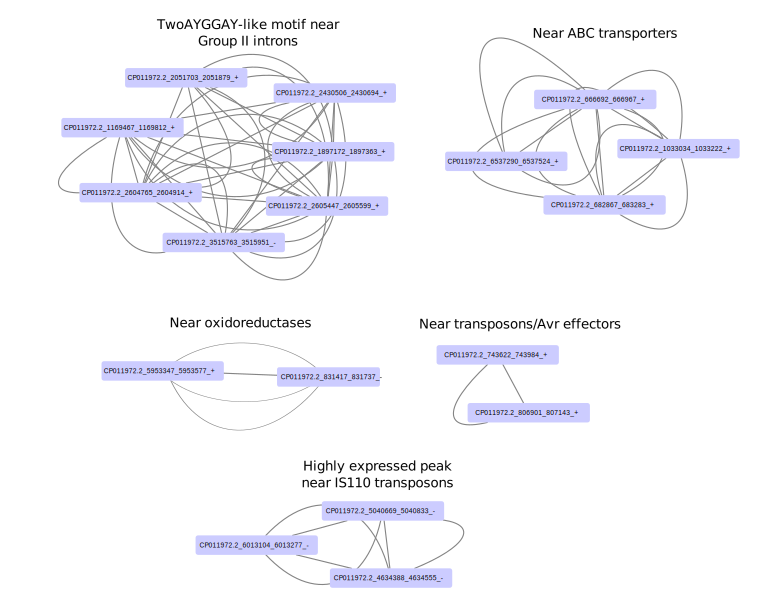
\includegraphics[scale=0.8]{psa/psa_ncRNA/all_v_all.png}
    \caption[Network diagram showing annotated ncRNAs with high sequence similarity to each other]{Network diagram showing annotated ncRNAs with high sequence similarity to each other. Networks are generated from an all vs all \texttt{blastn} search of candidate ncRNAs. Nodes are individual ncRNAs, and edges represent instances of a significant \texttt{blastn} hit to another ncRNA. Clusters are labelled based on their context in the \textit{Psa} genome and visualised in \texttt{Cytoscape} \citep{Shannon2003-uv}.}
    \label{fig:cytoscape}
\end{figure}

\subsection{Alignment analysis and structure prediction}

Several tools were used to identify alignments that were most likely to be non-coding RNAs (Figure \ref{fig:psa_flowchart}). \texttt{RNAcode} was used to test if candidate ncRNAs had protein coding potential \citep{Washietl2011x}; 20 candidates with a p value < 0.01 were removed. \texttt{Alifoldz} was used to identify alignments that had significant signals of stable secondary structure \citep{Washietl2004-pk}. Conserved candidate ncRNAs with negative z-scores were selected. For alignments with few sequences or little sequence variation, \texttt{alifoldz} z-score, \texttt{RNAalifold} secondary structures and alignments were manually inspected to select candidates.

\texttt{RNAalifold} \citep{Bernhart_Hofacker_Will_Gruber_Stadler_2008x} was used to predict a consensus secondary structure for each alignment. Six conserved candidates that did not have a thermodynamically favourable secondary structure (minimum free energy of > -20) were removed. \texttt{R-scape} \citep{Rivas_Clements_Eddy_2017x} was used to identify covarying base-pairs within predicted secondary structures. Six structures containing covarying base-pairs with an E-value < 0.01 were selected as final candidates. \texttt{R-scape} tests could not be applied to alignments with limited numbers of sequences. Thermodynamic stability and covariance scores, conservation and expression were used to select and rank the final ncRNA candidates. For candidates with limited phylogenetic distribution, MFE, overall expression and differential expression were used to select the final candidates. Secondary structures were visualised using R2R \citep{Weinberg2011-nxxx}.
\subsection{Differential gene expression and expression in other data-sets}
Candidate intergenic ncRNAs as well as Rfam annotations were tested for differential expression using \texttt{Kallisto} (settings$:$ \texttt{ -b 100 $--$rf-stranded}) \citep{Bray2016-xxoi} and DESeq2 \citep{Love2014-dccv} using the same analysis pipeline as Chapter 4 (see Appendix x for details). 

Publicly available data on the Sequence Read Archive (https://www.ncbi.nlm.nih.gov/sra) was used to find paired-end, stranded \textit{Pseudomonas} RNA-seq data-sets. Metadata from the NCBI FTP server was used to generate a table consisting of SRA accession, SRA experiment number, sequencing design (paired or single-end reads), read length, sequencing instrument, NCBI biosample, NCBI taxonomy ID, organism genome accession and species name. This table was then used to select seven \textit{P. syringae} pv. \textit{tabaci} ATCC 11528 (\textit{Pta}) transcriptomes (Table \ref{tab:tabaci_transcriptomes}, Table \ref{tab:tabaci_transcriptomes_2}), generated \textit{in vitro} in M9 media, which were used to test if candidate ncRNAs were expressed in other organisms.

Profile HMMs of candidate ncRNAs, which were generated from alignments generated during the conservation analysis, were used to annotate the \textit{Pta} genome ATCC 11528 (NCBI Accession ACHU02.1). Sequencing reads were mapped to the genome and visualised using the same pipeline as the \textit{Psa} transcriptomes (Appendix x). Homology search results were then used find sequences homologous to \textit{Psa} candidate ncRNAs in the \textit{Pta} genome that also showed similar levels of expression. 
\begin{figure}[H]
\begin{minipage}{0.6\textwidth}
    \includegraphics[scale=1]{psa/psa_ncRNA/flowchart3.png}
\end{minipage}
\begin{minipage}{0.39\textwidth}
    \caption[Flow-chart showing showing quality control steps used to select final candidate ncRNAs]{Flow-chart showing showing quality control steps used to select final candidate ncRNAs. Briefly, manual annotations that were single copy were selected for conservation analysis. Multiple sequence alignments from this homology search were then tested for signals that would identify the candidates as functional ncRNAs. \texttt{RNAcode} was used to test if sequences were likely to be protein coding \citep{Washietl2011x}, and \texttt{alifoldz} z-scores and \texttt{RNAalifold} minimum free energy (MFE) was used to identify candidates with thermodynamically stable predicted secondary structure \citep{Bernhart_Hofacker_Will_Gruber_Stadler_2008x,Washietl2004-pk}. Additional tests were placed on conserved sequences (>12 sequences) using \texttt{R-scape} \citep{Rivas_Clements_Eddy_2017x}. Manual curation removed a further 8 candidates based on poor expression and conservation, maintenance of synteny, biased sequence composition and conservation of secondary structure.}
    \label{fig:psa_flowchart}
\end{minipage}
\end{figure}




\begin{table}[H]
    \footnotesize
    \centering
    \begin{tabular}{p{3cm}cccp{6cm}}\toprule
SRA Accession &  Platform & Read length & Paired? & Experiment conditions\\\midrule
SRR3747530, SRR3747531&HiSeq 2500& 125 &Yes & M9 media, 5mM mannitol\\
SRR3747532, SRR3747533& HiSeq 2500& 125 &Yes & M9 media, 5mM mannitol, C\textsubscript{6}-HSL\\
SRR3747538, SRR3747539& HiSeq 2500& 125 &Yes & M9 media, 5mM mannitol, 3OC\textsubscript{6}-HSL\\

\bottomrule
    \end{tabular}
    \caption[\textit{Pta} transcriptomes used to validate candidate ncRNA expression (SRP078028)]{Publicly available transcriptomes from \textit{Pta} ATCC 11528 (SRP078028), used to validate expression of conserved candidate ncRNAs identified in \textit{Psa}. Data generated by \cite{Cheng2018-eo}. }
    \label{tab:tabaci_transcriptomes}
\end{table}

\begin{table}[H]
    \footnotesize
    \centering
    \begin{tabular}{p{2.5cm}cccp{6cm}}\toprule
SRA Accession &  Platform & Read length & Paired? & Experiment conditions\\\midrule
SRR3757176, SRR3757178, SRR3757179 & HiSeq 2000 & 101 & Yes & KB media, exponential/stationary phase \\
SRR3757150, SRR3757153, SRR3757154 & HiSeq 2000 & 101 & Yes & KB media, exponential phase \\
SRR3757099, SRR3757100, SRR3757106 & HiSeq 2000 & 101 & Yes & KB media, lag phase \\
\bottomrule
    \end{tabular}
    \caption[\textit{Pta} transcriptomes used to validate candidate ncRNA expression (SRP078136)]{Publicly available transcriptomes from \textit{Pta} ATCC 11528 (SRP078136), used to validate expression of conserved candidate ncRNAs identified in \textit{Psa}. Data generated by \cite{Cheng2017-ja}. }
    \label{tab:tabaci_transcriptomes_2}
\end{table}

%data was shitty !
%\begin{table}[H]
%    \footnotesize
%    \centering
%    \begin{tabular}{p{2.5cm}cccp{6cm}}\toprule
%SRA Accession &  Platform & Read length & Paired? & Experiment conditions\\\midrule
%ERR973046 & HiSeq 2000 & 102 & Yes & Swarming plates \\
%ERR973047 & HiSeq 2000 & 102 & Yes & MMR minimal media \\
%\bottomrule
%    \end{tabular}
%    \caption{Publically available transcriptomes from \textit{Pseudomonas syringae} pv. %\textit{tomato} DC3000, used to validate expression of conserved candidate ncRNAs identified in \textit{Psa}. Data generated by \cite{Nogales2015-pj}. }
%    \label{tab:tomato_transcriptomes}
%\end{table}
\section{Results and Discussion}

Manual annotation identified 94 intergenic and 137 antisense expression peaks as candidate ncRNAs. Rfam-guided annotations of known ncRNAs identified gene boundaries for 54 small ncRNAs, as well as a class of 46 ncRNA sequences with twoAYGGAY-like motifs. Rfam domains were also used to identify 56 group II intron-derived sequences, although it is unclear what proportion of these remain intact or functional.

\subsection{TwoAYGGAY-like motifs in \textit{Psa} and \textit{Pseudomonas}}

Seven intergenic peaks annotated as novel ncRNAs were identified near group II introns. These sequences had high sequence similarity to each other, Rfam-annotated twoAYGGAY motifs, as well as intergenic regions which were not expressed in this experiment. Overall 43 motifs were annotated$:$ Rfam identified 12 motifs, which increased to 36 after removing the --cut-ga thresholding during annotation (E-value threshold = 0.01). Others were identified by an nhmmer homology search, using a HMM generated from an alignment of manually annotated twoAYGGAY-like sequences. An alignment of all twoAYGGAY and twoAYGGAY-like sequences had a highly stable Y-shaped predicted secondary structure, which is similar to the Rfam twoAYGGAY motif (Figure \ref{fig:twoAYGGAY_genomic}). Motif-containing sequences within the \textit{Psa} genome are generally highly similar, and have covarying sites maintaining secondary structure.   

\begin{figure}[H]
    \centering
    \includegraphics[scale=1.25]{psa/psa_ncRNA/multi-twoayggay.png}
    \caption[Consensus predicted secondary structure of twoAYGGAY-like candidate ncRNAs, and example of tandem twoAYGGAY-motifs in \textit{Psa}]{\textbf{(A)} Consensus predicted secondary structure of candidate ncRNAs homologous to annotated twoAYGGAY ncRNAs in the \textit{Psa} genome. Candidates were aligned using \texttt{mafft-qinsi} and consensus secondary structure predicted with \texttt{RNAalifold}. \textbf{(B)} Example showing tandem repeats of the twoAYGGAY-like motif in \textit{Psa}. Bottom panel shows genome annotations. \textbf{Pink:} Motifs, \textbf{Green:} Annotated group II intron, \textbf{Blue:}  Protein annotations. Top panel shows RNA-seq counts for \textit{in vitro} and \textit{in planta} data-sets. A set of 4 tandem repeats can be seen on the forward strand at the 5$\textprime$ end of the group II intron, and a single motif at the 3$\textprime$ end. Motif annotations closest to the ends of the group II intron are palindromic, generating annotations on each strand. Annotations were visualised in the Artemis genome browser.}
    \label{fig:twoAYGGAY_genomic}
\end{figure}

The \textit{Psa} twoAYGGAY-like sequences do not have the 5$\textprime$-AYGGAY-3$\textprime$ sequence in the terminal loops, but do contain 5$\textprime$-GGA-3$\textprime$ motifs, which is consistent with the binding site of Csr/Rsm-binding RNAs \citep{Gardner2015-co}. TwoAYGGAY-like motifs were commonly found throughout the \textit{Psa} genome in intergenic regions, often near group II introns. Several intergenic regions have tandem repeats of this motif, and 26 sequences were sufficiently palindromic that they were annotated in the same location on both strands.  

Conservation analysis of the most highly expressed sequence which contained the twoAYGGAY-like motif (CP011972.2, 1897172-1897363) found that this sequence is highly conserved throughout \textit{Pseudomonas} genomes. Consensus secondary structure of sequences from the homology search is generally similar to the Rfam twoAYGGAY predicted secondary structure, but has a shorter and more variable P1 stem, a shorter P2 stem, small unpaired bulges, and a 5$\textprime$-AUGGAU-3$\textprime$
motif in the terminal loops (Figure \ref{fig:twoAYGGAY_conserved}). 

\begin{figure}[H]
    \centering
    \includegraphics[scale=0.4]{psa/psa_ncRNA/TwoAYYGAY_example.png}
    \caption[Comparison of predicted consensus secondary structure of twoAYGGAY-like motifs and the Rfam twoAYGGAY motif]{\textbf{Left:} Predicted consensus secondary structure of twoAYGGAY-like motifs in \textit{Pseudomonas} genomes. An alignment was generated by an iterative nhmmer homology search from a single twoAYGGAY-like sequence over Pseudomonas genomes. \textbf{Right:} Rfam consensus secondary structure for the twoAYGGAY motif.}
    \label{fig:twoAYGGAY_conserved}
\end{figure}

The function of these motifs are unclear, although the conservation of secondary structure and Csr/Rsm binding motif suggests they may function in the sequestration of Csr/Rsm RNA-binding proteins \citep{Gardner2015-co}. These motifs were also associated with group II introns (p = 0.008, Fisher's exact test, Table \ref{tab:fisher}). 

Group II introns have been observed to insert near palindromic motifs in \textit{P. putida} KT2440 \citep{Yeo2001-gg}, and similar palindromic elements, including ncRNAs, are often insertion sites for other mobile genetic elements \citep{Darmon2014-dxj,Dai2002-fm}. It may be that this sequence is associated with the re-homing of introns, however, the mechanisms of re-homing and transposition of bacterial group II introns are diverse and not well understood \citep{Dai2002-fm}, and their recognition sites are highly variable \citep{Lambowitz2011-oq}.
\begin{table}[H]
    \centering
    \begin{tabular}{c|cc}

         & TwoAYGGAY & Group II intron \\
        \midrule
         Adjacent & 28 & 21\\
         Independent & 15 & 35\\

         Total & 43 & 56 \\

    \end{tabular}
    \caption[Contingency table showing the association of twoAYGGAY-motifs with group II introns]{Contingency table showing the association of twoAYGGAY-motifs with group II introns. These are classified into 'adjacent', where a twoAYGGAY annotation is in an intergenic region up- or down-stream of a group II intron, and 'independent' where flanking gene annotations are not part of group II introns. For regions containing multiple clustered twoAYGGAY repeats, all repeats in the same intergenic region are classed as adjacent or independent.}
    \label{tab:fisher}
\end{table}


%Previous studies of Group II intron transposition in \textit{P. putida} found that intron transposition often ocurred next to hairpin loops, which were later identified as repetitive extragenic palindromic (REP) elements \citep{Aranda-Olmedo2002-zoc}. Several sequence regions in the \textit{Psa} TwoAYGGAY-like motifs contain the GCGGG..CCCGC sequence common to the \textit{P. putida} REP motifs \citep{Yeo2001-gg}.
%The previous observation of insertion event near the Csr-binding ncRNA \textit{rsmZ} in \textit{P. putida} KT2440 \citep{Joardar2005-uj} suggests that insertion near
\subsection{Intergenic candidate ncRNAs}

Overall 71 annotated intergenic candidates were selected for conservation analysis. Quality control of the final alignments of homologous sequences removed 21 candidates that had predicted protein coding potential, 26 conserved ncRNAs with a positive \texttt{alifoldz} z-score, and 7 candidates that did not have thermodynamically stable predicted secondary structures. In total, 36 candidate ncRNAs passed alignment quality control. The conservation of these sequences and preservation of synteny was used to attempt to classify gene origins. During manual curation 4 candidates were classed as pseudogenes due to homology with proteins and tRNAs in other genomes and were removed, and another 4 were removed due to inconsistent conservation of secondary structure. 

Most candidate ncRNAs were poorly conserved; 7 were specific to \textit{Psa}, and another 7 associated with mobile genetic elements were primarily found in {Psa} with a small number of annotations to sequences near the same MGEs present in other species. Many poorly conserved candidates were located in regions created by recent re-arrangements in the \textit{P. syringae} or \textit{Psa} lineages. Several of these had highly stable predicted secondary structures, however these were part of highly repetitive and palindromic intergenic regions, which may be remnants of previous transposition events. While rearrangements can cause the creation of novel transcripts, it is difficult to identify if these are functional ncRNAs or transcriptional noise \citep{Jose2019-xxxu}. Other poorly conserved candidate ncRNAs were associated with mobile genetic elements such as transposons and integrases, reiterating results from the conservation analysis of \textit{Salmonella} sRNAs in Chapter 3. 

\begin{table}[H]
    \footnotesize
    \centering
    \begin{tabular}{ccccc}\toprule
Name &  Sequence & Start & End & Strand\\\midrule
Psa_sRNA_003 & CP011973.1 & 21610 & 21774 & -\\
Psa_sRNA_004* & CP011973.1 & 61084 & 61315 & -\\
Psa_sRNA_005* & CP011973.1 & 61080 & 61307 & +\\
Psa_sRNA_006 & CP011972.2 & 170583 & 170708 & -\\
Psa_sRNA_007* & CP011972.2 & 806901 & 807143 & +\\
Psa_sRNA_009 & CP011972.2 & 6082989 & 6083300 & -\\
Psa_sRNA_010* & CP011972.2 & 6513384 & 6513635 & -\\
Psa_sRNA_011 & CP011972.2 & 743622 & 743984 & +\\
Psa_sRNA_012 & CP011972.2 & 3765999 & 3766298 & -\\
Psa_sRNA_013* & CP011972.2 & 1752191 & 1752476 & +\\
Psa_sRNA_014 & CP011972.2 & 3260267 & 3260449 & +\\
Psa_sRNA_015 & CP011972.2 & 739233 & 739548 & -\\
Psa_sRNA_016 & CP011972.2 & 760028 & 760267 & +\\
Psa_sRNA_017 & CP011972.2 & 2294607 & 2294819 & -\\
Psa_sRNA_018 & CP011972.2 & 5148068 & 5148376 & +\\
Psa_sRNA_019 & CP011972.2 & 768152 & 768370 & +\\
Psa_sRNA_020* & CP011972.2 & 2035568 & 2035765 & +\\
Psa_sRNA_021* & CP011972.2 & 119433 & 119810 & +\\
Psa_sRNA_022 & CP011972.2 & 119724 & 119882 & -\\
Psa_sRNA_023 & CP011972.2 & 1494687 & 1495064 & -\\
Psa_sRNA_024* & CP011972.2 & 4634388 & 4634555 & -\\
Psa_sRNA_025* & CP011972.2 & 5040669 & 5040833 & -\\
Psa_sRNA_026$\dagger$ & CP011972.2 & 1300899 & 1301216 & -\\
Psa_sRNA_027* & CP011972.2 & 745275 & 745542 & -\\
Psa_sRNA_028*$\dagger$ & CP011972.2 & 322030 & 322306 & +\\
Psa_sRNA_029* & CP011972.2 & 5438181 & 5438417 & -\\
Psa_sRNA_031$\dagger$ & CP011972.2 & 5459360 & 5459656 & +\\
Psa_sRNA_032$\dagger$ & CP011972.2 & 5469984 & 5470208 & +\\
\bottomrule
    \end{tabular}
    \caption[Genome locations of final candidate ncRNAs]{Final candidate ncRNAs and genome locations. \textbf{*} indicates that this transcript is either adjacent to or part of a mobile genetic element. \textbf{$\dagger$} denotes candidates that were found to be expressed in \textit{Pta}.}
    \label{tab:final_canditates}
\end{table}
Final candidates (Table \ref{tab:final_canditates}) were ranked by conservation, overall expression, expression in other data-sets, the presence of condition-specific expression and differential expression (Figure \ref{fig:candidate_heatmap}). Three were expressed only \textit{in vitro}, four were only expressed \textit{in planta}, two in minimal media only and one in rich log samples only. One candidate Psa\_sRNA\_012, was significantly differentially expressed across \textit{in vitro} data-sets (P\textsubscript{adj} < 0.01). 

\begin{figure}[H]
    \centering
    \includegraphics[scale=0.95]{psa/psa_ncRNA/final_candidates_heatmap2.png}
    \caption[Sequence conservation and expression of candidate ncRNAs]{Heatmap showing the annotation range and sequence conservation of intergenic candidate ncRNAs annotated in \textit{Psa} across \textit{Pseudomonas} genomes. Sequence conservation is shown as a colour gradient from blue (100\%) to red (40\%), representing genus average percent sequence identity based on alignment to the sequence from \textit{P. syringae} pv. \textit{actinidiae} ICMP 18884. Gene conservation is shown as a change in opacity, represented by the percentage of genomes with an annotation within that genus. Genes are ordered based on overall conservation. Additional panels show expression data for these genes. \textbf{Top:} Basemean from \textit{in vitro} RNA-seq calculated by DEseq2. \textbf{Middle:} Peak max of mapped reads from \textit{in planta} plot files, which is the maximum combined read depth from all \textit{in planta} plot files across the annotated region. Both panels are capped at 1000. \textbf{*} Denotes candidate ncRNAs located in the \textit{Psa} ICMP 1884 plasmid, \textbf{$\dagger$} denotes candidates that are differentially expressed \textit{in vitro}}
    \label{fig:candidate_heatmap}
\end{figure}
\newpage

Candidates that were associated with mobile genetic elements were in general more highly expressed in starvation conditions. High expression of the protein components of these MGEs was also observed in the same conditions (Chapter 4), indicating these transcripts may be under the same regulatory mechanisms. 

Psa\_sRNA\_022 was highly expressed under starvation conditions and \textit{in planta}, and found next to a hypothetical protein. Additional annotation of this hypothetical protein found homology to the Abi$/$CAAX family of transmembrane metalloproteases \citep{Kjos2010-yq}, which are involved in self-immunity to bacteriocins, and have been found as part of a cassette of resistance genes carried by toxin-antitoxin systems in \textit{Staphylococcus} \citep{Bukowski2017-gd}.  A small expression peak adjacent to this candidate was also detected. Annotations in strains outside \textit{Psa} found that Psa\_sRNA\_022 was located at the 5$\textprime$ end of a CAAX protease. This locus appears to have been disrupted in \textit{P. syringae} due to an integration or transposition event (Figure \ref{fig:srna_022_operon}). This transcript had a conserved secondary structure with a GNRA tetraloop, which are structural motifs that can form and stabilise tertiary structure \citep{Fiore2013-mf}. 

 \hfill
\begin{figure}[H]
    \centering
    \includegraphics[scale=1.5]{psa/psa_ncRNA/sRNA_022.png}
        \caption[Comparison of the Psa\_sRNA\_022 locus in \textit{Psa} and \textit{P. rhizophaerae}]{Comparison of the region containing Psa_sRNA_022 sequence in \textit{Psa} and a homologous sequence in \textit{P. rhizosphaerae} strain DSM 16299. \textbf{Top:} \textit{P. rhizosphaerae} locus containing Psa\_sRNA\_022 (blue), next to a CAAX protease. \textbf{Bottom:} \textit{Psa} locus containing Psa\_sRNA\_022, which is located between two hypothetical proteins (yellow) with homology to CAAX protease. }
    \label{fig:srna_022_operon}
\end{figure}
\begin{figure}[H]
\begin{subfigure}{0.49\textwidth}
\includegraphics[scale=0.7]{psa/psa_ncRNA/psa_srna_022_exp.png} 
\end{subfigure}
\begin{minipage}{0.49\textwidth}
\includegraphics[scale=0.8]{psa/psa_ncRNA/sRNA_022_structure.png}
    \caption[Expression and predicted consensus secondary structure of Psa\_sRNA\_022]{\textbf{Left:} Expression peak for Psa\_sRNA\_022. This region is highly expressed in starvation conditions \textit{in vitro} and is expressed \textit{in planta}. \textbf{Right:} Predicted consensus secondary structure for Psa\_sRNA\_022.}
    \label{fig:srna_022}
    \end{minipage}
\end{figure}

Psa\_sRNA\_032, located downstream of a plasmid partitioning protein ParA and conjugation machinery, was highly constitutively expressed in \textit{Psa} and all \textit{Pta} samples (Figure \ref{fig:srna_032}). This candidate was found primarily in \textit{P. syringae} pv. \textit{actinidiae}, and was homologous to intergenic regions near mobile genetic elements in 3 genomes outside of \textit{P. syringae}. This transcript appears to have a stable secondary structure, containing conserved stem-loops (Figure \ref{fig:srna_032}). The context and high constitutive expression of this transcript suggests it may be a regulator or part of a Par plasmid-maintaining toxin-antitoxin system \citep{Muthuramalingam2019-uy}.

\begin{figure}[H]
\centering
    \includegraphics[scale=1.05]{psa/psa_ncRNA/tabaci_and_psa.png}
    \begin{minipage}{0.6\textwidth}
\includegraphics[scale=0.9]{psa/psa_ncRNA/sRNA_032.png}
    \end{minipage}
    \begin{minipage}{0.39\textwidth}
    \caption[Expression of a Psa\_sRNA\_032 in \textit{Psa} and \textit{Pta}]{\textbf{Top:} Expression of Psa\_sRNA\_032 in \textit{Psa} and expression of a homologous sequence in \textit{Pta}. Psa\_sRNA\_032, which is in a locus that is conserved in both genomes is highly constitutively expressed in \textit{Psa} grown \textit{in vitro} and \textit{in planta} (\textbf{left}), and also expressed in two data-sets of \textit{Pta} grown \textit{in vitro} (\textbf{right}). Peaks are smaller in \textit{Pta} due to variations in read depth between data-sets. \textbf{Bottom:} Predicted consensus secondary structure for Psa\_sRNA\_032.}
    \label{fig:srna_032}
    \end{minipage}
\end{figure}

Psa\_sRNA\_006, which is weakly expressed \textit{in vitro} and \textit{in planta}, was found in multiple Pseudomonas species and had a highly conserved secondary structure (Figure \ref{fig:srna_006}), containing two GNRA tetraloops and a highly significant covarying base-pair (E-value = 0.0003). This candidate was located near siderophore export channels in \textit{Psa}, and was homologous to a horizontally-acquired region in \textit{P. aeruginosa} near the type IV pili regulator \textit{hrpB}. 

\begin{figure}[H]
\begin{subfigure}{0.4\textwidth}
\includegraphics[scale=0.67]{psa/psa_ncRNA/psa_srna_006_exp.png} 
\end{subfigure}
\begin{minipage}{0.59\textwidth}
\includegraphics[scale=0.9]{psa/psa_ncRNA/srna_006.png}
    \caption[Expression and predicted consensus secondary structure of Psa\_sRNA\_006]{\textbf{Left:} Expression peak for Psa\_sRNA\_006. This region is weakly expressed \textit{in planta}. \textbf{Right:} Predicted consensus secondary structure for Psa\_sRNA\_006, showing highly conserved stem-loops, containing covarying base-pairs.}
    \label{fig:srna_006}
    \end{minipage}
\end{figure}

Psa\_sRNA\_026 was conserved throughout \textit{P. syringae} and found in several closely related Pseudomonas species. This candidate was only expressed in minimal media \textit{in vitro} and was highly expressed \textit{in planta}, and is located in a conserved intergenic region located upstream of alginate biosynthesis genes, and next to a metal-sensing peroxide stress protein YaaA \citep{Liu2011-rz}. The predicted consensus secondary structure for Psa\_sRNA\_026 was highly structured, however several peripheral stem-loops were not highly conserved (Figure \ref{fig:srna_026}).

\begin{figure}[H]
    \centering
\includegraphics[width=0.9\linewidth]{psa/psa_ncRNA/psa_srna_026_exp.png} 
\end{figure}
\begin{figure}[H]
    \centering
\includegraphics[width=0.75\linewidth]{psa/psa_ncRNA/sRNA_026.png}
    \caption[Expression and predicted consensus secondary structure for Psa\_sRNA\_026]{\textbf{Top}: Expression of Psa\_sRNA\_026 in \textit{Psa}, where it is expressed in minimal media \textit{in vitro}, and \textit{in planta}. Expression in \textit{Pta} is also shown. \textbf{Bottom}: Predicted consensus secondary structure for Psa\_sRNA\_026.}
    \label{fig:srna_026}
\end{figure}

\subsection{Psa\_sRNA\_031 is a \textit{Pseudomonas syringae} \textit{pesA} homologue}
Homology search results showed that Psa\_sRNA\_031 was conserved across \textit{Pseudomonas}, including several strains of \textit{P. aeruginosa}, a well-studied human pathogen and model organism. The \textit{Pseudomonas} transcriptome browser by \cite{Wurtzel_Lory_2012x} was used to identify that an intergenic region in \textit{P. aeruginosa} str. PA14 that is homologous to Psa\_sRNA\_031 was highly expressed (Figure \ref{fig:p_browser}) and has been identified as a small RNA. This transcript, named PesA (previously known as SPA0021), is located in the PAPI-4 pathogenicity island found in many pathogenic strains of \textit{P. aeruginosa}, and may act in \textit{trans} to attenuate the expression of the bacteriocin, pyocin S3 \citep{Ferrara2017-su}. PesA also improves survival and stress tolerance in response to UV, however the mechanism for this is unclear \citep{Ferrara2017-su}. 

\begin{figure}[H]
    \centering
    \includegraphics[scale=0.8]{psa/psa_ncRNA/pseudomonas_browser.png}
    \caption[Expression of a Psa\_sRNA\_031 homologue in \textit{P. aeruginosa}] {Data from the Pseudomonas RNA-seq browser \citep{Wurtzel_Lory_2012x}), showing expression of a region homologous to Psa\_sRNA\_031 the in \textit{P. aeruginosa} str. PA14 (PA14\_sr\_128). This region overlaps with the annotated sRNA \textit{pesA}, located at 5288100-5288500 in this genome \citep{Pita2018-bi}. The Pseudomonas RNA-seq browser is located at $http://www.weizmann.ac.il/molgen/Sorek/pseudomonas\_browser/$ }
    \label{fig:p_browser}
\end{figure}

The expression of \textit{pesA} appears to be regulated differently in \textit{P. syringae} strains than in \textit{P. aeruginosa}. PesA expression is induced at body temperature in \textit{P. aeruginosa}, however it is constitutively expressed across the \textit{Psa} and \textit{Pta} RNA-seq data-sets used in this study. 

Conservation analysis and structural prediction showed that both the nucleotide sequence and secondary structure of PesA are conserved across \textit{Pseudomonas} genomes (Figure \ref{fig:pesa_structure}), with an average sequence identity of 89\% and lowest sequence identity of 71\% between \textit{Psa} and \textit{P. protogens} sequences. A sequence region of \textit{pesA} that has been predicted to be the interaction site with the pyocin S3 mRNA ribosomal binding site in \textit{P. aeruginosa} (UUCUCCCUGUGUCUCCCUGUUCUUUUGCUUGUC) was conserved across all sequences, with some variability in the 3$\textprime$ end (Figures \ref{fig:pesa_structure} and \ref{fig:pesa_binding_site}). 

\begin{figure}[H]
    \centering
    \includegraphics[scale=1.8]{psa/psa_ncRNA/Pesa_binding_site.png}
    \caption[Predicted consensus structure of PesA]{Predicted consensus structure of PesA with the experimentally confirmed mRNA binding region from \textit{P. aeruginosa} highlighted (yellow).}
    \label{fig:pesa_structure}
\end{figure}

In \textit{P. aeruginosa} and \textit{P. protegens}, \textit{pesA} is found next to genes encoding Type IV pili, however in  \textit{P. syringae} and other \textit{Pseudomonas} plant pathogens (\textit{P. avenellae}, \textit{P. amygdali} and \textit{P. cerasicola}) \textit{pesA} is located next to a DNA topoisomerase III in PacICE1, a integrative conjugative element circulating among \textit{Pseudomonas} in the Pacific \citep{Colombi2017-zf,Colombi2017-yxxf}. 
%Pacific-specific ICE 5410644	5511601 in CP011972.2
\begin{figure}[H]
\includegraphics[scale=0.9]{psa/psa_ncRNA/PesA_binding_site_conservation_2.png}
    \caption[Sequence logo showing nucleotide conservation across the PesA binding site]{Sequence logo showing nucleotide conservation across the PesA binding site. Image generated by WebLogo (https$:$//weblogo.berkeley.edu/logo.cgi)}
    \label{fig:pesa_binding_site}
\end{figure}


\begin{wrapfigure}{l}{0.5\textwidth}
\centering
    \includegraphics[scale=0.72]{psa/psa_ncRNA/pesa_iyo_017970.png}
    \caption[CopraRNA predicted interaction between Psa\_sRNA\_031 and IYO\_017970]{Visualisation showing the top predicted interaction between Psa\_sRNA\_031 (\textit{pesA}) and \textit{Psa} mRNAs generated by CopraRNA \citep{Wright2014-vh,Wright2013-cc}. Interacting regions of the predicted conserved binding region of PesA and a region upstream of the start codon of IYO_017970  are shown. Figure generated with RNAplot \citep{Lorenz2011-wt}. }
    \label{fig:copraRNA}
\end{wrapfigure}To investigate if \textit{pesA} functions in pathogenicity in \textit{P. syringae}, CopraRNA \citep{Wright2014-vh,Wright2013-cc} was used to predict conserved interactions between PesA and mRNA sequences in 4 \textit{P. syringae} strains, \textit{P. syringae} pv. \textit{actinidiae} ICMP 18884 (NCBI accession: NZ\_CP011972), \textit{P. syringae} pv. \textit{syringae} B728a (NCBI accession: NC\_007005), 
\textit{P. syringae} pv. \textit{tomato} str. B13-200 (NCBI accession: NZ\_CP019871) and \textit{P. syringae} pv. \textit{atrofaciens} str. LMG5095 (NCBI accession: NZ\_CP028490). CopraRNA high scoring interactions (Table \ref{tab:COPRARNA}) include stress genes that are required for survival \textit{in planta}, indicating that PesA may have an analogous role in promoting survival in plant hosts. The top-scoring interaction with an arylesterase, an enzyme which is involved in the degradation of carboxylic and phenolic esters \citep{Wang2010-fs}, which are present in many plant-derived compounds such as salicyclic acid and lignin. Phenolic compounds have been shown to induce the expression of \textit{hrp} virulence and T3SS genes in \textit{P. syringae} pv. \textit{tomato} \citep{Lee2015-ub}. The ArnA interaction with PesA was predicted to interact with the previously identified PesA binding site (Figure \ref{fig:copraRNA}). Other targes include UDP-glucoronic acid oxidase ArnA, which is involved in LPS synthesis \citep{Breazeale2002-cd}, and PhnA, which is involved in the uptake of alkylphosphonates, which are phosphate-containing compounds that include some fungicides and herbicides \citep{Chen1990-ql}. Other targets include the ribosomal protein RpsO, which binds to the 16S RNA and has been found to interact with sRNAs in \textit{E. coli} \citep{Fontaine2016-go}, and UspA, which is a conserved components of many stress responses \citep{Kvint2003-kg}.

%Describe how copraRNA works

%\begin{figure}[H]
%    \centering
%    \includegraphics[scale=0.7]{psa/psa_ncRNA/PesA_sRNA_regions_with_histogram.pn}
%    \caption{Histogram of predicted interaction regions of the \textit{P. syringae pesA} homologues with mRNAs. The top predicted interaction is highlighted in red, which overlaps with the previously predicted pesA binding site.}
%    \label{fig:my_label}
%\end{figure}
%\begin{figure}[H]
%    \centering
%    \includegraphics[scale=0.7]{psa/psa_ncRNA/PesA_mRNA_regions_with_histogram.png}
%    \caption{Histogram of predicted interaction regions of mRNAs interacting with \textit{pesA}. For this analysis, only the region 200 nt upstream and 100 nt downstream of each mRNA was analysed. The top predicted interaction is highlighted in blue.}
%    \label{fig:my_label}
%\end{figure}

%, sRNApredict2 \citep{Cao2009-hf} was used to identify potential targets for PesA in \textit{P. syringae} pv. B728a. Three of the top-ranked results were predicted to interact with the binding site previously identified in \textit{P. aeruginosa} (Figure \ref{fig:pesa_targets}). PesA was predicted to interact immediately upstream of the start codon for two of these genes, a glutamate-ammonia lyase and a sulphonate transporter, and may bind to the ribosome binding site of these mRNAs. 
%\begin{figure}[H]
%    \centering
%    \includegraphics[scale=0.5]{psa/psa_ncRNA/pesa_targets_p_syringaeB728a.png}
%    \caption[Predicted targets of PesA in \textit{P. syringae} pv. \textit{syringae} B728a]{Predicted targets of PesA in \textit{P. syringae} pv. \textit{syringae} B728a that are predicted to interact with a previously-identified binding region. Alignments are shown between PesA and three genes. Bases from the PesA binding site are highlighted with asterisks. Predictions generated by sRNApredict2 \citep{Cao2009-hf}.}
%    \label{fig:pesa_targets}
%\end{figure}
\begin{table}[H]
    \footnotesize
    \centering
    \begin{tabular}{cccl}
\toprule
CopraRNA p-value & Gene & Energy [kcal/mol] & Functional annotation of gene\\
\midrule
9.43E-06 & IYO_017970 & -24.38 & arylesterase\\
9.63E-05 & IYO_016195 & -26.59 & UDP-glucuronic acid oxidase ArnA\\
0.000147 & IYO_022295 & -22.23 & putative RNA-binding protein\\
0.000193 & IYO_022725 & -21.15 & 30S ribosomal protein S15 rpsO\\
0.000195 & IYO_010790 & -16.45 & universal stress protein UspA \\
0.000239 & IYO_018865 & -19.45 & hydroxyacylglutathione hydrolase\\
0.000248 & IYO_021105 & -20.62 & methionine--tRNA ligase\\
0.00025 & IYO_009170 & -20.91 & Free methionine-(R)-sulfoxide reductase\\
0.000275 & IYO_014440 & -18.96 & DUF1993 domain-containing protein \\
0.000283 & IYO_023490 & -20.12 & Alkylphosphonate utilization operon protein PhnA\\
\bottomrule
    \end{tabular}
    \caption[Top 10 PesA-mRNA interactions predicted by CopraRNA]{Top 10 PesA-mRNA interactions predicted by CopraRNA. CopraRNA p-value, gene and protein annotations, and predicted thermodynamic stability of the interaction are shown.}
    \label{tab:COPRARNA}
\end{table}

%\begin{figure}
%    \centering
%    \includegraphics{psa/psa_ncRNA/pesa_copraRNA_interaction.png}
%    \caption{Caption}
%    \label{fig:my_label}
%\end{figure}

\subsection{Antisense ncRNAs}

Antisense transcription peaks were found for 137 genes (see Appendix x). Most antisense peaks were short (\textasciitilde300 nt) and had low expression relative to their counterpart genes. Antisense transcripts appear to be abundant in bacterial transcriptomes \citep{Georg2011-XXee}, however, they are often poorly conserved and few have been functionally characterised \citep{Cech2014-pxe}, leading to scepticism about what proportion of such transcripts act as functional ncRNAs \citep{Llorens-Rico2016-hvxx}.
Only 4 antisense transcripts were differentially expressed \textit{in vitro} (Table \ref{tab:antisense_sig}), which were all more highly expressed in starvation conditions and down-regulated in minimal media. 

Fifteen antisense transcripts were only expressed in specific growth conditions (Table \ref{tab:antisense_specific}). These were mostly expressed in rich media in log phase, and were antisense to several genes important for \textit{Psa} pathogenicity and survival. 

In rich media, antisense transcripts were mainly found opposite genes involved in iron metabolism, recombination and transposition. Antisense transcripts expressed in rich media in log phase were opposite genes involved in recombination and transposition, the biosynthesis of haem-containing molecules, as well as the haem-sensing TonB-dependent receptor, a membrane protein part of a lytic phage (IYO\_005850), and a lipoprotein (IYO\_003010) located next to anti-microbial peptide transporters. In rich media in log/late log phase, a transcript was found opposite a hypothetical protein, which was located in a locus containing tellurium resistance genes that may be involved in phage suppression \citep{Anantharaman2012-zj}. These may be involved in the regulation of iron homeostasis and the suppression of lytic phages and transposons.
 \hfill
\begin{table}[H]
    \footnotesize
    \centering
    \begin{tabular}{cccccp{6cm}}\toprule
Start &  End & Strand & L\textsubscript{2}FC (RvM) & L\textsubscript{2}FC (MvS) & Opposite gene\\\midrule
 2734548 & 2734968 & -	& \textbf{-1.8} & \textbf{2.0} & IYO_012460 enoyl-CoA hydratase \\
 2385543 & 2385788 & -	& \textbf{-2.9} & - & IYO_011015 GNAT family acetyltransferase \\
 4143876 & 4144167 & -	& - & \textbf{1.8} & IYO_018595 FAD-binding molybdopterin dehydrogenase \\
 4614055 & 4614566 & -	& - & \textbf{1.2} & IYO_020700 peptide ABC transporter ATP-binding protein\\
\bottomrule
    \end{tabular}
    \caption[Antisense peaks that are differentially expressed \textit{in vitro}]{Antisense peaks in the \textit{Psa} (CP011972.2) genome that are differentially expressed \textit{in vitro}. Significant log\textsubscript{2} fold changes (p < 0.01) are included for rich vs minimal and minimal vs starved media comparisons. }
    \label{tab:antisense_sig}
\end{table}

In minimal media and starved samples, antisense transcripts were found for genes involved in carbon metabolism, DNA repair and siderophore transport. In minimal media, a transcript was found opposite a glycine transporter (Figure \ref{fig:antisense_specific}). In starvation conditions, transcripts were found antisense to a transcriptional regulator of genes involved in the TCA cycle, as well as maltodextrin phosphorylase, which is involved in carbohydrate metabolism \citep{Watson1997-gq}. Starvation-specific antisense transcripts were also found for a transposon near the HopAM1-1 effector, and the DNA-repair protein mutL \citep{Ban1998-js}. 

Differentially expressed antisense transcripts were opposite genes involved in acetyl-CoA synthesis, a xanthine dehydrogenase, which contains iron-sulphur clusters, and a peptide transporter (Table \ref{tab:antisense_sig}).

The changes in expression for the annotated antisense transcripts broadly reflect changes in gene expression discussed in Chapter 4, where rich media is characterised by growth and the suppression of siderophore production, and nutrient acquisition and the pivoting of carbon metabolism to the TCA cycle in minimal media and starvation samples.

\begin{figure}[H]
    \centering
    \includegraphics[scale=1.4]{psa/psa_ncRNA/antisense_condition_specific.png}
    \caption[Examples of condition-specific antisense transcription in \textit{Psa}]{Examples of condition-specific antisense transcription in \textit{Psa}. Read depth is visualised as plot files for each strand, which are coloured according to growth condition for the sample. \textbf{Left}$:$ Antisense transcription opposite a TonB-dependent receptor (IYO\_006325) occurring only in rich media samples in log phase. \textbf{Right}$:$ Antisense transcription opposite a glycine ABC transporter (IYO\_004105) occurring only in minimal media samples.}
    \label{fig:antisense_specific}
\end{figure}
One antisense ncRNA spanning the 3$\textprime$ of \textit{ureA} gene and the 5$\textprime$ of \textit{pat} was highly expressed in \textit{Psa}, particularly under starvation conditions, and was also expressed in \textit{Pta}. A 5$\textprime$ \textit{ureB} transcript has previously been discovered in \textit{Helicobacter pylori} \citep{Wen2011-cd}, where it acts to regulate \textit{ureB} and \textit{ureA} expression in neutral pH, when the requirement for urease is reduced. Interestingly, an Rfam search annotated a region antisense to \textit{ureC} as homologous to the \textit{H. pylori} 5$\textprime$ ureB antisense RNA, however this region was not expressed under any RNA-seq conditions in this study. 
\begin{table}[H]
    \footnotesize
    \centering
\begin{tabular}{cccp{7cm}c}\toprule
Start &  End & Strand & Opposite gene & Expressed in \\\midrule
5288805 & 5289233 & - & IYO_023770	hypothetical protein & Rich late log\\
4886574 & 4887107 & - & IYO_021900	membrane protein & Rich log \\
4791323 & 4791737 & + & IYO_021485	DNA recombination protein RecO & Rich log \\
4478352 & 4479341 & - & IYO_020055	spermidine/putrescine ABC transporter ATP-binding protein/IYO_020050	ABC transporter permease & Rich log\\
4296010 & 4296513 & + & IYO_019195	RND transporter/IYO_019200 BNR/Asp-box repeat-containing protein & Rich log\\
4347701 & 4348589 & + & IYO_019435	multifunctional fatty acid oxidation complex subunit alpha	IYO_019440	hypothetical protein & Rich log\\
2522527 & 2522700 & - &  IYO_011620 sirohydrochlorin ferrochelatase & Rich log\\
1369572 & 1369895 & + & IYO_006325	TonB-dependent receptor	& Rich log\\
1245423 & 1245888 & +	& IYO_005850 membrane protein & Rich log\\
617339 & 617594 &	+ & IYO_003010 lipoprotein	& Rich log\\
864468 & 865185 & - & IYO_004105 glycine/betaine ABC transporter substrate-binding protein & Minimal\\
2403507 & 2403680 & - & IYO_011100 LacI family transcriptional regulator & Starved\\
5160963 & 5161205 & + & IYO_023220 integrase & Starved\\
5601902 & 5602174 & + & IYO_025370 DNA mismatch repair protein & Starved\\
5880993 & 5881310 & - & IYO_026510 maltodextrin phosphorylase & Starved\\
\bottomrule
    \end{tabular}
    \caption{Antisense peaks in the \textit{Psa} (CP011972.2) genome with condition-specific expression \textit{in vitro}.}
    \label{tab:antisense_specific}
\end{table}

Urease is a highly conserved protein that functions in acid stress in aerobic bacteria, and is also a marker of virulence in fluorescent Pseudomonads \citep{Bradbury2014-ij}. The operon structure for the urease sub-units are significantly different between \textit{Psa} and \textit{H. pylori} (Figure \ref{fig:ureB_operon}). In \textit{P. syringae} this locus has an insertion of two acetyltransferases; a tabtoxin-resistance protein, which acts to protect tabtoxin-producing \textit{P. syringae} strains from their own phytotoxin \citep{Wencewicz2012-dg}, and a phosphinothricin N-acetyltransferase, which reduces toxicity of phosphinothicin, a phytotoxin and common herbicide \citep{Davies2007-nb}. It is unclear if this \textit{Psa} antisense transcript has the same function as the \textit{H. pylori ureB} antisense transcript, however the \textit{pat} insertion between \textit{ureA} and \textit{ureB} is conserved across \textit{Pseudomonas} genomes (\cite{Davies2007-nb}, $http://www.pseudomonas.com/$
$orthologs/list$?$id=112598$).

\begin{figure}[H]
\centering
        \includegraphics[scale=1.2]{psa/psa_ncRNA/ureb.png}
    \caption[Urease operons in \textit{Helicobacter pylori} and \textit{Psa}]{Structure of the urease operons in \textit{Helicobacter pylori} \citep{De_Reuse1997-mz} and \textit{Psa} (based on NCBI genome annotations), showing an insertion in between the \textit{ureA} and \textit{ureB} genes in \textit{Psa}. \textbf{Blue$:$} Antisense sRNA annotations. \textbf{Red}$:$ Components of the urease operon. \textbf{Yellow$:$} Toxin-resistance acetyltransferases \textit{pat} and \textit{ttr}.}
    \label{fig:ureB_operon}
\end{figure}

\subsubsection{Antisense expression in other \textit{P. syringae} strains}
Expression of antisense peaks in \textit{Psa} were generally not conserved, as only 18/64 homologous sequences in \textit{Pta} showed expression > 50 counts across in either of the RNA-seq data-sets; only 5 of these were consistent across both data-sets. Two antisense peaks showed high expression, which were opposite a peptidase (IYO\_026530 in CP011972.2, and C1E\_0209610 in ACHU02.1) and an AraC transcriptional regulator (IYO\_019675 in CP011972.2, and C1E\_0211300 in ACHU02.1).

Antisense sRNAs have been previously been characterised in \textit{P. syringae} pv. \textit{tomato} DC3000 in the \textit{cmaU} and \textit{aefR} genes \citep{Filiatrault_2010x}, however these genes did not show antisense transcription in \textit{Psa} in this study. The most well-characterised antisense sRNA, \textit{fleQ}\textsubscript{as}, was predicted to have a conserved promoter region across Pseudomonas, including \textit{Psa} \citep{Markel2018-yz}. In \textit{P. syringae} pv. \textit{tomato} DC3000 \textit{fleQ}\textsubscript{as} was found to be dependent on AlgU expression, however antisense transcription was not detected despite consitutive AlgU expression \textit{in vitro} in \textit{Psa}. 
%FleQ is IYO\_009975
The poor conservation of antisense transcription in \textit{P. syringae} is consistent with previous observations in \textit{P. aeruginosa}, where antisense-expression was found to be strain and condition specific \citep{Gomez-Lozano2014-sh}, and with antisense transcription in general \citep{Llorens-Rico2016-hvxx}. 

Antisense transcripts for Hop effectors have previously been found in \textit{P. syringae} pv. \textit{tomato} DC3000 \citep{Filiatrault_2010x}. Several expression peaks were also found opposite Hop effectors in \textit{Psa} (Figure \ref{fig:hop_antisense}), however the \textit{Psa} and \textit{P. syringae} pv. \textit{tomato} genomes contain different cohorts of effectors.% However, as these genes are highly similar to transposons and mobile genetic elements it is difficult to determine if these peaks are the result of multi-mapping of RNA-seq reads without further validation. 

 \hfill
\begin{figure}[H]
    \includegraphics[scale=1.25]{psa/psa_ncRNA/antisense_hop.png}
    \caption[Antisense transcription to Hop effectors in \textit{Psa}]{Antisense transcription to Hop effectors in \textit{Psa}. The top two panels show read depth for \textit{in vitro} experiments for each strand, coloured by experiment type. \textbf{Green:} Rich media, \textbf{Blue:} minimal media, \textbf{Red:} starvation. \textbf{Left$:$} A short peak expressed in starvation conditions opposite HopAU1. \textbf{Middle:} A peak overlapping with the 3$\textprime$ end of HopAO2. \textbf{Right:} A highly expressed peak antisense to the 5$\textprime$ end of HopN1.}
    \label{fig:hop_antisense}
\end{figure}


\subsection{Expression of Rfam annotated ncRNAs}

In total, 50 Rfam annotated ncRNAs, excluding ribosomal RNAs, tRNAs and group II introns, were expressed \textit{in vitro}. Two ncRNAs were only expressed \textit{in planta}, and 29 ncRNAs were expressed in both \textit{in vitro} and \textit{in planta} data-sets.

The most highly expressed RNA in both \textit{in vitro} and \textit{in planta} samples was RsmY, which is part of the the Csr/Rsm family of ncRNAs. Csr/Rsm (carbon storage regulator, or repressor of secondary metabolism) is a widespread regulon of sRNAs and RNA-binding proteins that act to globally regulate metabolic pathways in response to environmental signals \citep{Duss2014-rs}. The Csr/Rsm family is comprised of a diverse set of ncRNAs, and contain GGA motifs in loops that allows them to sequester the RNA-binding proteins CsrA/RsmE. In \textit{Pseudomonas syringae}, three Rsm ncRNAs, RsmX, RsmY and RsmZ \citep{Janssen2018-fv,Moll2010-lt} are important regulators of metabolism, which are themselves under the control of the GacS/GacA two-component system \citep{Brencic2009-hn}.

Three ncRNAs annotated as CrcZ, a Csr$/$Rsm ncRNA that is a global suppressor of catabolism \citep{Filiatrault2013-us}, were among the most highly expressed ncRNAs \textit{in vitro} and \textit{in planta}. These annotations likely represent the three \textit{P. syringae} ncRNAs CrcX, CrcY and CrcZ \citep{Filiatrault2013-us}, of which only CrcZ is represented in Rfam. 

An annotation of the RMF RNA (location CP011972.2 4079040-407910), which is found in the 5$\textprime$ UTR of ribosomal modulation factors in Pseudomonas \citep{Weinberg2010-gu}, was highly expressed at the 5$\textprime$ end of a ~500 bp expression peak overlapping an open reading frame. This region is likely to contain an un-annotated rmf gene or pseudogene. Several riboswitches and cis-regulatory elements, including FMN, Cobalamin, sucA-II and rne-II were also highly expressed \textit{in vitro}. 

\subsubsection{RgsA is differentially expressed \textit{in vitro}} 
P16, also called RgsA, was the only Rfam-annotated ncRNA that was significantly differentially expressed (p\textsubscript{adj} < 0.01) \textit{in vitro}, and was up-regulated in starvation conditions. RgsA is a short Hfq-binding ncRNA that is highly expressed in stationary phase, and forms a reciprocal regulatory circuit with the RpoS sigma factor \citep{Lu2018-qy}, which is a major transcriptional regulator during stationary phase. This sRNA has been found to play a role in protection from H\textsubscript{2}O\textsubscript{2}-induced oxidative stress in \textit{P. aeruginosa}, \textit{P. fluorescens} \citep{Gonzalez2008-yl}, and in \textit{P. syringae} pv. \textit{tomato} \citep{Park2013-pb}, where it has been proposed to function in tolerance of plant defence response. RgsA also contains GGA loop motifs, suggesting it is part of the Csr/Rsm system.

\subsubsection{Condition-specific expression}

Three \textit{Pseudomonas}-specific ncRNAs, P24, PhrS and GabT, were found to be expressed only under specific growth conditions \textit{in vitro}. P24, an uncharacterised \textit{Pseudomonas} ncRNA, was expressed in minimal media in \textit{Psa}. Previously, P24 has been found to be expressed stationary phase in \textit{P. aeruginosa} \citep{Livny2006-nf}, and in minimal media in \textit{P. putida}, where it is down-regulated in response to osmotic stress \citep{Bojanovic2017-ph}.  
%pat203 in here
%https://aem.asm.org/content/aem/suppl/2017/03/08/AEM.03236-16.DCSupplemental/zam999117744s1.pdf

 \hfill
\begin{figure}[H]
    \centering
    \includegraphics[scale=0.9]{psa/psa_ncRNA/rfam_condition_specific.png}
    \caption[Condition-specific expression of Rfam annotated ncRNAs \textit{in vitro}]{Condition-specific expression of Rfam annotated ncRNAs \textit{in vitro}. \textbf{Left$:$} PhrS expressed in rich media in log phase (light green). \textbf{Middle$:$} P24 expressed in minimal media (blue). \textbf{Right$:$} gabT expressed in two samples under starvation conditions (red, bold line).}
    \label{fig:rfam_specific}
\end{figure}

The PhrS RNA, located next to a pectate lyase in \textit{Psa}, was only expressed in rich media during log phase. The PhrS RNA is involved in virulence in \textit{P. aeruginosa}, where it is expressed in response to oxygen limitation and functions to regulate quorum sensing \citep{Sonnleitner2011-jk} and CRISPR-cas systems \citep{Lin2019-ks}. However, its role in other Pseudomonads is unclear.

The gabT RNA, a \textit{Pseudomonas}-specific putative \textit{cis}-regulator of GabT (a transaminase) or GabD \citep{Weinberg2010-gu}, was only expressed in two replicates under starvation conditions (highlighted in Figure \ref{fig:rfam_specific}). GabT proteins are involved in the production of succinate from GABA, a common metabolite that also functions as a plant signalling molecule. In \textit{P. syringae} pv. \textit{tomato} DC3000, \textit{gabT} knockouts have been found to have reduced virulence.

Three ncRNAs were highly expressed \textit{in planta} during late infection (Figure \ref{fig:rfam_120}). This late stage of infection is characterised the upregulation of genes involved in nutrient acquisition as well as genes involved in the production of alginate and biofilms \citep{McAtee_2018x}. 

The guanidine-I riboswitch ykkC-yxkD, was only expressed \textit{in planta} at the 120hr time-point post-infection. This riboswitch binds selectively to guanidine, a product of arginine and guanine degradation, which is toxic to the cell \citep{Nelson2017-lz}. YkkC-yxkD is located upstream of urea carboyxlase transport genes in \textit{Psa}, which have previously been found to selectively transport guanidine \citep{Nelson2017-lz}. 

 \hfill
\begin{figure}[H]
    \centering
    \includegraphics[scale=0.9]{psa/psa_ncRNA/rfam_120hrs.png}
    \caption[Condition-specific expression of Rfam-annotated ncRNAs \textit{in planta}]{Condition-specific expression of Rfam-annotated ncRNAs \textit{in planta}. Three ncRNAs, ykkC-yxkD, RsmZ/PrrB and P15 all show high expression 120 hours post-infection relative to other time-points. This can be seen as a black trace representing the sum across three replicates at this time-point. YkkC-yxkD and RsmZ/PrrB appear to be specifically expressed at this time-point \textit{in planta}, whereas P15 is also expressed across all \textit{in vitro} samples. }
    \label{fig:rfam_120}
\end{figure}
\newpage
The P15 RNA, a \textit{Pseudomonas}-specific sRNA with unknown function that has previously been identified as being expressed in stationary and exponential phase in \textit{P. aeruginosa}, was highly expressed at 120hrs post infection relative to other \textit{in planta} samples, and was also expressed \textit{in vitro}.

The RsmZ sRNA (also called PrrB), a protein-sponge capable of sequestering up to multiple RsmE dimers per transcript \citep{Duss2014-rs}, was also only expressed \textit{in planta} at 120hrs post-infection. RsmZ expression is induced by GacA, a response regulator with widespread and variable roles in virulence in \textit{P. syringae} strains \citep{Chatterjee2003-ri}. Although RsmX, RsmY and RsmZ are all under the same regulatory control mechanism and appear to be functionally redundant \citep{Moll2010-lt}, RsmX and RsmY were expressed across all samples, whereas RsmZ was late infection-specific. This reflects previous observations of a fine-tuned regulatory cascade in \textit{P. fluorescens} \citep{Kay2005-gv}. \cite{Kay2005-gv} proposed that the presence of multiple redundant sRNA genes may be part of a gene dosage mechanism to allow the fine-tuning of the Gac/Rsm cascade. This regulon appears to be expanded in \textit{P. syringae} pathovars, which have up to five copies of RsmX \citep{Moll2010-lt}. In \textit{Psa}, the four copies of RsmX each showed different levels of expression relative to each other, which appears to support this hypothesis.

\section{Conclusions and future directions}

Bacterial ncRNAs are important components of gene regulation, however they are generally poorly conserved. We have performed comparative RNA-seq to identify expressed intergenic regions, and used computational measures of sequence and structural conservation to predict potential candidate ncRNAs. 

Several of the candidates we identified were present on mobile genetic elements, including a plasmid and integrative conjugative element. \textit{P. syringae} genomes are highly variable, and host to a diverse population of mobile genetic elements and plasmids \citep{Bardaji2011-jc,Gutierrez-Barranquero2017-id, Colombi2017-yxxf}. This is also true for \textit{Psa} genomes, which has a large accessory genome \citep{McCann2017-xjvkhy}.

This exchange of genetic material plays an important role in pathogenicity via the transfer of virulence genes \citep{Melnyk2019-lx}, and by introducing structural changes due to their mobilisation \citep{Jackson2011-vd,Baltrus2017-xjkkk}. The frequent conjugation and population of diverse mobile genetic elements circulating in environmental \textit{Pseudomonads} are likely to introduce new ncRNAs at a high rate, and may require sampling of multiple strains within a species or population to identify ncRNAs in the accessory genome.

We have identified 27 candidate ncRNAs that are expressed in \textit{Psa} in infection-relevant conditions, including 6 transcripts which are expressed in other pseudomonads. We have also explored the expression of known ncRNAs families in \textit{Psa}. During candidate annotation we identified a twoAYGGAY-like motif, often associated with group II introns, that are abundant in \textit{Pseudomonas} genomes. These motifs, some of which and are transcribed, appear to be Csr/Rsm-binding, however their function as transcripts or genomic elements is unclear. Work is planned with collaborators at the Plant and Food Research Centre, Auckland, to experimentally validate candidate intergenic ncRNAs identified in this study. This will include verification of the transcripts, knock-outs and fitness assays to identify if candidate ncRNAs are important for growth or pathogenicity.

\bibliographystyle{otago}
\bibliography{psa_ncRNA}
\cleardoublepage
\chapter{Genome assembly of \textit{Gemmata} isolates}
\label{chap:assembly}

\section{Preface}
This chapter and appendix x briefly describe my work on two genome sequencing projects during my time at the University of Canterbury. This work describes the genome assembly and preliminary analysis of \textit{Gemmata} isolates, as part of a collaboration with Paul Gardner, Amy Osborne and Anthony Poole. This builds on previous work in this group, which explored the relationship between expression of ncRNAs and phylogenetic distance, which concluded that phylogeny-informed sampling is required for comparative methods to be effective. For this project, outgroups in the 'goldilocks zone', i.e phyla at a specific distance that will allow transcriptomic comparison, including \textit{Gemmata}, have been selected for sequencing. 

\section{Contributions}
I performed all assembly and data analysis. Isolates were grown and prepared for sequencing by Amy Osborne.
\newpage
\section{Introduction}

\textit{Gemmata} are a genus of aerobic budding bacteria found in freshwater and in soil, which is of particular interest in evolutionary biology due to their phenotypic similarity to eukaryotes and archaea \citep{Franzmann1984-ms,Devos2013-ds}. \textit{Gemmata} are part of the Planctomycetes superphylum, which are a widespread group of environmental bacteria with unusual phenotypic and physiological characteristics reminiscent of eukaryotic cell. An especially noteable feature of planctomycetes is the presence of intracellular compartments \citep{Lindsay2001-qg}, including a large compartment enclosing the nucleoid that has been found in \textit{Gemmata obscuriglobus} (Figure \ref{fig:gemmata_cell}) \citep{Fuerst2005-kx}. 

\begin{figure}[H]
    \begin{minipage}{0.7\textwidth}
    \includegraphics[scale=0.7]{assembly/gemmata_cell.png}
    \end{minipage}
    \begin{minipage}{0.29\textwidth}
    \caption[Diagram showing the intracellular compartments of a \textit{Gemmata obscuriglobus} cell]{Diagram showing the intracellular compartments of a \textit{Gemmata obscuriglobus} cell. Adapted from \cite{Fuerst2011-le}.}
    \label{fig:gemmata_cell}
    \end{minipage}
\end{figure}

The taxonomic placement of planctomycetes has been debated, as they share phenotypic features with eukaryotes, such as reproduction \textit{via} yeast-like budding of the extracellular membrane, and also contain ammonia metabolic pathways normally found in archaea \citep{Fuchsman2006-zz,Fuerst2011-le}. \textit{Gemmata obscuriglobus} also has the unusual ability produce sterols \citep{Rivas-Marin2019-jd}, and utilises an endocytosis-like system for protein uptake \citep{Lonhienne2010-qa}.

However, there is some debate as to whether these features are structurally analagous rather than due to some shared homology \citep{McInerney2011-bx}. Planctomycetes have no substantial shared gene content with other kingdoms, aside from some small amount presumably obtained by HGT \citep{Fuchsman2006-zz}.

Currently, only a handful of representative strains and genome sequences are available for \textit{Planctomycetes}, with \textit{G. obscuriglobus} being the sole sequenced representative of the genus \textit{Gemmata}. We have sequenced and annotated the genomes of a strain of \textit{G. obscuriglobus}, and 4 other \textit{Gemmata}-like isolates as part of an effort to increase the number of genomes available for comparison for this under-sampled bacterial phyla \citep{Wu2009-zh}. 
This chapter describes the assembly, annotation and a preliminary comparative analysis of these genomes, which found large numbers of transposons in \textit{G. obscuriglobus}, and high levels of rearrangements across the clade.

\section{Methods}

\subsection{Sequencing}
\textit{Gemmata} isolates were collected from Queensland, Australia. \textit{Gemmata}-like str. JW3-9s0 (aka Soil9) and \textit{Gemmata obscuriglobus} were isolated from soil, \textit{Gemmata}-like str. CJuq14 and \textit{Gemmata}-like str. JW9-3f1 from a eutrophic lake and \textit{Gemmata}-like str. JW11-2f5 from an ornamental fountain. Isolates were previously classified as Gemmata-like based on phylogenetic analysis of 16S sequences \citep{Wang2002-qh}. Samples were isolated, cultured and prepared for sequencing as described in \citep{Wang2002-qh}. The genomes of all isolates were sequenced using Pacific Biosciences SMRT$\textsuperscript{TM}$ sequencing. 

\subsection{Assembly and analysis}

Raw bas.h5 files were converted to fastq reads with bash5tools.py from the pbh5tools package from PacificBiosciences (https://github.com/PacificBiosciences/pbh5tools/). Reads were trimmed and assembled using Canu v1.5 (default settings) \citep{Koren2017-fv}. Genomes were circularised with Circlator \citep{Hunt2015-tj}. Reads were mapped to the genome assemblies using BLASR \citep{Chaisson2012-sx} to generate alignments for Qualimap, which was used to assess coverage and quality of the assemblies \citep{Okonechnikov2016-ly}. Genome assemblies were annotated with Prokka \citep{Seemann2014-sxxa}. To improve gene annotations, a custom database of planctomycetes protein annotations was used as an additional reference, consisting of all protein annotations of plantomycete genomes from NCBI. The gram negative option for identifying signal peptides was used during annotation, as genes involved in outer membrane biogenesis have previously been identified in \textit{Planctomycetes} \citep{Speth2012-of}. Whole genome alignments were performed using mauve genome aligner \citep{Darling2010-vl}. Roary was used to identify the number of orthologous genes between the isolates \citep{Page2015-lu}. 

\section{Results and Discussion}

The genome assembly tools completely resolved two genomes, \textit{G. obscuriglobus} UQM2246 and \textit{Gemmata}-like str. JW11, and generated large high-coverage contigs for other strains (Table \ref{tab:genome_stats}). The genome sizes ranged between 7.86--10.14 Mb, with high \% GC content (64--70\%), which is consistent with the genomes of other \textit{Gemmata} and \textit{Planctomycete} genomes \citep{Franke2018-ys}. A small contig in the \textit{Gemmata}-like str. CJuql4 assembly was classed as a plasmid by Circlator. Plasmid-encoded RepA proteins were annotated in larger contigs in Gemmata-like str. JW9 and Gemmata-like str. JW3-8s0, indicating that plasmid reads may have been mis-assembled into genome contigs. CRISPR-cas casettes were also detected in all assemblies except \textit{Gemmata}-like str. JW9, however \textit{cas} endonucleases were found in all genome assemblies (Table \ref{tab:annotation_stats}).

\begin{table}[H]
    \footnotesize
    \centering
\begin{tabular}{rcccccc}\toprule
Strain & Genome Contigs & Size (Mb) & \% GC &
Circular & Plasmid contigs & Mean coverage (X)\\
\midrule
UQM2246 & 1 & 8.99 & 67.36 & Yes & 0 & 106  \\
JW3-8s0 & 1 & 10.14 & 63.95 &  No & 0 & 91\\
CJuql4 & 3 & 7.94 & 69.87 & No & 1 & 109\\
JW11 & 1 & 8.86 &  68.71 & Yes & 0 & 91\\
JW9 & 5 & 10.03 & 64.14 & No & 0 & 96 \\
\bottomrule
    \end{tabular}
    \caption[Summary of \textit{Gemmata} genome assemblies]{Summary of \textit{Gemmata} genome assemblies, percentage GC content, predicted plasmid contigs, and coverage.}
    \label{tab:genome_stats}
\end{table}

\begin{table}[H]
    \footnotesize
    \centering
\begin{tabular}{rccccccp{1.2cm}p{1.2cm}p{1.15cm}}\toprule
Strain & Genes & CDS & rRNA & tRNA & tmRNA & misc RNA & Signal peptides & CRISPR regions & Cas proteins\\
\midrule
UQM2246 & 7824 & 7702 & 12 & 101 & 1 & 8 & 912 & 4 & 1, 2, 3, 4, 6, 7\\
JW3-8s0 & 8994 & 8883 & 9 & 101 & 1 & - & 1075 & 4 & 1, 2, 3, 4 \\
CJuql4 & 7115 & 6984 & 6 & 110 & 1 & 14 & 959 & 1 & 1, 2, 4\\
JW11 & 8003 & 7885 & 6 & 94 & 1 & 17 & 961 & 2 & 1, 2, 3, 4, 5, 6, 7, 8\\
JW9 & 9344 & 9213 & 6 & 114 & 1 & 10 & 1016 & - & 1, 2, 4\\
\bottomrule
    \end{tabular}
    \caption[Summary of Prokka genome annotations for \textit{Gemmata} genome assemblies]{Summary of Prokka genome annotations for \textit{Gemmata} genome assemblies.}
    \label{tab:annotation_stats}
\end{table}

Whole-genome alignments of the genome assemblies showed the \textit{Gemmata} genomes have highly diverse genome structures (Figure \ref{fig:mauve}), despite high overall shared gene content. Previous estimates based on 16S sequences that \textit{Gemmata}-like isolates JW9, Cjuql4 and JW3-8s0 are strains of a single \textit{Gemmata} species \citep{Wang2002-qh}. A pan-genome \texttt{Roary} analysis found that 633 genes were shared between all 5 strains, and 21986 genes were unique to a single genome. These consisted of uncharacterised hypothetical proteins, and components of mobile genetic elements. The accessory gene tree (Figure \ref{fig:roary_tree}), showing the similarity between cohorts of accessory genes between strains, also reflects the relationships shown in 16S tree produced here and by \cite{Wang2002-qh}.

Protein annotation found that all genome assemblies contain high numbers of mobile genetic elements (Table \ref{tab:gemmata_MGEs}), with \textit{G. obscuriglobus} containing 217 predicted transposases. The true number of these elements may be larger, as many predicted proteins were not able to be functionally annotated. 

%this study found lipopolysachs \citep{Mahat2016-gh} \citep{Sagulenko2014-ho} Although the structure of the outer membrane of Gemmata species is debated \citep{Sagulenko2014-ho}, lipopolysaccharides have recently been identified in \textit{G. obscuriglobus} \citep{Mahat2016-gh}. planctos....databases will increase and better annotations %In any case the proposal of Gram-negativity of the planctomycete wall and consequent rejection of the paryphoplasm depends at present solely on genomic evidence suggesting presence of such genes as those for lipid A synthesis and outer membrane proteins [33], but the location of relevant gene products in any planctomycete has not yet been determined. So such bioinformatic analysis can have no definite implications for interpretation of cell structure and can easily lead to misinterpretation without further localization evidence.%

\begin{figure}[H]
    \centering
    \includegraphics[scale=0.17]{assembly/gem_16S.png}
    \caption[16S tree of \textit{Gemmata} genome assemblies]{16S tree of \textit{Gemmata} genome assemblies, with E. coli K12 included as an outgroup. 16S sequences annotated by Prokka were aligned to a 16S covariance model sequences from Rfam. The \textit{E. coli} K12 sequence was also included as an outgroup. Phylogenetic tree was generated by ClustalW2 (distance correction=on, type=neighbour-joining). Figure generated in Figtree ($https://github.com/rambaut/figtree$)}
    \label{fig:my_label}
\end{figure}

\begin{figure}
    \centering
    \includegraphics[scale=0.3]{assembly/accessory_tree.png}
    \caption[Accessory gene tree for \textit{Gemmata} genome assemblies]{Phylogeny showing the relationships between the \textit{Gemmata} genome assemblies based on gene content. Tree generated by \texttt{Roary} \citep{Page2015-lu} and visualised in Figtree.}
    \label{fig:roary_tree}
\end{figure}

\begin{figure}[H]
    \centering
    \includegraphics[scale=0.8]{assembly/mauve.png}
    \caption[Overview of the mauve alignment of the \textit{Gemmata} genome assemblies]{Overview of the mauve alignment of the \textit{Gemmata} genome assemblies. Local colinear blocks, consisting of shared sequence regions throughout the genomes, are shown as different colours and linked by connecting lines. This alignment shows extremely high levels of rearrangement between these genomes, despite high amount of shared gene content.}
    \label{fig:mauve}
\end{figure}

\begin{table}[H]
    \footnotesize
    \centering
\begin{tabular}{cccccc}\toprule
Annotation & CJuql4 & JW3-8s0 & JW11 & JW9 & UQM2246\\\midrule
Transposase & 36 & 88 & 67 & 81 & 217 \\
Integrase & 11 & 6 & 18 & 6 & 4\\
Recombinase & 12 & 36 & 10 & 37 & 22 \\
Prophage-like regions & 4 & 3 & 4 & 3 & 7 \\
\bottomrule
    \end{tabular}
    \caption[Summary of mobile genetic element annotations in \textit{Gemmata} genome assemblies]{Summary of mobile genetic element annotations in \textit{Gemmata} genome assemblies. Total number of proteins annotated as `transposase', `integrase' or `recombinase' in the prokka annotations are shown for each genome. Prophage-like regions refers to the total number of predicted prophage containing regions generated by PHAST \citep{Zhou2011-es}.}
    \label{tab:gemmata_MGEs}
\end{table}

The remarkably high level of rearrangements in these genomes may be due to the high numbers of mobile genetic elements in these genomes (Table \ref{tab:gemmata_MGEs}). This is likely in part due to the large size of \textit{Gemmata} genomes, as genome size is thought to be the largest contributor for both the overall number and density of insertion sequence (IS) elements \citep{Touchon2007-an}. 

High levels of rearrangements associated with IS density have been found in various linages in Cyanobacteria \citep{Bhaya2007-zk}. Evidence that certain IS families are under positive selection in the ammonia-fixing cyanobacterium \textit{Crocosphaera watsonii}, indicates that tranposition can provide a selective advantage in organisms living in similar oligotrophic environments and with similar genome sizes to \textit{Gemmata} sp. . \citep{Kaneko2007-qp} have suggested that lifestyle adaption may play a part in copy-number expansion in the Cyanobacteria \textit{Microcystis aeruginosa}, which contains 452 ISs compared to < 100 in other related genera, as mutations and rearrangements associated with transposition were also enriched in the genome.

Rapid expansion of transposons has been also been observed in the genomes of \textit{Salinivibrio} symbionts in anglerfish, in which 28-31\% of the coding sequences are transposase genes, compared to 2\% in their non-symbiont counterparts \citep{Hendry2018-vk}. High transposon copy-number has been found in the genomes of Baltic Sea Cyanobacteria. The enrichment of transposase transcripts in ocean metagenomes suggests that these are also actively expressed. It has been is suggested that these transposons provide can accelerate certain evolutionary processes, by providing genomic plasticity and hence an adaptive advantage in changeable coastal environments \citep{Vigil-Stenman2017-yz}

Other examples of MGE enrichment can also be found in slow-growing free-living bacteria and symbionts \citep{Vigil-Stenman2015-et,Schmitz-Esser2011-ss}. The unusual budding mode of reproduction and slow growth of \textit{Gemmata} species may reduce their capacity to expunge such elements. An analagous example are the asexually reproducing eukaryotes such as bdelloid rotifers, which have developed additional defences to reduce transposon activity \citep{Flot2013-cg} and prevent deleterious proliferation of transposons \citep{Arkhipova2005-me}.  

%Gemmata-like str. CJuq-L4	121115	Gemmata	11772655	AF239693		eutrophic lake
%Gemmata-like str. Soil9	121120	Gemmata	11772655	AF239698		Charles Crossing Rd. soil
%Gemmata-like str. JW11-2f5	121118	Gemmata	11772655	AF239696		ornamental fountain
%Gemmata-like str. JW3-8s0	121116	Gemmata	11772655	AF239694		Mt. Coot-tha soil
%Gemmata-like str. JW9-3f1	121119	Gemmata	11772655	AF239697		eutrophic lake

\section{Future Directions}
This chapter describes the genome assembly, annotation and a preliminary comparative analysis of five \textit{Gemmata} isolates. These genomes are enriched in mobile genetic elements, and appear to have highly dynamic genome structures. Future work aims to generate transcriptomes of these strains, with the primary aim of annotating novel ncRNAs as part of a follow-on to work by \cite{Lindgreen2014-plplvr}. This project also includes the assembly of \textit{Halococcus} genomes, which I have also assembled and annotated (unpublished data). 

These genomes also provide a resource for further study of the enigmatic\textit{ Planctomycetes} bacteria, in particular the genomic basis for the eukaryotic and archaea-like phenotypes observed in \textit{Gemmata} strains. Additional annotation of these \textit{Gemmata} genomes is required to further characterise MGEs, and identify if these are active, and identify the mechanisms behind the apparent high rate of recombination in these genomes. These genomes also appear to replicate the previous observations of high transposon copy-number in bacteria living in complex aquatic environments, suggesting that transposon copy-number may provide an adaptive advantage in these environments. 

\bibliographystyle{otago}
\bibliography{assembly}

\cleardoublepage
\chapter{Conclusion}
\label{chap:conclusion}

\section{Summary}

This thesis describes work on several projects involved in the identification and comparison of bacterial ncRNA genes, using homology search and comparative transcriptomics (outlined in Figure \ref{fig:conclusion_methods}). These genes are considerably more difficult to study than their proteinaceous brethren, as they lack obvious genomic signals such as stop/start codons. Features such as their short length and flexible requirements for function allow ncRNA nucleotide sequences to change rapidly over a small span of evolutionary time.

The potential reasons for this observation are reviewed in Chapter 2, in which the relative probabilities of ncRNA gene acquisition due to \textit{de novo} gene formation, exaptation and horizontal gene transfer are considered. In Chapter 3, we asked if this observation is due to the limitations of pairwise sequence alignment-based homology search methods. We developed a homology search pipeline based on an iterative profile HMM approach, which incorporated signals of synteny, to study the conservation of \textit{Salmonella} Typhimurium sRNAs. Manual predictions of sRNA origins, using signals of sRNA conservation and the function of nearby genes identified a clear picture of the reasons for sRNA gene gain and loss in \textit{Salmonella}. This work outlines a sensitive pipeline for annotating highly diverse sRNA sequences, and also identified sequence features of sRNAs which are likely to return high numbers of false positives.

Transcriptome data for an economically-relevant pathogen, \textit{P. syringae} pv. \textit{actinidiae} grown \textit{in vitro}, was generated for this project, primarily for the aim of identifying ncRNAs relevant to virulence. In Chapter 4, \textit{in vitro} gene expression, under multiple growth conditions, was compared to data generated \textit{in planta}, as well as to the literature. The \textit{in vitro} data captured major responses to nutrient stress, namely the production of siderophores in nutrient-depleted conditions. Under starvation conditions activation of metabolic adaptions to alternative carbon sources, as well as expression of virulence genes involved in adhesion, defence against plant defence molecules and physiological stress were observed.

Visualisations of \textit{in vitro} and \textit{in planta} transcriptomes were used to guide the annotation of novel ncRNAs expressed in \textit{Psa}. The homology search pipeline developed in Chapter 3 was applied to identify conserved candidates and generate multiple sequence alignments, which were used to look for signals of secondary structure conservation that are likely to indicate function.

Chapter 6 describes work on a genome assemblies of five genomes of the genus \textit{Gemmata}. Preliminary analysis of these genomes identified that these isolates have diverse genome structures and a high density of mobile genetic elements. This is part of a larger work aiming to generate genomes and transcriptomes for between-phyla comparisons of intergenic expressed regions to identify conserved and expressed intergenic regions indicative of functional ncRNAs.
\subsection{Where do sRNA genes come from?}

We first considered the current literature on sRNA evolution, which suggests that sRNAs are likely to be rapidly gained and and lost, and exhibit high sequence turnover. In our review, we considered the potential reasons for gene gain and loss, as the small size and minimal functional requirements for an sRNA make them attractive models for observing or modelling \textit{de novo} gene evolution. We also explored the relative likelihood of different routes to \textit{de novo} gene evolution, \textit{via} the capture of stochastic transcription of intergenic regions, termed 'transcriptional noise'.

To explore if this observation is due to the limitations of pairwise sequence alignment-based homology search methods, we developed a pipeline based on iterative profile HMM searches, aiming to accurately identify highly divergent homologues from single sequences.

\newpage
\begin{figure}[H]
    \centering
    \includegraphics[scale=0.9]{other/ways_to_find_ncRNAs.png}
    \caption[Methods for the identification of ncRNAs used in this thesis]{Methods for the identification of ncRNAs used in this thesis. Top: Same-organism comparative transcriptomics, where a single strain is grown in multiple growth conditions to identify condition-specific ncRNA expression in intergenic regions (Chapter 5). \textbf{Middle:} Conservation of sequence and structure, using homology search to study the sequence conservation of ncRNAs (Chapter 3). This can then be used to identify structure conservation, which may be used to improve homology search or as an indicator of function for candidate ncRNAs (Chapter 5). \textbf{Bottom:} Expression in other organisms, where the conservation of expression homologous sequences can be used as a signal of function (Chapter 5), particularly over large phylogenetic distances (Chapter 6). }
    \label{fig:conclusion_methods}
\end{figure}

We focused on intergenic ncRNAs, which we would expect to be more free to rapidly evolve than those opposite to, or that have substantial overlap with, protein-coding genes. Allowing for more sequence divergence presented several issues with models for paralogous ncRNAs overlapping with each other, and small sequences with low sequence complexity or similarity to genomic motifs generating highly-multi-copy annotations.

A 3-model approach was implemented, incorporating nearby sequences as synteny anchors. This was effective for resolving annotation conflicts and separating true and false positives. A flanking protein approach was also trialled, did not significantly improve the accuracy of results and was more computationally demanding.

The homology search pipeline has been automated, with a large scale analysis such as in Chapter 3 taking approximately 24hrs with a high-performance desktop computer. This method was also successfully applied to study the conservation of candidate ncRNAs in \textit{Psa}, and identified a functionally characterised homologue in \textit{P. aeruginosa}.

\subsection{Methods to identify horizontally-acquired ncRNAs}

Conservation of sRNA sequences and synteny anchors, as well as surrounding gene annotations were used to establish approximate ages and gene origins for \textit{Salmonella} sRNAs.
The analysis of gene origins was largely exploratory, aiming to identify if poor conservation was due to sequence divergence or the product of horizontal gene transfer. Initially, sRNA genes were classified manually using conservation and gene annotations. A large scale annotation of sRNA flanking proteins was subsequently added to provide a metric for classification. While this method was able to distinguish between poorly conserved sRNAs and HGT-associated sRNAs, vertically-inherited sRNAs were also associated with MGE insertions. The established method is significantly more computationally intensive than the homology search analysis and required a curated list of protein descriptions associated with mobile genetic elements. In this case, a measurement of conservation and phylogenetic spread may be a simpler way to detect HGT-associated ncRNAs.

Chromosomal MGEs are likely to be a largely unexplored source of ncRNAs, however prokaryotic MGE annotation has lagged behind chromosomal genes \citep{Frost2005-wt}. MGE nomenclature and classification methods are varied \citep{Piegu2015-dq}, and annotation information is often poorly integrated across databases. Early large-scale MGE databases such as ACLAME \citep{Leplae2010-zq} have not been maintained (last update 2013). Other databases are restricted to MGEs in a specific organism or clade \citep{Partridge2018-mh}, or focus on specific MGE types \citep{Arndt2016-hj}. Some poorly understood or diverse classes of MGEs, such as group II introns, also remain difficult to identify without manual curation steps \citep{Candales2012-ws}.

Automated generalised methods for MGE annotation are emerging, combining homology, repeat-identification and synteny information to find MGEs \citep{Berthelier2018-sd}. As annotation improves, we will be better able identify and study the spread and evolution of ncRNAs associated with MGEs through bacterial lineages.

\subsection{Tracking ncRNAs through bacterial phylogenies}

The study of many ancient ncRNAs and proteins is obfuscated by genetic drift \citep{Hoeppner2012-llpl}. The rapid evolution of bacterial sRNAs may serve as a useful analogous system to test homology search tools designed to study deep time evolutionary processes, as the most rapidly evolving sRNAs have diverged on a timescale over which protein sequences and synteny remain stable.
Incorporating synteny is a useful way to identify bacterial sRNAs, as nearby protein coding genes are likely to have a slower rate of sequence divergence. In Chapter 3 synteny information also provided an estimate of the conservation of the locus containing an sRNA, which allowed us to identify sRNAs that had diverged beyond sequence alignment. However, this was only found to have occurred in a small proportion of \textit{Salmonella} sRNAs, and were often caused by insertions rather than significant amount of nucleotide substitutions.

Short nucleotide sequences flanking sRNAs were effective in by providing increasing sensitivity without specificity, allowing the detection of sequences in small homologous MGEs that may not have been detected by using flanking proteins. Many sRNAs were located at sites of recombination or MGE insertion, and the short length of the flanking sequences allowed us to detection of the origin of an MGE after a locus had been disrupted or eroded due to purifying selection.

Homology searches have varying effectiveness depending on the selection pressures on the sRNA sequence. While structural requirements can be modelled, functional information is difficult to incorporate. We used expression and observed interactions with RNA-binding proteins as a proxy for regulon size, which appears to restrict sequence conservation. However it is difficult to explore the relationship between sequence divergence and function without additional information in other species for comparison.

%Genomic flexibility and optimisation particularly well demonstrated by \textit{Pseudomonas syringae}, which can be seen by the complex transcriptional restructuring in different growth conditions (Chapters 4 and 5). The identification of candidate regulatory ncRNAs may help further elucidate the regulons which control these responses.

%Non-coding RNA regulation appears to be ubiquitous in bacteria.
%which predicts that - RNA-based regulation can create complex regulatory circuits from simple evolutionary process/molecules

\subsection{Integrative approaches to gene annotation}

The lack of centralised resources for bacterial ncRNA annotations and function is a limiting factor for doing large-scale comparative studies. Currently, functional information for sRNAs depends on the availability of data-sets in the literature. Rfam \citep{Nawrocki2015-aatt} and RNAcentral \citep{The_RNAcentral_Consortium2019-lf} are well-maintained databases for ncRNA sequence and structural information, however these contain limited information about the functions and targets of individual ncRNAs besides literature references. Several attempts have been made to create resources for functionally characterised sRNAs, however at the time of writing these are not currently maintained \citep{Li2013-wl,Huang2009-kk} or are no longer functional \citep{Wang2016-ul,Pischimarov2012-za}.

Genome annotations for the location and targets of regulatory elements are provided for eukaryotic model organisms in NCBI (https://www.ncbi.nlm.nih.gov/refseq/functionalelements/), ENCODE \citep{ENCODE_Project_Consortium2012-qj} and ensembl \citep{Zerbino2015-fr,Zerbino2016-ak}. Small databases of bacterial transcription factors binding sites such as Prodoric \citep{Eckweiler2018-ay} and collectTF \citep{Kilic2014-md}, have yet to be included as part of prokaryotic annotation pipelines.

\subsection{Dense and varied sampling required to provide power to comparative approaches}

The continued integration of new experimental technologies and computational methods are making the functional characterisation of ncRNAs easier, cheaper and more comprehensive \citep{Georg2019-vl,Stav2019-mr}. Work to generate data-sets in emergent strains of \textit{S.} Typhimurium \citep{Canals2019-xxyv} aims to provide insights into how rapidly changes in expression and regulation can occur.

We have used a complementary experimental and computational approach to identify and rank candidate ncRNAs in \textit{Psa}. However, this analysis was limited as the design of this experiment was not complete, and had variable numbers of replicates. As this restricted the \textit{in vitro} analysis to pairwise comparisons of growth media, growth phase is likely to be a confounding factor in this analysis. Additional replicates in minimal media in other growth phases would help to resolve this issue. The low read depth and unstranded nature of the \textit{in planta} was only able to confirm the expression of highly-expressed transcripts, and it is likely that weakly expressed ncRNA transcripts have been missed. This is also the case for the \textit{P. syringae} pv. \textit{tabaci}. A replicated experiment in another \textit{Psa} strain or \textit{P. syringae} pathovar, or a same-family outgroup such as \textit{P. fluorescens}, \textit{P. putida} or \textit{P. aeruginosa} would be useful to confirm the expression of homologous sequences, and to identify more novel ncRNAs.

Within-host RNA-seq of bacterial pathogens are useful for condition-specific expression of ncRNA genes and regulons important for pathogenicity \citep{Westermann2016-mxr}. A number of experiments have now been performed \textit{in vivo}, including work to explore the changes in both the bacteria and the host. However, these experiments are more difficult to achieve \textit{in planta}, due to the large plant cells, tough cell walls and difficulty in enriching bacterial reads \citep{Nobori2018-ux}. Despite these limitations, we successfully identified a variety of expressed candidate ncRNAs in \textit{Psa} grown \textit{in planta}. These data were also useful for confirming the expression of candidate ncRNAs identified using \textit{in vitro} data.

%-- planctomycetes work as part of work to generate data-points for transcriptome comparison

\subsection{Future work}

We plan to write a paper based on the work described in Chapter 3, and package the pipeline for wider use. We intend to submit this work to an RNA-focused journal such as Nucleic Acids Research. I also aim to further explore sequence features and conservation patterns that are likely to cause issues with homology searches, and to identify genes within mobile genetic elements, to perform the gene origin analysis without large amounts of additional manual curation or increased computational load.

The analysis of the \textit{Psa} transcriptomes in Chapter 4 and Chapter 5 will also provide the basis for a future publication. This will primarily focus on the \textit{Psa} candidate ncRNAs identified in Chapter 5. Experiments are planned to experimentally verify and functionally characterise these candidates. Of particular interest is the \textit{pesA} homologue present in \textit{Psa}, which has a role in intracellular survival in \textit{P. aeruginosa}. PesA shows different expression patterns in \textit{Psa}, which has a different set of environmental stresses as a plant pathogen. Recent comparisons between Enterobacteriaceae pathogens that infect plant and animal hosts show that conserved sRNAs can acquire lifestyle-specific functions. ArcZ, which is involved in the anaerobic stress response in the gut pathogen \textit{E. coli} K12 \citep{Mandin2010-jf}, also has a function in surviving H\textsubscript{2}O\textsubscript{2} plant defence in \textit{Erwinia carotavora}
\citep{Schachterle2019-rq}. The change of expression pattern of PesA suggests that a similar process of functional specialisation may have occurred in \textit{Pseudomonas}.

The genome assembly and analysis of the planctomycetes genomes, as well as representatives of the genus \textit{Halococcus} will continue as part of an ongoing collaboration to identify and compare ncRNA expression across wide phylogenetic distances \citep{Lindgreen2014-rmv}.

\section{Concluding statement}

Rapidly developing experimental and computational methods are increasing the power and scope of comparative methods. While the study of pathogens often focuses on the study of protein-coding genes, the presence and function of ncRNAs are increasingly becoming appreciated, as these can effect large-scale changes in gene regulation. The study of mobile genetic elements will likely feature heavily, as larger MGEs such as pathogenicity islands that are important determinants of niche-specificity \citep{Melnyk2019-cclx}, are particularly enriched for sRNA genes.

For those sRNAs which are subject to rapid sequence change, the question remains as to how their regulons evolve and diversify. As conserved ncRNAs with divergent sequences can have conserved functions \citep{Horler2009-vava}, the comparison of rapidly-diversifying sRNAs may provide insight into the relationships between structure, sequence and function can co-evolve. Our increased ability to understand the function and essentiality of these genes will facilitate such studies.

Further work is needed to explore whether the rapid gene gain and loss of sRNAs occurs outside of fast-evolving pathogen species, or in less well-studied phyla. Using a starting point outside of the \textit{Salmonella}-\textit{Escherichia} lineage would be interesting to see if homology search annotations from different phylogenetic starting points show similar patterns of conservation. Comparisons of sRNA conservation in other families, such as Pseudomonas, Streptococcus, Staphylococcus or Mycobacteria. The data-sets generated in \textit{Psa} provide a comprehensive starting point for such a study, similar to the \textit{S.} Typhimurium data-set by \citep{Kroger2013-pppg} used in Chapter 3.


%mge-associated ncrnas - the discovery of ncRNAs which interfere with eukaryotic transcription may be an especially interesting area as their targets are more likely to be stable
%http://dx.doi.org/10.1128/mBio.01223-19 (opp transposase https://rfam.org/family/rli32).. check if in known mge/islands here? https://bmcgenomics.biomedcentral.com/articles/10.1186/1471-2164-14-47

%maybe pinT also
\bibliographystyle{otago}
\bibliography{conclusion}

%
%% Make certain the ``references'' section begins on a recto page when
%% document is double-sided.
%% The ``bibliography'' line assumes that there is a file called
%% ``thesis.bib'' and that somewhere in the chapter material you have
%% cited something from it.
%%
\cleardoublepage
%\bibliographystyle{otago}
%\bibliography{thesis}
%%%
%%% Now we have to get the source code in as a set of Appendices.
%%% Source code will be Appendix A, with each file numbered X.y
%%%
\appendix
%
%%%
%%% -> \chapter will cause the next bit to be labelled Appendix A
%%% -> \section will give us A.1, \subsection A.1.1 etc.
%%%
%%% I suggest a section for each program and a subsection for each file
%%% in the program.  Alternatively, a chapter for each program, a
%%% section for each library and a subsection for each file.
%%%
%
\linespread{1}
\chapter{Papers associated with this thesis}
\section{Preface}
The following paper is a summary of a \textit{Legionella mcdadei} genome assembly project that I worked on with collaborators at the University of Canterbury and the University of Otago. \textit{ Legionella mcdadei} is a bacterial pathogen that can cause a severe form of pneumonia called Legionnaire's disease, which is especially prevalent in New Zealand. The genomes of two isolates of \textit{L. mcdadei} from New Zealand patients presenting with Legionnaire's disease were sequenced, assembled and annotated.

This paper is published as follows:
Osborne AJ, \textbf{Jose BR}, Perry J, Smeele Z, Aitken J, Gardner PP, Slow S. 2017. Complete genome sequences of two geographically distinct \textit{Legionella micdadei} clinical isolates. \textit{Genome Announc} 5:e00436-17. DOI: 10.1128/genomeA.00436-17

\section{Contributions}
I performed the genome assembly, annotation and comparison, submitted the data to NCBI and worked on the methods for the draft of the paper. 
\newpage
\begin{figure}
    \centering
    \includegraphics[width=\linewidth]{other/legionella_1.png}
\end{figure}
\begin{figure}
    \centering
    \includegraphics[width=\linewidth]{other/legionella_2.png}
\end{figure}
\cleardoublepage

\footnotesize
\chapter{Chapter 3 Appendices}
\begin{table}[H]
    \footnotesize
    \centering
    \begin{tabular}{cccc}\toprule
    Dataset & E-value threshold & Number of results & Post-filtering \\\midrule
ST7/74 sRNAs & 0.01 & 108543 & 32575 \\
& 0.001 & 86942 & 32511 \\
sRNA flanking regions & 0.01 & 97104 \\
& 0.001 & 97104  \\\bottomrule
    \end{tabular}
    \caption[Effects of different E-value thresholding and filtering on homology search results]{Effects of different E-value thresholding and filtering on homology search results.}
    \label{tab:e_value_tests}
\end{table}
\begin{footnotesize}
\begin{longtable}{ll}
    \toprule
sRNA & Other names \\\midrule
    \endfirsthead
\textit{STnc1010} & \textit{STnc900} \\
\textit{DapZ} & \textit{STnc1020, STnc820} \\
\textit{STnc470}& \textit{STnc910} \\
\textit{SroA}& \textit{tpe79} \\
\textit{SgrS}& \textit{ryaA} \\
\textit{SraA}& \textit{psrA/t15} \\
\textit{ChiX}& \textit{MicM, SroB, RybC} \\
\textit{STnc480} & \textit{STnc970} \\
\textit{RybD} & \textit{STnc830} \\
\textit{RybB}& \textit{p25} \\
\textit{IsrB-1}& \textit{IS092} \\
\textit{SraB}& \textit{pke2} \\
\textit{IsrC}& \textit{IS102} \\
\textit{RyhB-2}& \textit{isrE, RfrB} \\
\textit{STnc540}& \textit{sRNA14} \\
\textit{RprA}& \textit{IS083} \\
\textit{RydB}& \textit{tpe7, IS082} \\
\textit{MgrR}& \textit{STnc560} \\
\textit{RyjB}& \textit{STnc1120} \\
\textit{RydC}& \textit{IS067} \\
\textit{MicC}& \textit{IS063, tke8} \\
\textit{FnrS}& \textit{STnc580} \\
\textit{SraC}& \textit{RyeA} \\
\textit{SdsR}& \textit{RyeB, tpke79} \\
\textit{STnc1690}& \textit{STnc1690} \\
\textit{STnc200}& \textit{STnc200} \\
\textit{RyeF}& \textit{STnc860} \\
\textit{RyeC}& \textit{tp11, SibA} \\
\textit{STnc1150}& \textit{STnc2060} \\
\textit{CyaR}& \textit{ryeE} \\
\textit{STnc2070}& \textit{STnc1370} \\
\textit{RyfA}& \textit{tp1, PAIR3} \\
\textit{GlmY}& \textit{tke1, sroF} \\
\textit{MicA}& \textit{sraD} \\
\textit{InvR}& \textit{STnc270} \\
\textit{GcvB}& \textit{IS145} \\
\textit{OmrA}& \textit{rygB} \\ 
\textit{OmrB}& \textit{t59, rygA, sraE} \\
\textit{SsrS}& \textit{6S} \\
\textit{RygC}& \textit{t27, SibC, QUAD1c} \\
\textit{STnc750}& \textit{sRNA8} \\
\textit{RygD}& \textit{tp8, SibD, C0730} \\
\textit{SraF} & \textit{tpk1, IS160, PRE-element} \\
\textit{ArcZ}& \textit{SraH, ryhA} \\
\textit{RyhB-1}& \textit{SraI, IS176, RfrA} \\
\textit{STnc770}& \textit{sRNA6} \\
\textit{STnc1430}& \textit{STM3624.1N} \\
\textit{GlmZ}& \textit{k19, ryiA, SraJ} \\
\textit{Spf}& \textit{Spot 42} \\
\textit{CsrC}& \textit{SraK, RyiB, tpk2} \\
\textit{STnc810}& \textit{STnc2120} \\
\textit{SraL}& \textit{ryjA} \\
\textit{STnc630}& \textit{STnc2140} \\
\bottomrule
    \caption[Alternative sRNA gene names]{Alternative sRNA gene names}
    \label{tab:sRNA_alternative_names}
\end{longtable}
\end{footnotesize}
\begin{footnotesize}
\begin{longtable}{p{7cm}p{7cm}}
    \toprule
EggNOG MGE protein descriptions &\\\midrule
    \endfirsthead
CcdB-like toxin protein & cell killing protein encoded within\\ cryptic prophage & Transposase \\
PipA protein &  anti-termination protein \\
transposase & Integrase \\
Inherit from COG: Antirepressor & Inherit from COG: transposase\\
Integrase catalytic subunit & IS630 family transposase \\
Major tail protein & Phage transcriptional regulator, AlpA \\
Plasmid maintenance system antidote protein & plasmid maintenance system antidote protein, xre family \\
Protein of unknown function (DUF1019) & Transposase IS116 IS110 IS902 \\
Transposase is3 is911 & replication protein O \\
small terminase subunit & Tail assembly protein \\
tail length tape measure & Terminase, large subunit \\
bacteriophage protein & enhancing factor (Viral) \\
Antitermination protein & Minor Tail Protein \\
P2 GpU Family Protein & phage baseplate \\
phage minor tail protein L & phage protein \\
Prophage membrane protein & Qin prophage\\
CcdA protein & Excisionase \\
tail component of prophage & tail component of prophage CP-933K\\
Tail Fiber Assembly protein & tail fiber protein \\
Toxic component of a toxin-antitoxin (TA) module. A & NinB protein\\
late control & Late control D family protein\\
excisionase & Tail fiber protein \\
transcriptional activator, Ogr delta & lambda NinG\\
phage regulatory protein, rha family & Pfam:DUF1813 \\
DNA-binding prophage protein & Pfam:Transposase\\
phage holin & is1 orf2\\
this blockage is overcome by subsequent expression of antitoxin HigA. Overexpression causes cleavage of a number of mRNAs in a translation-dependent fashion, suggesting this is an mRNA interferase\\
\bottomrule
    \caption[Manually curated EggNOG MGE protein descriptions]{Manually curated EggNOG MGE protein descriptions.}
    \label{tab:manual_MGE_terms}
\end{longtable}
\end{footnotesize}





\end{document}
%% All Done!
